\documentclass[11pt]{article}
\usepackage{amsmath,amssymb,array,booktabs,longtable,geometry,fontspec,xcolor}
\usepackage{tikz}\usetikzlibrary{arrows.meta}
\usepackage[hidelinks]{hyperref}
\definecolor{claimlink}{RGB}{25,70,150}
\newcommand{\pvar}[2]{\hyperlink{#1-P#2}{\textcolor{claimlink}{P_{#2}}}}
\newcommand{\pvartarget}[2]{\raisebox{\ht\strutbox}{\hypertarget{#1-P#2}{}}}
\makeatletter
\newenvironment{derivation}
  {\begin{list}{}{\setlength{\leftmargin}{2.6em}\setlength{\labelwidth}{2.2em}%
    \setlength{\labelsep}{0.4em}\setlength{\itemsep}{2pt}\setlength{\parsep}{0pt}%
    \setlength{\topsep}{6pt}\@beginparpenalty\@M\@itempenalty\@M%
    \interlinepenalty\@M\raggedright}}
  {\end{list}}
\newcommand{\breakrow}[1]{\@itempenalty\z@\item[#1]\@itempenalty\@M}
\newcommand{\keepwithnext}{\@endparpenalty\@M}
\makeatother
\clubpenalty=10000
\widowpenalty=10000
\newcommand{\gloss}[1]{\enspace---\enspace{\small\itshape #1}}
\geometry{margin=1in}
\setlength{\emergencystretch}{3em}
\frenchspacing
\IfFontExistsTF{Times New Roman}
  {\setmainfont{Times New Roman}[Ligatures=TeX]}
  {\IfFontExistsTF{FreeSerif}{\setmainfont{FreeSerif}[Ligatures=TeX]}{}}
\IfFontExistsTF{DejaVu Sans Mono}
  {\setmonofont{DejaVu Sans Mono}[Scale=MatchLowercase]}
  {\IfFontExistsTF{FreeMono}{\setmonofont{FreeMono}[Scale=MatchLowercase]}{}}
\title{Sola scriptura}
\author{\credit{TestimonyArguments.SolaScriptura}}
\date{Generated by \texttt{lake exe argtex}}
\newcommand{\credit}[1]{\ifcsname credit@#1\endcsname\csname credit@#1\endcsname\fi}
\newcommand{\creditline}[1]{\ifcsname credit@#1\endcsname{\centering\credit{#1}\par\medskip}\fi}
\InputIfFileExists{credits.def}{}{}
\begin{document}
\maketitle
\noindent This is one argument of the Testimony library, printed on its own. The library prints every argument together in \texttt{arguments.pdf}. This one is set as its Lean source sets it: the module docstrings as prose, in the order they are written, and under each one the package, line of reason, countermodel or result it introduces. Atoms are numbered propositional variables, numbered once per argument, so a variable means the same claim in every position within it; the legend gives each one's claim, its classification, the tradition that holds it and the source that carries it.

\noindent Nothing here asserts that the premises are true --- only that the conclusion does or does not follow from them.

\tableofcontents
\clearpage
\section*{Sola scriptura}
\addcontentsline{toc}{section}{Sola scriptura}

\subsection*{TestimonyArguments.SolaScriptura — scripture as the sole infallible rule of faith}
The formal principle of the Reformation. Sola fide is a claim \emph{within} scripture’s teaching; sola scriptura is a claim \emph{about} scripture’s authority, and so must answer objections the material principle never faces.

\subsubsection*{What the dispute is not about}
\textbf{It is not about whether doctrine develops.} Both Rome and the Protestant position encoded here hold that the deposit is closed while understanding of it deepens — \texttt{doctrine\allowbreak{}Develops\allowbreak{}Without\allowbreak{}New\allowbreak{}Revelation} is shared ground, held by Newman and by Mathison alike. The disagreement is entirely over what \emph{authenticates} a development: derivability from scripture, or the authority of the developing body. An encoding that opposed a static Protestantism to a developing Rome would describe a dispute neither party is having.

\subsubsection*{Four positions, not two}
Mathison’s taxonomy, after Oberman, separates what the seed encoding collapsed:

\begin{longtable}{@{}>{\raggedright\arraybackslash}p{0.45\textwidth} >{\raggedright\arraybackslash}p{0.45\textwidth}@{}}
\toprule
\textbf{Position} & \textbf{What it holds} \\
\midrule
\endhead
\textbf{Tradition 0} & Tradition carries no binding authority; creeds inform without norming \\
\textbf{Tradition I} & Tradition is ministerial — real authority, fallible, subordinate to scripture \\
\textbf{Tradition II} & Two coordinate sources, as Mathison reads Trent; Geiselmann dissents \\
\textbf{Tradition III} & The magisterium is the one real source, resting on Vatican I \\
\bottomrule
\end{longtable}
Orthodoxy is a fifth thing again, and not a variant of Rome: authority rests in the mind of the Church, expressed in the consensus of the Fathers and in conciliar decisions received by the whole Church. Florovsky rejects the two-sources model outright. The seed grounded a single “Catholic/Orthodox” line on \texttt{magisterium\allowbreak{}Is\allowbreak{}Infallible}, which attributes to Orthodoxy a premise it does not hold.

\texttt{tradition0\_\allowbreak{}establishes} is the result that most repays the split: the position Mathison calls “solo scriptura” and judges unbiblical and unworkable reaches the conclusion too, once stated by Geisler — who holds it — rather than by its critic.

\subsubsection*{Three objections, which do not reduce to one another}
\textbf{Self-refutation.} If a doctrine binds only when scripture teaches it, and scripture does not teach sola scriptura, the position fails by its own standard.

\textbf{The canon objection.} If the canon is known through the Church’s reception, an authority outside scripture is needed to identify scripture. Augustine supplies the classical form: \emph{ego vero Evangelio non crederem, nisi me catholicae Ecclesiae commoveret auctoritas}.

\textbf{The interpretive-authority regress.} Cross and Judisch argue that the individual retains ultimate interpretive authority, exercised indirectly by choosing which body to submit to, so Tradition I is not principled distinct from Tradition 0 — “when I submit (so long as I agree), the one to whom I submit is me.”

Encoding objections that tell against the position is not a concession; the project’s ground rules require rival readings to be encoded with the same care as the ones argued for.

\subsubsection*{The hinge does two jobs, and they come apart}
The seed asserted in prose that the dispute reduces to \texttt{sola\allowbreak{}Scriptura\allowbreak{}Is\allowbreak{}Taught\allowbreak{}By\allowbreak{}Scripture}. Split into the two roles that premise actually plays, the claim is both weaker and sharper than that.

It is \textbf{not} load-bearing for reaching the conclusion: \texttt{hinge\_\allowbreak{}not\_\allowbreak{}load\_\allowbreak{}bearing\_\allowbreak{}for\_\allowbreak{}conclusion} shows the eliminative line delivering the sole rule without it. It \textbf{is} load-bearing within the classical strand taken alone.

And against the self-refutation objection it is one of \emph{two} answers, not the only one. The objection’s step is a conjunction, so either conjunct may be denied: \texttt{classical\_\allowbreak{}answer\_\allowbreak{}blocks\_\allowbreak{}self\_\allowbreak{}refutation} denies that scripture fails to teach the principle, and \texttt{scoping\_\allowbreak{}blocks\_\allowbreak{}self\_\allowbreak{}refutation} denies instead that the bindingness rule governs a claim about where binding doctrine comes from — the final-arbiter reading, on which scripture is not the only arbiter but the last one. The objection succeeds only against a position refusing both.

\textbf{Redundancy does not defend a position here}, which is where this argument parts company with \texttt{Sola\allowbreak{}Fide}. There, a second strand defeated an attack on a premise. These objections are not premise attacks: each independently delivers the negation of the conclusion, so a further route to the conclusion does nothing against them. What answers an objection is denying one of \emph{its} grounds.

\subsubsection*{The parity reply, and what it is worth}
Kruger on the canon and Mathison on interpretive authority make the same move: concede the circularity, deny that it discriminates between the positions. What the move achieves is that the disputed proposition comes out \emph{independent} of the reply’s grounds: neither it nor its denial follows, because two readings satisfy those grounds and disagree about it. \texttt{parity\_\allowbreak{}leaves\_\allowbreak{}the\_\allowbreak{}canon\_\allowbreak{}open} and \texttt{parity\_\allowbreak{}leaves\_\allowbreak{}the\_\allowbreak{}distinction\_\allowbreak{}open} are those results.

Each used to be a \emph{pair} — one result that the reply blocks the objection, another that it establishes nothing — and the pair is what hid a defect. Over Barrett’s parity reply to Geisler the two halves asked about different propositions while being presented as complements; \texttt{parity\_\allowbreak{}leaves\_\allowbreak{}the\_\allowbreak{}defeat\_\allowbreak{}open} is the claim that was meant, and \texttt{circle\_\allowbreak{}parity\_\allowbreak{}concedes\_\allowbreak{}the\_\allowbreak{}charge} is the second question restated, since that reply does not merely fail to clear the charge of circularity but grants it as one of its own grounds.

The replies neutralise; they do not establish. \texttt{compatibility\_\allowbreak{}does\_\allowbreak{}not\_\allowbreak{}establish\_\allowbreak{}criterion} records the same lesson in \texttt{Born\allowbreak{}Of\allowbreak{}AVirgin}, for a different argument and a different reply — and \emph{not} as an independence claim, because its two results range over different premise sets.

\subsubsection*{The circle inside Protestantism}
\texttt{circle\_\allowbreak{}leaves\_\allowbreak{}the\_\allowbreak{}consensus\_\allowbreak{}open} encodes Geisler’s charge against Tradition I: the creedal consensus is said to rest on scripture’s clarity, while scripture’s clear sense is said to be unobtainable without that consensus. Both legs in place, neither end is settled either way — a cycle of implications is satisfied outright by a valuation on which every node in it is false, and equally by one on which every node is true. \texttt{circle\_\allowbreak{}leaves\_\allowbreak{}the\_\allowbreak{}perspicuity\_\allowbreak{}open} says the same of the other end.

That charge is made from inside the Reformation, against the position this module encodes as the Protestant one. It is conditional like every result here: deny either leg and the circle is not there.

\subsubsection*{What Mark 7 settles}
Jesus’ rebuke of the elders’ tradition (Mark 7:1–13; Matthew 15:1–9) is the text the Protestant case most often cites, and it used to sit among the shared grounds with no step reading it. It is a line of its own now, and it settles less than it is cited for. Its principle — God’s word judges human tradition, and no commandment of men may be taught as God’s word — is common ground: Rome holds it too. From the principle to sola scriptura needs one more premise, that no apostolic word survives outside Scripture, and Rome denies it.

\texttt{what\allowbreak{}Trents\allowbreak{}Tradition\allowbreak{}Is} is the dilemma a reader of Mark 7 needs. Read as commandments of men, Trent’s tradition is what Mark 7 condemns; read as the apostolic word handed on unwritten, which is what Trent says it receives, Mark 7 does not reach it. Weighed as a dispute, Mark 7’s principle — which both sides hold — prevails, Trent read as commandments of men cannot be defended, and between Mark 7’s case for sola scriptura and Trent the dispute chooses neither (\texttt{Mark7.lean}, \texttt{Dispute.lean}, \texttt{Hearings.lean}).

Weighing it moved a rating. \texttt{tradition\allowbreak{}Is\allowbreak{}Coordinate\allowbreak{}Source\allowbreak{}Of\allowbreak{}Revelation} was \texttt{well\allowbreak{}Supported}, which made no difference while no dispute read it. In the Mark 7 dispute it would have decided who prevails, so it was audited: Geiselmann grants Trent’s Session IV and denies that it canonised two coordinate sources, since the council replaced its draft’s “partly … partly” with “and”; Congar judges that Trent left the question open. The claim is \texttt{disputed} now, and the Tridentine party is named “Trent (Tradition II)” rather than by the reading in dispute.

\subsubsection*{A limitation worth stating}
The final-arbiter reading turns on a distinction between \textbf{doctrine}, which requires scriptural adjudication, and \textbf{practice} neither commanded nor forbidden, which does not. That is a \emph{scope} distinction, and this fragment is propositional: it cannot quantify. The distinction is carried by atom design and by this docstring, not by the logic. What the encoding shows is what follows given the distinction, not that the distinction can be drawn.

\subsubsection*{Where things are}
\begin{longtable}{@{}>{\raggedright\arraybackslash}p{0.45\textwidth} >{\raggedright\arraybackslash}p{0.45\textwidth}@{}}
\toprule
\textbf{File} & \textbf{Contents} \\
\midrule
\endhead
\texttt{Atoms.lean} & the \texttt{Claim} atoms \\
\texttt{Sources.lean} & \texttt{cite}, with each position cited from a source that holds it \\
\texttt{Lines.lean} & the inference steps, the lines, and the replies as substituted grounds \\
\texttt{Packages.lean} & the positions, the objections, and the variants the results refute \\
\texttt{Results.lean} & every \texttt{@[headline]} result on the positions and objections \\
\texttt{Mark7.lean} & Mark 7 and the tradition Trent receives: the packages, the dilemma \\
\texttt{Dispute.lean} & the dispute over Mark 7, weighed, and its verdicts \\
\texttt{Hearings.lean} & the same dispute heard against each reading of Trent \\
\bottomrule
\end{longtable}
\subsection*{TestimonyArguments.SolaScriptura.Atoms — the atomic claims}
Four positions, three objections and two parity replies, so the atom list is longer than most. It is grouped by what each atom belongs to rather than by kind, because the groups are what the lines are built from.

Two atoms are worth flagging. \texttt{scripture\allowbreak{}Is\allowbreak{}Infallible} is granted by every party to the dispute and was absent from the seed encoding, which concluded that scripture is the sole \emph{infallible} rule without ever saying that scripture is infallible; the eliminative line needs it stated. And \texttt{thessalonians2\_\allowbreak{}15\allowbreak{}Tradition\allowbreak{}Binding} is a datum both sides must accommodate rather than a Roman premise — the seed filed it as the Catholic counter-text, which left the Protestant package with no answer to it.

\subsection*{TestimonyArguments.SolaScriptura.Sources — citation and classification for every atom}
\texttt{cite} is total, so an uncited atom does not compile.

Where the positions disagree about an atom they are given the source that actually holds the claim: the Orthodox premise cites Florovsky and Ware rather than a Protestant account of Orthodoxy, and Tradition 0 cites Geisler rather than Mathison’s description of it — Geisler’s principal complaint being that the description is a caricature.

\paragraph*{Ratings for inference steps}
\leavevmode\par\nobreak
A step’s rating is its own, cited to whoever grants its grounds and denies its conclusion — or, where no one was found who does, to whoever grants both.

\subsubsection*{The claims, numbered}
\begin{longtable}{@{}r >{\raggedright\arraybackslash}p{0.30\textwidth} l >{\raggedright\arraybackslash}p{0.19\textwidth} >{\raggedright\arraybackslash}p{0.21\textwidth}@{}}
\toprule
 & claim & kind & held & source \\
\midrule
\endhead
\pvartarget{TestimonyArguments.SolaScriptura}{1}$P_{1}$ & 2 Timothy 3:16 — all scripture is God-breathed and profitable & textual & Reformed Protestant, well supported & 2 Tim 3:16; \cite[I.vii.1]{calvin-institutes-1960} \\
\pvartarget{TestimonyArguments.SolaScriptura}{2}$P_{2}$ & 2 Timothy 3:17 — that the man of God may be complete, equipped for every good work & textual & Reformed Protestant, well supported & 2 Tim 3:17; \cite[I.vii.1]{calvin-institutes-1960} \\
\pvartarget{TestimonyArguments.SolaScriptura}{3}$P_{3}$ & Mark 7:1–13 (Matthew 15:1–9) — Jesus rebukes the elders’ tradition, Corban above all, for voiding God’s command & textual & Christian, hist.-gramm., consensus & Mark 7:1-13; Matt 15:1-9; \cite[IV.x.10]{calvin-institutes-1960} \\
\pvartarget{TestimonyArguments.SolaScriptura}{4}$P_{4}$ & Acts 17:11 — the Bereans tested apostolic preaching against scripture & textual & Reformed Protestant, well supported & Acts 17:11; \cite[I.vii.2]{calvin-institutes-1960} \\
\pvartarget{TestimonyArguments.SolaScriptura}{5}$P_{5}$ & 2 Thessalonians 2:15 — hold to the traditions taught by word or letter\textsuperscript{\dag} & textual & Christian, hist.-gramm., consensus & 2 Thess 2:15 \\
\pvartarget{TestimonyArguments.SolaScriptura}{6}$P_{6}$ & Scripture is infallible & theological & Christian, hist.-gramm., consensus & \cite[ch. 5]{grudem-systematic-theology-1994}; \cite[I.vii]{calvin-institutes-1960} \\
\pvartarget{TestimonyArguments.SolaScriptura}{7}$P_{7}$ & Scripture is a sufficient rule of faith & theological & Reformed Protestant, disputed & \cite[ch. 8]{grudem-systematic-theology-1994}; \cite{webster-holy-scripture-2003}; \cite{bavinck-prolegomena-2003}; \cite[I.vii]{calvin-institutes-1960}; \cite[I.6]{westminster-confession-1647} \\
\pvartarget{TestimonyArguments.SolaScriptura}{8}$P_{8}$ & Scripture is clear on what is necessary for salvation & theological & Reformed Protestant, disputed & \cite[I.vii.5]{calvin-institutes-1960} \\
\pvartarget{TestimonyArguments.SolaScriptura}{9}$P_{9}$ & Scripture is the sole infallible rule of faith & theological & Reformed Protestant, disputed & \cite[I.vii–ix]{calvin-institutes-1960} \\
\pvartarget{TestimonyArguments.SolaScriptura}{10}$P_{10}$ & Scripture itself teaches that scripture is the sole infallible rule & interpretive & Reformed Protestant, disputed & \cite[I.vii.4]{calvin-institutes-1960} \\
\pvartarget{TestimonyArguments.SolaScriptura}{11}$P_{11}$ & A doctrine is binding only if scripture teaches it & theological & Reformed Protestant, disputed & \cite[IV.x.8]{calvin-institutes-1960} \\
\pvartarget{TestimonyArguments.SolaScriptura}{12}$P_{12}$ & No candidate rule of faith other than scripture is infallible & theological & Reformed Protestant, disputed & \cite[I.6]{westminster-confession-1647}; \cite{mathison-shape-sola-scriptura-2001} \\
\pvartarget{TestimonyArguments.SolaScriptura}{13}$P_{13}$ & Tradition is a coordinate source of revelation alongside scripture & theological & Roman Catholic, disputed & \cite[Trent, Session IV (1546), Decree on Sacred Books and Traditions]{tanner-decrees-1990}; \cite{mathison-shape-sola-scriptura-2001}; \cite{geiselmann-meaning-of-tradition-1966}; \cite{congar-tradition-and-traditions-1966} \\
\pvartarget{TestimonyArguments.SolaScriptura}{14}$P_{14}$ & The magisterium is an infallible interpreter of scripture & theological & Roman Catholic, well supported & \cite[Vatican I (1870), Pastor Aeternus, ch. 4]{tanner-decrees-1990}; \cite{mathison-shape-sola-scriptura-2001} \\
\pvartarget{TestimonyArguments.SolaScriptura}{15}$P_{15}$ & The mind of the Church, in the consensus of the Fathers and in received conciliar decisions, infallibly interprets scripture & theological & Eastern Orthodox, well supported & \cite{florovsky-bible-church-tradition-1972}; \cite{ware-orthodox-church-1993} \\
\pvartarget{TestimonyArguments.SolaScriptura}{16}$P_{16}$ & The canon is known through the Church’s reception of it & historical & Roman Catholic, consensus & \cite[Augustine, Contra epistolam Manichaei 5.6]{npnf1-04-1887}; \cite[Trent, Session IV (1546), Decree on Sacred Books and Traditions]{tanner-decrees-1990} \\
\pvartarget{TestimonyArguments.SolaScriptura}{17}$P_{17}$ & Identifying the canon requires an infallible authority & theological & Roman Catholic, disputed & \cite[Trent, Session IV (1546), Decree on Sacred Books and Traditions]{tanner-decrees-1990} \\
\pvartarget{TestimonyArguments.SolaScriptura}{18}$P_{18}$ & A rival’s own foundational authority is self-authenticating too, so the circularity charge does not discriminate & interpretive & Reformed Protestant, disputed & \cite[ch. 2]{kruger-canon-revisited-2012} \\
\pvartarget{TestimonyArguments.SolaScriptura}{19}$P_{19}$ & Tradition carries real but fallible — ministerial — authority & theological & Reformed Protestant, disputed & \cite{mathison-shape-sola-scriptura-2001}; \cite{oberman-dawn-1986} \\
\pvartarget{TestimonyArguments.SolaScriptura}{20}$P_{20}$ & Sola scriptura differs in principle from solo scriptura & theological & Reformed Protestant, disputed & \cite[ch. 9]{mathison-shape-sola-scriptura-2001} \\
\pvartarget{TestimonyArguments.SolaScriptura}{21}$P_{21}$ & The individual retains ultimate interpretive authority, exercised indirectly by choosing which body to submit to & theological & Roman Catholic, disputed & \cite[§ III]{cross-judisch-interpretive-authority-2009} \\
\pvartarget{TestimonyArguments.SolaScriptura}{22}$P_{22}$ & Choosing which authority to submit to is itself private judgement, whichever authority is chosen & interpretive & Reformed Protestant, disputed & \cite[ch. 9]{mathison-shape-sola-scriptura-2001} \\
\pvartarget{TestimonyArguments.SolaScriptura}{23}$P_{23}$ & The bindingness rule governs first-order doctrine, not a claim about where binding doctrine comes from & theological & Reformed Protestant, disputed & \cite[I.6]{westminster-confession-1647}; \cite{mathison-shape-sola-scriptura-2001} \\
\pvartarget{TestimonyArguments.SolaScriptura}{24}$P_{24}$ & A practice neither commanded nor forbidden in scripture is permitted without scriptural warrant & theological & Reformed Protestant, well supported & \cite[Formula of Concord, Solid Declaration X]{kolb-wengert-book-of-concord-2000}; \cite[I.6]{westminster-confession-1647} \\
\pvartarget{TestimonyArguments.SolaScriptura}{25}$P_{25}$ & Creeds are informative without being normative & theological & Christian, hist.-gramm., disputed & \cite[120]{geisler-review-mathison-2005} \\
\pvartarget{TestimonyArguments.SolaScriptura}{26}$P_{26}$ & The historical-grammatical method alone suffices to obtain the meaning of scripture on essential doctrine & interpretive & Christian, hist.-gramm., disputed & \cite[120–121]{geisler-review-mathison-2005} \\
\pvartarget{TestimonyArguments.SolaScriptura}{27}$P_{27}$ & The creedal consensus is hermeneutically necessary for understanding scripture & interpretive & Reformed Protestant, disputed & \cite[275]{mathison-shape-sola-scriptura-2001} \\
\pvartarget{TestimonyArguments.SolaScriptura}{28}$P_{28}$ & Doctrine develops without new revelation: the deposit is closed & theological & Christian, hist.-gramm., well supported & \cite{newman-development-1845}; \cite{mathison-shape-sola-scriptura-2001} \\
\pvartarget{TestimonyArguments.SolaScriptura}{29}$P_{29}$ & The creedal consensus rests on the clarity of scripture & interpretive & Reformed Protestant, disputed & \cite[279–280]{mathison-shape-sola-scriptura-2001} \\
\pvartarget{TestimonyArguments.SolaScriptura}{30}$P_{30}$ & Scripture’s clear sense is not obtainable without the creedal consensus & interpretive & Reformed Protestant, disputed & \cite[275]{mathison-shape-sola-scriptura-2001} \\
\pvartarget{TestimonyArguments.SolaScriptura}{31}$P_{31}$ & Tradition I’s reasoning is circular & interpretive & Christian, hist.-gramm., disputed & \cite[122–123]{geisler-review-mathison-2005} \\
\pvartarget{TestimonyArguments.SolaScriptura}{32}$P_{32}$ & The circularity defeats Tradition I & theological & Christian, hist.-gramm., disputed & \cite[123]{geisler-review-mathison-2005} \\
\pvartarget{TestimonyArguments.SolaScriptura}{33}$P_{33}$ & Any appeal to an ultimate authority is circular, there being no higher authority to appeal to & theological & Reformed Protestant, disputed & \cite[ch. 11]{barrett-gods-word-alone-2016} \\
\pvartarget{TestimonyArguments.SolaScriptura}{34}$P_{34}$ & The creedal consensus is established by and accountable to scripture — a product of reading it, not a precondition of it & theological & Reformed Protestant, disputed & \cite[ch. 3]{allen-swain-reformed-catholicity-2015} \\
\pvartarget{TestimonyArguments.SolaScriptura}{35}$P_{35}$ & Scripture itself bounds the interpretive office: elders are commended to the word, required to hold to it, and forbidden to domineer & textual & Christian, hist.-gramm., plausible & \emph{proposed:} Advanced here, not found in the literature as a reply to the circularity charge. The texts are cited; the use is assembled. Note it claims only that scripture *bounds* the office, not that it *confers* it — conferral invites the recognition/conferral distinction Mathison himself presses against Rome.; Acts 20:32; Titus 1:9; 1 Pet 5:2-3 \\
\pvartarget{TestimonyArguments.SolaScriptura}{36}$P_{36}$ & Perspicuity is claimed only for what is necessary for salvation, not for all of scripture alike & theological & Reformed Protestant, well supported & \cite[I.7]{westminster-confession-1647} \\
\pvartarget{TestimonyArguments.SolaScriptura}{37}$P_{37}$ & God’s word judges human tradition: no commandment of men may be taught as God’s word, and a tradition that voids God’s command is void & theological & Christian, hist.-gramm., consensus & \cite[Vatican II (1965), Dei Verbum 10]{tanner-decrees-1990}; \cite[IV.x.23]{calvin-institutes-1960}; \cite{florovsky-bible-church-tradition-1972} \\
\pvartarget{TestimonyArguments.SolaScriptura}{38}$P_{38}$ & A commandment of men may rightly be bound on the Church as God’s word & interpretive & Reformed Protestant, disputed & Mark 7:7; Isa 29:13; \cite[IV.x.23]{calvin-institutes-1960} \\
\pvartarget{TestimonyArguments.SolaScriptura}{39}$P_{39}$ & No apostolic teaching handed on outside Scripture survives, identifiable as the word of God & theological & Reformed Protestant, disputed & \cite[506]{whitaker-disputation-1849}; \cite[I.6]{westminster-confession-1647} \\
\bottomrule
\end{longtable}

\noindent\footnotesize \textsuperscript{\dag} grounded in scripture alone: the reading is assumed, not argued for.
\normalsize

\par\medskip\noindent\textbf{\texttt{mark7\allowbreak{}Principle\allowbreak{}Inference}}\par\nobreak\noindent
The rating of Mark 7’s step, from the rebuke to the principle. No reader was found who grants the text and denies the principle; Rome grants it outright — the teaching office is “not above the word of God” (\emph{Dei Verbum} 10) — and Calvin applies Matthew 15:9 to the laws of worship he opposed. Rated \texttt{well\allowbreak{}Supported} rather than \texttt{consensus}, because the step generalises from one pericope.

{\small\begin{verbatim}
def mark7PrincipleInference : Source :=
  {
    primary :=
      Reference.work tannerDecrees
        (Bib.Locus.sectionRef "Vatican II (1965), Dei Verbum 10"),
    supporting :=
      [Reference.work Bib.calvinInstitutes (Bib.Locus.sectionRef "IV.x.23")],
    tradition := Tradition.christianHistoricalGrammatical,
    confidence := Confidence.wellSupported }
\end{verbatim}}
\par\medskip\noindent\textbf{\texttt{principle\allowbreak{}To\allowbreak{}Sole\allowbreak{}Rule\allowbreak{}Inference}}\par\nobreak\noindent
The rating of the step from Mark 7’s principle to the sole rule: \texttt{disputed}. Grant that God’s word judges human tradition and that no apostolic teaching outside Scripture adds to it, and a reader may still deny that Scripture is the \emph{sole} infallible rule. Geiselmann is that reader: he holds that Scripture contains all revealed content, grants the principle as every Catholic does, and as a Catholic after Vatican I still holds the Magisterium an infallible interpreter (\emph{Pastor Aeternus} 4). Florovsky, for whom tradition adds nothing to Scripture, likewise keeps the mind of the Church as its authoritative interpreter.

{\small\begin{verbatim}
def principleToSoleRuleInference : Source :=
  { primary := Reference.work geiselmannMeaningOfTradition,
    supporting :=
      [Reference.work tannerDecrees
          (Bib.Locus.sectionRef "Vatican I (1870), Pastor Aeternus, ch. 4"),
        Reference.work florovskyBibleChurchTradition],
    tradition := Tradition.romanCatholic, confidence := Confidence.disputed }
\end{verbatim}}
\par\medskip\noindent\textbf{\texttt{tridentine\allowbreak{}Inference}}\par\nobreak\noindent
The rating of Trent’s step, from 2 Thessalonians 2:15 and tradition as a source of revelation to “Scripture is not the sole rule”: \texttt{well\allowbreak{}Supported}. Once the grounds are granted the conclusion all but follows, and no reader was found who grants both and denies it. Protestants deny the second ground instead, and that dissent is weighed in its own rating.

{\small\begin{verbatim}
def tridentineInference : Source :=
  {
    primary :=
      Reference.work tannerDecrees
        (Bib.Locus.sectionRef
          "Trent, Session IV (1546), Decree on Sacred Books and Traditions"),
    tradition := Tradition.romanCatholic,
    confidence := Confidence.wellSupported }
\end{verbatim}}
\par\medskip\noindent\textbf{\texttt{cite}}\par\nobreak\noindent
Citation and classification for every atom. Total, so nothing is uncited.

{\small\begin{verbatim}
def cite : Claim → AtomMeta
\end{verbatim}}
\subsection*{TestimonyArguments.SolaScriptura.Lines — the inference steps and the lines of reason}
Three routes reach the conclusion — the classical line, the eliminative line, and Mark 7’s, which takes two lines — three positions deny it, and three objections attack it from different directions. The objections do not reduce to one another: self-refutation says the doctrine fails its own standard, the canon objection says an authority outside scripture is needed to identify scripture, and the interpretive-authority regress says the authority claimed is the claimant in disguise.

\textbf{Redundancy does not defend the hinge here.} In \texttt{Sola\allowbreak{}Fide}, adding a second strand defeated an attack on a premise. These objections are not premise attacks: each independently delivers the negation of the conclusion, so a further route to the conclusion does nothing against them. What answers an objection is denying one of \emph{its} grounds, which is why every reply below is written with \texttt{Line.on\allowbreak{}Grounds} — the objection’s own line, with the ground the reply refuses put back as what the reply offers instead.

\paragraph*{Steps reaching the conclusion}
\leavevmode\par\nobreak
\par\medskip\noindent\textbf{\texttt{to\allowbreak{}Sole\allowbreak{}Rule}}\par\nobreak\noindent
Sufficiency and perspicuity, with the prooftexts and the claim that scripture teaches the principle, yield the sole infallible rule.

\begin{derivation}
  \item[] \((\pvar{TestimonyArguments.SolaScriptura}{1} \land \pvar{TestimonyArguments.SolaScriptura}{2} \land \pvar{TestimonyArguments.SolaScriptura}{7} \land \pvar{TestimonyArguments.SolaScriptura}{8} \land \pvar{TestimonyArguments.SolaScriptura}{10}) \rightarrow \pvar{TestimonyArguments.SolaScriptura}{9}\)\gloss{\emph{would give:} Scripture is the sole infallible rule of faith}
\end{derivation}
\par\medskip\noindent\textbf{\texttt{eliminative\allowbreak{}To\allowbreak{}Sole\allowbreak{}Rule}}\par\nobreak\noindent
The eliminative route: scripture is infallible, nothing else is, so scripture is the \emph{sole} infallible rule. It never asserts that scripture teaches the principle.

\begin{derivation}
  \item[] \((\pvar{TestimonyArguments.SolaScriptura}{6} \land \pvar{TestimonyArguments.SolaScriptura}{12}) \rightarrow \pvar{TestimonyArguments.SolaScriptura}{9}\)\gloss{\emph{would give:} Scripture is the sole infallible rule of faith}
\end{derivation}
\par\medskip\noindent\textbf{\texttt{mark7\allowbreak{}To\allowbreak{}Principle}}\par\nobreak\noindent
\textbf{Mark 7’s step}: from Jesus’ rebuke of the elders’ tradition to the principle it enacts — God’s word judges human tradition. Rated \texttt{well\allowbreak{}Supported}: no reader was found who grants the text and denies the principle, and Rome grants it in so many words (\emph{Dei Verbum} 10). Not \texttt{consensus}, because the step generalises from one pericope.

\begin{derivation}
  \item[] \(\pvar{TestimonyArguments.SolaScriptura}{3} \rightarrow \pvar{TestimonyArguments.SolaScriptura}{37}\)\gloss{\emph{would give:} God’s word judges human tradition: no commandment of men may be taught as God’s word, and a tradition that voids God’s command is void}
\end{derivation}
\par\medskip\noindent\textbf{\texttt{principle\allowbreak{}Excludes\allowbreak{}Mens\allowbreak{}Commandments}}\par\nobreak\noindent
What the principle says of a commandment of men: it may not be bound on the Church as God’s word. This is Isaiah 29:13 as Mark 7:7 quotes it.

\begin{derivation}
  \item[] \(\pvar{TestimonyArguments.SolaScriptura}{37} \rightarrow \lnot \pvar{TestimonyArguments.SolaScriptura}{38}\)\gloss{\emph{would deny:} A commandment of men may rightly be bound on the Church as God’s word}
\end{derivation}
\par\medskip\noindent\textbf{\texttt{principle\allowbreak{}To\allowbreak{}Sole\allowbreak{}Rule}}\par\nobreak\noindent
\textbf{From Mark 7’s principle to the sole rule.} If God’s word judges human tradition, and no apostolic word survives outside Scripture, Scripture is the sole infallible rule. Rated \texttt{disputed}: Geiselmann holds that Scripture contains all revealed content and, as a Catholic after Vatican I, keeps the Magisterium as its infallible interpreter; Florovsky holds that tradition adds nothing to Scripture and keeps the mind of the Church as its interpreter. Neither adds a word to Scripture; both deny it is the \emph{sole} infallible rule.

\begin{derivation}
  \item[] \((\pvar{TestimonyArguments.SolaScriptura}{37} \land \pvar{TestimonyArguments.SolaScriptura}{39}) \rightarrow \pvar{TestimonyArguments.SolaScriptura}{9}\)\gloss{\emph{would give:} Scripture is the sole infallible rule of faith}
\end{derivation}
\par\medskip\noindent\textbf{\texttt{tradition0\allowbreak{}To\allowbreak{}Sole\allowbreak{}Rule}}\par\nobreak\noindent
Geisler’s route: the historical-grammatical method suffices, so creeds may inform without binding, and no second infallible rule is needed.

\begin{derivation}
  \item[] \((\pvar{TestimonyArguments.SolaScriptura}{26} \land \pvar{TestimonyArguments.SolaScriptura}{25} \land \pvar{TestimonyArguments.SolaScriptura}{6} \land \pvar{TestimonyArguments.SolaScriptura}{12}) \rightarrow \pvar{TestimonyArguments.SolaScriptura}{9}\)\gloss{\emph{would give:} Scripture is the sole infallible rule of faith}
\end{derivation}
\paragraph*{Steps denying it}
\leavevmode\par\nobreak
\par\medskip\noindent\textbf{\texttt{tridentine\allowbreak{}Denies\allowbreak{}Sole\allowbreak{}Rule}}\par\nobreak\noindent
\textbf{Tradition II.} Binding unwritten tradition as a coordinate source denies that scripture is the sole rule.

\begin{derivation}
  \item[] \((\pvar{TestimonyArguments.SolaScriptura}{5} \land \pvar{TestimonyArguments.SolaScriptura}{13}) \rightarrow \lnot \pvar{TestimonyArguments.SolaScriptura}{9}\)\gloss{\emph{would deny:} Scripture is the sole infallible rule of faith}
\end{derivation}
\par\medskip\noindent\textbf{\texttt{magisterial\allowbreak{}Denies\allowbreak{}Sole\allowbreak{}Rule}}\par\nobreak\noindent
\textbf{Tradition III.} An infallible magisterium is a second infallible rule, whatever is said about sources.

\begin{derivation}
  \item[] \(\pvar{TestimonyArguments.SolaScriptura}{14} \rightarrow \lnot \pvar{TestimonyArguments.SolaScriptura}{9}\)\gloss{\emph{would deny:} Scripture is the sole infallible rule of faith}
\end{derivation}
\par\medskip\noindent\textbf{\texttt{orthodox\allowbreak{}Denies\allowbreak{}Sole\allowbreak{}Rule}}\par\nobreak\noindent
\textbf{Orthodoxy.} The mind of the Church interpreting infallibly is likewise a second infallible rule — and it is not the magisterial premise.

\begin{derivation}
  \item[] \(\pvar{TestimonyArguments.SolaScriptura}{15} \rightarrow \lnot \pvar{TestimonyArguments.SolaScriptura}{9}\)\gloss{\emph{would deny:} Scripture is the sole infallible rule of faith}
\end{derivation}
\paragraph*{The three objections}
\leavevmode\par\nobreak
\par\medskip\noindent\textbf{\texttt{self\allowbreak{}Refutation\allowbreak{}Step}}\par\nobreak\noindent
If a doctrine binds only when scripture teaches it, and scripture does not teach sola scriptura, then sola scriptura does not bind.

\begin{derivation}
  \item[] \((\pvar{TestimonyArguments.SolaScriptura}{11} \land \lnot \pvar{TestimonyArguments.SolaScriptura}{10}) \rightarrow \lnot \pvar{TestimonyArguments.SolaScriptura}{9}\)\gloss{\emph{would deny:} Scripture is the sole infallible rule of faith}
\end{derivation}
\par\medskip\noindent\textbf{\texttt{canon\allowbreak{}Objection\allowbreak{}Step}}\par\nobreak\noindent
If the canon is known only through the Church’s reception, and identifying the canon requires an infallible authority, then an infallible authority outside scripture is needed to identify scripture.

\begin{derivation}
  \item[] \((\pvar{TestimonyArguments.SolaScriptura}{16} \land \pvar{TestimonyArguments.SolaScriptura}{17}) \rightarrow \lnot \pvar{TestimonyArguments.SolaScriptura}{9}\)\gloss{\emph{would deny:} Scripture is the sole infallible rule of faith}
\end{derivation}
\par\medskip\noindent\textbf{\texttt{interpretive\allowbreak{}Regress\allowbreak{}Step}}\par\nobreak\noindent
Cross and Judisch: if the individual retains ultimate interpretive authority, exercised indirectly by choosing the body to submit to, then Tradition I’s ministerial authority is not a principled difference from Tradition 0.

\begin{derivation}
  \item[] \((\pvar{TestimonyArguments.SolaScriptura}{19} \land \pvar{TestimonyArguments.SolaScriptura}{21}) \rightarrow \lnot \pvar{TestimonyArguments.SolaScriptura}{20}\)\gloss{\emph{would deny:} Sola scriptura differs in principle from solo scriptura}
\end{derivation}
\paragraph*{Geisler’s circle}
\leavevmode\par\nobreak
Two legs, each supplying the other’s ground. The consensus of the Church is said to rest on the clarity of scripture, while the clear sense of scripture is said to require the consensus of the Church.

\par\medskip\noindent\textbf{\texttt{consensus\allowbreak{}Rests\allowbreak{}On\allowbreak{}Perspicuity}}\par\nobreak\noindent
Leg one: the creedal consensus rests on scripture’s clarity.

\begin{derivation}
  \item[] \(\pvar{TestimonyArguments.SolaScriptura}{8} \rightarrow \pvar{TestimonyArguments.SolaScriptura}{27}\)\gloss{\emph{would give:} The creedal consensus is hermeneutically necessary for understanding scripture}
\end{derivation}
\par\medskip\noindent\textbf{\texttt{perspicuity\allowbreak{}Rests\allowbreak{}On\allowbreak{}Consensus}}\par\nobreak\noindent
Leg two: scripture’s clear sense is not obtainable without that consensus.

\begin{derivation}
  \item[] \(\pvar{TestimonyArguments.SolaScriptura}{27} \rightarrow \pvar{TestimonyArguments.SolaScriptura}{8}\)\gloss{\emph{would give:} Scripture is clear on what is necessary for salvation}
\end{derivation}
\paragraph*{The lines}
\leavevmode\par\nobreak
\par\medskip\noindent\textbf{\texttt{classical\allowbreak{}Line}} --- Classical (scripture teaches the principle)\par\nobreak\noindent
\textbf{The classical Protestant line}, running through the claim that scripture teaches the principle.

\begin{derivation}
  \item[(1)] \(\pvar{TestimonyArguments.SolaScriptura}{1}\)\gloss{2 Timothy 3:16 — all scripture is God-breathed and profitable}
  \item[(2)] \(\pvar{TestimonyArguments.SolaScriptura}{2}\)\gloss{2 Timothy 3:17 — that the man of God may be complete, equipped for every good work}
  \item[(3)] \(\pvar{TestimonyArguments.SolaScriptura}{7}\)\gloss{Scripture is a sufficient rule of faith}
  \breakrow{(4)} \(\pvar{TestimonyArguments.SolaScriptura}{8}\)\gloss{Scripture is clear on what is necessary for salvation}
  \breakrow{(5)} \(\pvar{TestimonyArguments.SolaScriptura}{10}\)\gloss{Scripture itself teaches that scripture is the sole infallible rule}
  \item[(6)] \((\pvar{TestimonyArguments.SolaScriptura}{1} \land \pvar{TestimonyArguments.SolaScriptura}{2} \land \pvar{TestimonyArguments.SolaScriptura}{7} \land \pvar{TestimonyArguments.SolaScriptura}{8} \land \pvar{TestimonyArguments.SolaScriptura}{10}) \rightarrow \pvar{TestimonyArguments.SolaScriptura}{9}\)
  \item[\(\vdash\)] \(\pvar{TestimonyArguments.SolaScriptura}{9}\)\gloss{\emph{at issue:} Scripture is the sole infallible rule of faith}
\end{derivation}
\par\medskip\noindent\textbf{\texttt{eliminative\allowbreak{}Line}} --- Eliminative (nothing else is infallible)\par\nobreak\noindent
\textbf{The eliminative line}, which reaches the conclusion without the hinge.

\begin{derivation}
  \item[(1)] \(\pvar{TestimonyArguments.SolaScriptura}{6}\)\gloss{Scripture is infallible}
  \item[(2)] \(\pvar{TestimonyArguments.SolaScriptura}{12}\)\gloss{No candidate rule of faith other than scripture is infallible}
  \item[(3)] \((\pvar{TestimonyArguments.SolaScriptura}{6} \land \pvar{TestimonyArguments.SolaScriptura}{12}) \rightarrow \pvar{TestimonyArguments.SolaScriptura}{9}\)
  \item[\(\vdash\)] \(\pvar{TestimonyArguments.SolaScriptura}{9}\)\gloss{\emph{at issue:} Scripture is the sole infallible rule of faith}
\end{derivation}
\par\medskip\noindent\textbf{\texttt{mark7\allowbreak{}Line}} --- Mark 7 (God’s word judges human tradition)\par\nobreak\noindent
\textbf{Mark 7}, as a line of its own: Jesus’ rebuke of the elders’ tradition, and the principle it enacts. It delivers the principle, and no more.

\begin{derivation}
  \item[(1)] \(\pvar{TestimonyArguments.SolaScriptura}{3}\)\gloss{Mark 7:1–13 (Matthew 15:1–9) — Jesus rebukes the elders’ tradition, Corban above all, for voiding God’s command}
  \item[(2)] \(\pvar{TestimonyArguments.SolaScriptura}{3} \rightarrow \pvar{TestimonyArguments.SolaScriptura}{37}\)
  \item[\(\vdash\)] \(\pvar{TestimonyArguments.SolaScriptura}{37}\)\gloss{\emph{at issue:} God’s word judges human tradition: no commandment of men may be taught as God’s word, and a tradition that voids God’s command is void}
\end{derivation}
\par\medskip\noindent\textbf{\texttt{mark7\allowbreak{}Sole\allowbreak{}Rule\allowbreak{}Line}} --- From Mark 7’s principle to the sole rule\par\nobreak\noindent
\textbf{From Mark 7 to the sole rule}: the principle, with the premise that no apostolic word survives outside Scripture. The principle is carried in by \texttt{mark7\allowbreak{}Line}; this line’s own ground is the one Rome denies.

\begin{derivation}
  \item[(1)] \(\pvar{TestimonyArguments.SolaScriptura}{39}\)\gloss{No apostolic teaching handed on outside Scripture survives, identifiable as the word of God}
  \item[(2)] \((\pvar{TestimonyArguments.SolaScriptura}{37} \land \pvar{TestimonyArguments.SolaScriptura}{39}) \rightarrow \pvar{TestimonyArguments.SolaScriptura}{9}\)
  \item[\(\vdash\)] \(\pvar{TestimonyArguments.SolaScriptura}{9}\)\gloss{\emph{at issue:} Scripture is the sole infallible rule of faith}
\end{derivation}
\par\medskip\noindent\textbf{\texttt{tradition0\allowbreak{}Line}} --- Tradition 0 (creeds informative, not normative)\par\nobreak\noindent
\textbf{Tradition 0}, as Geisler states it rather than as Mathison describes it.

\begin{derivation}
  \item[(1)] \(\pvar{TestimonyArguments.SolaScriptura}{26}\)\gloss{The historical-grammatical method alone suffices to obtain the meaning of scripture on essential doctrine}
  \item[(2)] \(\pvar{TestimonyArguments.SolaScriptura}{25}\)\gloss{Creeds are informative without being normative}
  \item[(3)] \(\pvar{TestimonyArguments.SolaScriptura}{6}\)\gloss{Scripture is infallible}
  \breakrow{(4)} \(\pvar{TestimonyArguments.SolaScriptura}{12}\)\gloss{No candidate rule of faith other than scripture is infallible}
  \item[(5)] \((\pvar{TestimonyArguments.SolaScriptura}{26} \land \pvar{TestimonyArguments.SolaScriptura}{25} \land \pvar{TestimonyArguments.SolaScriptura}{6} \land \pvar{TestimonyArguments.SolaScriptura}{12}) \rightarrow \pvar{TestimonyArguments.SolaScriptura}{9}\)
  \item[\(\vdash\)] \(\pvar{TestimonyArguments.SolaScriptura}{9}\)\gloss{\emph{at issue:} Scripture is the sole infallible rule of faith}
\end{derivation}
\par\medskip\noindent\textbf{\texttt{tridentine\allowbreak{}Line}} --- Trent (Tradition II)\par\nobreak\noindent
\textbf{Tradition II}, the Tridentine two-source position. Its step is rated \texttt{well\allowbreak{}Supported}: once unwritten tradition is granted as a source of revelation alongside Scripture, no reader was found who denies that Scripture is then not the \emph{sole} rule. Protestants deny the ground instead, and that dissent is weighed in the ground’s own rating.

\begin{derivation}
  \item[(1)] \(\pvar{TestimonyArguments.SolaScriptura}{5}\)\gloss{2 Thessalonians 2:15 — hold to the traditions taught by word or letter}
  \item[(2)] \(\pvar{TestimonyArguments.SolaScriptura}{13}\)\gloss{Tradition is a coordinate source of revelation alongside scripture}
  \item[(3)] \((\pvar{TestimonyArguments.SolaScriptura}{5} \land \pvar{TestimonyArguments.SolaScriptura}{13}) \rightarrow \lnot \pvar{TestimonyArguments.SolaScriptura}{9}\)
  \item[\(\vdash\)] \(\lnot \pvar{TestimonyArguments.SolaScriptura}{9}\)\gloss{\emph{at issue, the denial of:} Scripture is the sole infallible rule of faith}
\end{derivation}
\par\medskip\noindent\textbf{\texttt{vatican\allowbreak{}Line}} --- Tradition III (the magisterium as the one real source)\par\nobreak\noindent
\textbf{Tradition III}, resting on Vatican I rather than on Trent.

\begin{derivation}
  \item[(1)] \(\pvar{TestimonyArguments.SolaScriptura}{14}\)\gloss{The magisterium is an infallible interpreter of scripture}
  \item[(2)] \(\pvar{TestimonyArguments.SolaScriptura}{14} \rightarrow \lnot \pvar{TestimonyArguments.SolaScriptura}{9}\)
  \item[\(\vdash\)] \(\lnot \pvar{TestimonyArguments.SolaScriptura}{9}\)\gloss{\emph{at issue, the denial of:} Scripture is the sole infallible rule of faith}
\end{derivation}
\par\medskip\noindent\textbf{\texttt{orthodox\allowbreak{}Line}} --- Orthodox (the mind of the Church)\par\nobreak\noindent
\textbf{The Orthodox line}, grounded on the mind of the Church.

\begin{derivation}
  \item[(1)] \(\pvar{TestimonyArguments.SolaScriptura}{15}\)\gloss{The mind of the Church, in the consensus of the Fathers and in received conciliar decisions, infallibly interprets scripture}
  \item[(2)] \(\pvar{TestimonyArguments.SolaScriptura}{15} \rightarrow \lnot \pvar{TestimonyArguments.SolaScriptura}{9}\)
  \item[\(\vdash\)] \(\lnot \pvar{TestimonyArguments.SolaScriptura}{9}\)\gloss{\emph{at issue, the denial of:} Scripture is the sole infallible rule of faith}
\end{derivation}
\par\medskip\noindent\textbf{\texttt{self\allowbreak{}Refutation\allowbreak{}Line}} --- Self-refutation objection\par\nobreak\noindent
\textbf{The self-refutation objection.}

\begin{derivation}
  \item[(1)] \(\pvar{TestimonyArguments.SolaScriptura}{11}\)\gloss{A doctrine is binding only if scripture teaches it}
  \item[(2)] \(\lnot \pvar{TestimonyArguments.SolaScriptura}{10}\)\gloss{\emph{denied:} Scripture itself teaches that scripture is the sole infallible rule}
  \item[(3)] \((\pvar{TestimonyArguments.SolaScriptura}{11} \land \lnot \pvar{TestimonyArguments.SolaScriptura}{10}) \rightarrow \lnot \pvar{TestimonyArguments.SolaScriptura}{9}\)
  \item[\(\vdash\)] \(\lnot \pvar{TestimonyArguments.SolaScriptura}{9}\)\gloss{\emph{at issue, the denial of:} Scripture is the sole infallible rule of faith}
\end{derivation}
\par\medskip\noindent\textbf{\texttt{canon\allowbreak{}Objection\allowbreak{}Line}} --- Canon objection\par\nobreak\noindent
\textbf{The canon objection.}

\begin{derivation}
  \item[(1)] \(\pvar{TestimonyArguments.SolaScriptura}{16}\)\gloss{The canon is known through the Church’s reception of it}
  \item[(2)] \(\pvar{TestimonyArguments.SolaScriptura}{17}\)\gloss{Identifying the canon requires an infallible authority}
  \item[(3)] \((\pvar{TestimonyArguments.SolaScriptura}{16} \land \pvar{TestimonyArguments.SolaScriptura}{17}) \rightarrow \lnot \pvar{TestimonyArguments.SolaScriptura}{9}\)
  \item[\(\vdash\)] \(\lnot \pvar{TestimonyArguments.SolaScriptura}{9}\)\gloss{\emph{at issue, the denial of:} Scripture is the sole infallible rule of faith}
\end{derivation}
\par\medskip\noindent\textbf{\texttt{interpretive\allowbreak{}Regress\allowbreak{}Line}} --- Interpretive-authority regress\par\nobreak\noindent
\textbf{The interpretive-authority regress.}

\begin{derivation}
  \item[(1)] \(\pvar{TestimonyArguments.SolaScriptura}{19}\)\gloss{Tradition carries real but fallible — ministerial — authority}
  \item[(2)] \(\pvar{TestimonyArguments.SolaScriptura}{21}\)\gloss{The individual retains ultimate interpretive authority, exercised indirectly by choosing which body to submit to}
  \item[(3)] \((\pvar{TestimonyArguments.SolaScriptura}{19} \land \pvar{TestimonyArguments.SolaScriptura}{21}) \rightarrow \lnot \pvar{TestimonyArguments.SolaScriptura}{20}\)
  \item[\(\vdash\)] \(\lnot \pvar{TestimonyArguments.SolaScriptura}{20}\)\gloss{\emph{at issue, the denial of:} Sola scriptura differs in principle from solo scriptura}
\end{derivation}
\paragraph*{The replies, as substituted grounds}
\leavevmode\par\nobreak
Each reply is the objection’s own line with the ground it refuses replaced by what the reply offers instead. Adding a premise could never block a valid argument; taking away the ground it needed is what a reply actually does.

\par\medskip\noindent\textbf{\texttt{self\allowbreak{}Refutation\allowbreak{}Under\allowbreak{}Classical\allowbreak{}Answer}} --- Self-refutation objection\par\nobreak\noindent
The classical answer to self-refutation: scripture does teach the principle.

\begin{derivation}
  \item[(1)] \(\pvar{TestimonyArguments.SolaScriptura}{11}\)\gloss{A doctrine is binding only if scripture teaches it}
  \item[(2)] \(\pvar{TestimonyArguments.SolaScriptura}{10}\)\gloss{Scripture itself teaches that scripture is the sole infallible rule}
  \item[(3)] \((\pvar{TestimonyArguments.SolaScriptura}{11} \land \lnot \pvar{TestimonyArguments.SolaScriptura}{10}) \rightarrow \lnot \pvar{TestimonyArguments.SolaScriptura}{9}\)
  \item[\(\vdash\)] \(\lnot \pvar{TestimonyArguments.SolaScriptura}{9}\)\gloss{\emph{at issue, the denial of:} Scripture is the sole infallible rule of faith}
\end{derivation}
\par\medskip\noindent\textbf{\texttt{self\allowbreak{}Refutation\allowbreak{}Under\allowbreak{}Final\allowbreak{}Arbiter}} --- Self-refutation objection\par\nobreak\noindent
The final-arbiter answer: the bindingness rule governs first-order doctrine, not a claim about where binding doctrine comes from.

\begin{derivation}
  \item[(1)] \(\pvar{TestimonyArguments.SolaScriptura}{23}\)\gloss{The bindingness rule governs first-order doctrine, not a claim about where binding doctrine comes from}
  \item[(2)] \(\lnot \pvar{TestimonyArguments.SolaScriptura}{10}\)\gloss{\emph{denied:} Scripture itself teaches that scripture is the sole infallible rule}
  \item[(3)] \((\pvar{TestimonyArguments.SolaScriptura}{11} \land \lnot \pvar{TestimonyArguments.SolaScriptura}{10}) \rightarrow \lnot \pvar{TestimonyArguments.SolaScriptura}{9}\)
  \item[\(\vdash\)] \(\lnot \pvar{TestimonyArguments.SolaScriptura}{9}\)\gloss{\emph{at issue, the denial of:} Scripture is the sole infallible rule of faith}
\end{derivation}
\par\medskip\noindent\textbf{\texttt{canon\allowbreak{}Under\allowbreak{}Parity}} --- Canon objection\par\nobreak\noindent
Kruger’s parity reply: the canon’s reception is conceded, and what the objection needed — that identifying it requires an \emph{infallible} authority — is replaced by the observation that the rival’s authority is self-authenticating too.

\begin{derivation}
  \item[(1)] \(\pvar{TestimonyArguments.SolaScriptura}{16}\)\gloss{The canon is known through the Church’s reception of it}
  \item[(2)] \(\pvar{TestimonyArguments.SolaScriptura}{18}\)\gloss{A rival’s own foundational authority is self-authenticating too, so the circularity charge does not discriminate}
  \item[(3)] \((\pvar{TestimonyArguments.SolaScriptura}{16} \land \pvar{TestimonyArguments.SolaScriptura}{17}) \rightarrow \lnot \pvar{TestimonyArguments.SolaScriptura}{9}\)
  \item[\(\vdash\)] \(\lnot \pvar{TestimonyArguments.SolaScriptura}{9}\)\gloss{\emph{at issue, the denial of:} Scripture is the sole infallible rule of faith}
\end{derivation}
\par\medskip\noindent\textbf{\texttt{regress\allowbreak{}Under\allowbreak{}Parity}} --- Interpretive-authority regress\par\nobreak\noindent
Mathison’s parity reply: choosing Rome is itself an act of private judgement, so private judgement does not separate the positions.

\begin{derivation}
  \item[(1)] \(\pvar{TestimonyArguments.SolaScriptura}{19}\)\gloss{Tradition carries real but fallible — ministerial — authority}
  \item[(2)] \(\pvar{TestimonyArguments.SolaScriptura}{22}\)\gloss{Choosing which authority to submit to is itself private judgement, whichever authority is chosen}
  \item[(3)] \((\pvar{TestimonyArguments.SolaScriptura}{19} \land \pvar{TestimonyArguments.SolaScriptura}{21}) \rightarrow \lnot \pvar{TestimonyArguments.SolaScriptura}{20}\)
  \item[\(\vdash\)] \(\lnot \pvar{TestimonyArguments.SolaScriptura}{20}\)\gloss{\emph{at issue, the denial of:} Sola scriptura differs in principle from solo scriptura}
\end{derivation}
\paragraph*{Geisler’s charge as an argument, and the replies to it}
\leavevmode\par\nobreak
The cycle results above are a formal fact: a cycle of implications grounds neither end. The line below is the \emph{dialectical} fact — Geisler charging circularity, and what answers the charge. They are different claims, and both are worth having.

Every reply denies the second leg, that scripture’s clear sense is unobtainable without the consensus. Barrett’s is the exception: it concedes the circle and denies that circularity is a defect peculiar to Tradition I, which is why \texttt{circle\allowbreak{}Defeats\allowbreak{}Line} carries the universality claim as a ground of its own.

\par\medskip\noindent\textbf{\texttt{circle\allowbreak{}Step}}\par\nobreak\noindent
Both legs together make the reasoning circular.

\begin{derivation}
  \item[] \((\pvar{TestimonyArguments.SolaScriptura}{29} \land \pvar{TestimonyArguments.SolaScriptura}{30}) \rightarrow \pvar{TestimonyArguments.SolaScriptura}{31}\)\gloss{\emph{would give:} Tradition I’s reasoning is circular}
\end{derivation}
\par\medskip\noindent\textbf{\texttt{circularity\allowbreak{}Defeats}}\par\nobreak\noindent
Circularity defeats the position \textbf{if} it is not a feature of every appeal to an ultimate authority. Geisler’s charge needs the second conjunct, and it is what Barrett denies.

\begin{derivation}
  \item[] \((\pvar{TestimonyArguments.SolaScriptura}{31} \land \lnot \pvar{TestimonyArguments.SolaScriptura}{33}) \rightarrow \pvar{TestimonyArguments.SolaScriptura}{32}\)\gloss{\emph{would give:} The circularity defeats Tradition I}
\end{derivation}
\par\medskip\noindent\textbf{\texttt{geisler\allowbreak{}Circle\allowbreak{}Line}} --- Geisler’s circularity charge against Tradition I\par\nobreak\noindent
\textbf{Geisler’s circularity charge.}

\begin{derivation}
  \item[(1)] \(\pvar{TestimonyArguments.SolaScriptura}{29}\)\gloss{The creedal consensus rests on the clarity of scripture}
  \item[(2)] \(\pvar{TestimonyArguments.SolaScriptura}{30}\)\gloss{Scripture’s clear sense is not obtainable without the creedal consensus}
  \item[(3)] \((\pvar{TestimonyArguments.SolaScriptura}{29} \land \pvar{TestimonyArguments.SolaScriptura}{30}) \rightarrow \pvar{TestimonyArguments.SolaScriptura}{31}\)
  \item[\(\vdash\)] \(\pvar{TestimonyArguments.SolaScriptura}{31}\)\gloss{\emph{at issue:} Tradition I’s reasoning is circular}
\end{derivation}
\par\medskip\noindent\textbf{\texttt{circle\allowbreak{}Defeats\allowbreak{}Line}} --- The circularity defeats Tradition I\par\nobreak\noindent
The charge pressed home: the circularity defeats the position.

\begin{derivation}
  \item[(1)] \(\pvar{TestimonyArguments.SolaScriptura}{31}\)\gloss{Tradition I’s reasoning is circular}
  \item[(2)] \(\lnot \pvar{TestimonyArguments.SolaScriptura}{33}\)\gloss{\emph{denied:} Any appeal to an ultimate authority is circular, there being no higher authority to appeal to}
  \item[(3)] \((\pvar{TestimonyArguments.SolaScriptura}{31} \land \lnot \pvar{TestimonyArguments.SolaScriptura}{33}) \rightarrow \pvar{TestimonyArguments.SolaScriptura}{32}\)
  \item[\(\vdash\)] \(\pvar{TestimonyArguments.SolaScriptura}{32}\)\gloss{\emph{at issue:} The circularity defeats Tradition I}
\end{derivation}
\par\medskip\noindent\textbf{\texttt{circle\allowbreak{}Under\allowbreak{}Accountability}} --- Geisler’s circularity charge against Tradition I\par\nobreak\noindent
\textbf{Allen and Swain’s reply.} The consensus is established by and accountable to scripture, so it is a product of reading scripture rather than a precondition of it.

\begin{derivation}
  \item[(1)] \(\pvar{TestimonyArguments.SolaScriptura}{29}\)\gloss{The creedal consensus rests on the clarity of scripture}
  \item[(2)] \(\pvar{TestimonyArguments.SolaScriptura}{34}\)\gloss{The creedal consensus is established by and accountable to scripture — a product of reading it, not a precondition of it}
  \item[(3)] \((\pvar{TestimonyArguments.SolaScriptura}{29} \land \pvar{TestimonyArguments.SolaScriptura}{30}) \rightarrow \pvar{TestimonyArguments.SolaScriptura}{31}\)
  \item[\(\vdash\)] \(\pvar{TestimonyArguments.SolaScriptura}{31}\)\gloss{\emph{at issue:} Tradition I’s reasoning is circular}
\end{derivation}
\par\medskip\noindent\textbf{\texttt{circle\allowbreak{}Under\allowbreak{}Scriptural\allowbreak{}Bounding}} --- Geisler’s circularity charge against Tradition I\par\nobreak\noindent
\textbf{The proposed reply.} Scripture itself bounds the interpretive office — elders commended to the word (Acts 20:32), required to hold to it (Titus 1:9), forbidden to domineer (1 Peter 5:2–3) — so the consensus’s own warrant is read off scripture, and perspicuity is in any case claimed only for what is necessary for salvation.

\begin{derivation}
  \item[(1)] \(\pvar{TestimonyArguments.SolaScriptura}{29}\)\gloss{The creedal consensus rests on the clarity of scripture}
  \item[(2)] \(\pvar{TestimonyArguments.SolaScriptura}{35}\)\gloss{Scripture itself bounds the interpretive office: elders are commended to the word, required to hold to it, and forbidden to domineer}
  \item[(3)] \(\pvar{TestimonyArguments.SolaScriptura}{36}\)\gloss{Perspicuity is claimed only for what is necessary for salvation, not for all of scripture alike}
  \item[(4)] \((\pvar{TestimonyArguments.SolaScriptura}{29} \land \pvar{TestimonyArguments.SolaScriptura}{30}) \rightarrow \pvar{TestimonyArguments.SolaScriptura}{31}\)
  \item[\(\vdash\)] \(\pvar{TestimonyArguments.SolaScriptura}{31}\)\gloss{\emph{at issue:} Tradition I’s reasoning is circular}
\end{derivation}
\par\medskip\noindent\textbf{\texttt{defeat\allowbreak{}Under\allowbreak{}Parity}} --- The circularity defeats Tradition I\par\nobreak\noindent
\textbf{Barrett’s parity reply.} The circle is conceded; what is denied is that it is peculiar to this position.

\begin{derivation}
  \item[(1)] \(\pvar{TestimonyArguments.SolaScriptura}{31}\)\gloss{Tradition I’s reasoning is circular}
  \item[(2)] \(\pvar{TestimonyArguments.SolaScriptura}{33}\)\gloss{Any appeal to an ultimate authority is circular, there being no higher authority to appeal to}
  \item[(3)] \((\pvar{TestimonyArguments.SolaScriptura}{31} \land \lnot \pvar{TestimonyArguments.SolaScriptura}{33}) \rightarrow \pvar{TestimonyArguments.SolaScriptura}{32}\)
  \item[\(\vdash\)] \(\pvar{TestimonyArguments.SolaScriptura}{32}\)\gloss{\emph{at issue:} The circularity defeats Tradition I}
\end{derivation}
\paragraph*{Shared grounds and closing steps}
\leavevmode\par\nobreak
\par\medskip\noindent\textbf{\texttt{shared\allowbreak{}Grounds}}\par\nobreak\noindent
What the Protestant packages rest on beyond any single line: the prooftext that belongs to no strand, the shared datum of 2 Thessalonians 2:15, and the commitments of the final-arbiter reading. Mark 7 used to sit here too, a premise no step read; it is a line of its own now (\texttt{mark7\allowbreak{}Line}).

\begin{derivation}
  \item[(1)] \(\pvar{TestimonyArguments.SolaScriptura}{4}\)\gloss{Acts 17:11 — the Bereans tested apostolic preaching against scripture}
  \item[(2)] \(\pvar{TestimonyArguments.SolaScriptura}{5}\)\gloss{2 Thessalonians 2:15 — hold to the traditions taught by word or letter}
  \item[(3)] \(\pvar{TestimonyArguments.SolaScriptura}{28}\)\gloss{Doctrine develops without new revelation: the deposit is closed}
  \breakrow{(4)} \(\pvar{TestimonyArguments.SolaScriptura}{19}\)\gloss{Tradition carries real but fallible — ministerial — authority}
  \item[(5)] \(\pvar{TestimonyArguments.SolaScriptura}{24}\)\gloss{A practice neither commanded nor forbidden in scripture is permitted without scriptural warrant}
  \item[(6)] \(\pvar{TestimonyArguments.SolaScriptura}{23}\)\gloss{The bindingness rule governs first-order doctrine, not a claim about where binding doctrine comes from}
\end{derivation}
\subsection*{TestimonyArguments.SolaScriptura.Packages — the positions, and the variants results refute}
Four positions on tradition, three objections, two parity replies, and the variants each result needs. The rivals were written before anything was proved about the position argued for.

Several packages are built to be \emph{refuted}. A reply is shown to block an objection by writing the objection’s line on the reply’s grounds and exhibiting a countermodel.

The parity replies have no packages at all. What they do is that the disputed proposition comes out \emph{independent} of the reply’s grounds — neither entailed nor refuted by them — and \texttt{Independent} takes a premise list and a formula, so the reply’s \texttt{Line} is all it needs.

\paragraph*{The positions}
\leavevmode\par\nobreak
\par\medskip\noindent\textbf{\texttt{protestant}} --- Protestant (sola scriptura as final arbiter)\par\nobreak\noindent
\textbf{The Protestant position}: three routes to the conclusion, on the final-arbiter reading — the classical, the eliminative, and Mark 7’s. Scripture is not the only authority but the only infallible one; tradition is ministerial, and practices neither commanded nor forbidden need no scriptural warrant.

\begin{derivation}
  \item[(1)] \(\pvar{TestimonyArguments.SolaScriptura}{1}\)\gloss{2 Timothy 3:16 — all scripture is God-breathed and profitable}
  \item[(2)] \(\pvar{TestimonyArguments.SolaScriptura}{2}\)\gloss{2 Timothy 3:17 — that the man of God may be complete, equipped for every good work}
  \item[(3)] \(\pvar{TestimonyArguments.SolaScriptura}{7}\)\gloss{Scripture is a sufficient rule of faith}
  \breakrow{(4)} \(\pvar{TestimonyArguments.SolaScriptura}{8}\)\gloss{Scripture is clear on what is necessary for salvation}
  \breakrow{(5)} \(\pvar{TestimonyArguments.SolaScriptura}{10}\)\gloss{Scripture itself teaches that scripture is the sole infallible rule}
  \breakrow{(6)} \(\pvar{TestimonyArguments.SolaScriptura}{6}\)\gloss{Scripture is infallible}
  \breakrow{(7)} \(\pvar{TestimonyArguments.SolaScriptura}{12}\)\gloss{No candidate rule of faith other than scripture is infallible}
  \breakrow{(8)} \(\pvar{TestimonyArguments.SolaScriptura}{3}\)\gloss{Mark 7:1–13 (Matthew 15:1–9) — Jesus rebukes the elders’ tradition, Corban above all, for voiding God’s command}
  \breakrow{(9)} \(\pvar{TestimonyArguments.SolaScriptura}{39}\)\gloss{No apostolic teaching handed on outside Scripture survives, identifiable as the word of God}
  \breakrow{(10)} \(\pvar{TestimonyArguments.SolaScriptura}{4}\)\gloss{Acts 17:11 — the Bereans tested apostolic preaching against scripture}
  \breakrow{(11)} \(\pvar{TestimonyArguments.SolaScriptura}{5}\)\gloss{2 Thessalonians 2:15 — hold to the traditions taught by word or letter}
  \breakrow{(12)} \(\pvar{TestimonyArguments.SolaScriptura}{28}\)\gloss{Doctrine develops without new revelation: the deposit is closed}
  \breakrow{(13)} \(\pvar{TestimonyArguments.SolaScriptura}{19}\)\gloss{Tradition carries real but fallible — ministerial — authority}
  \breakrow{(14)} \(\pvar{TestimonyArguments.SolaScriptura}{24}\)\gloss{A practice neither commanded nor forbidden in scripture is permitted without scriptural warrant}
  \breakrow{(15)} \(\pvar{TestimonyArguments.SolaScriptura}{23}\)\gloss{The bindingness rule governs first-order doctrine, not a claim about where binding doctrine comes from}
  \breakrow{(16)} \((\pvar{TestimonyArguments.SolaScriptura}{1} \land \pvar{TestimonyArguments.SolaScriptura}{2} \land \pvar{TestimonyArguments.SolaScriptura}{7} \land \pvar{TestimonyArguments.SolaScriptura}{8} \land \pvar{TestimonyArguments.SolaScriptura}{10}) \rightarrow \pvar{TestimonyArguments.SolaScriptura}{9}\)
  \breakrow{(17)} \((\pvar{TestimonyArguments.SolaScriptura}{6} \land \pvar{TestimonyArguments.SolaScriptura}{12}) \rightarrow \pvar{TestimonyArguments.SolaScriptura}{9}\)
  \breakrow{(18)} \(\pvar{TestimonyArguments.SolaScriptura}{3} \rightarrow \pvar{TestimonyArguments.SolaScriptura}{37}\)\gloss{\emph{would give:} God’s word judges human tradition: no commandment of men may be taught as God’s word, and a tradition that voids God’s command is void}
  \item[(19)] \((\pvar{TestimonyArguments.SolaScriptura}{37} \land \pvar{TestimonyArguments.SolaScriptura}{39}) \rightarrow \pvar{TestimonyArguments.SolaScriptura}{9}\)
  \item[\(\vdash\)] \(\pvar{TestimonyArguments.SolaScriptura}{9}\)\gloss{\emph{at issue:} Scripture is the sole infallible rule of faith}
  \keepwithnext
\end{derivation}
\emph{Grounded in scripture alone:} 2 Thessalonians 2:15 — hold to the traditions taught by word or letter.
\par\medskip\noindent\textbf{\texttt{tradition0}} --- Tradition 0 (creeds informative, not normative)\par\nobreak\noindent
\textbf{Tradition 0}, as Geisler states it: creeds inform without binding, and the historical-grammatical method does the work an authoritative interpreter was supposed to do.

\begin{derivation}
  \item[(1)] \(\pvar{TestimonyArguments.SolaScriptura}{26}\)\gloss{The historical-grammatical method alone suffices to obtain the meaning of scripture on essential doctrine}
  \item[(2)] \(\pvar{TestimonyArguments.SolaScriptura}{25}\)\gloss{Creeds are informative without being normative}
  \item[(3)] \(\pvar{TestimonyArguments.SolaScriptura}{6}\)\gloss{Scripture is infallible}
  \breakrow{(4)} \(\pvar{TestimonyArguments.SolaScriptura}{12}\)\gloss{No candidate rule of faith other than scripture is infallible}
  \item[(5)] \((\pvar{TestimonyArguments.SolaScriptura}{26} \land \pvar{TestimonyArguments.SolaScriptura}{25} \land \pvar{TestimonyArguments.SolaScriptura}{6} \land \pvar{TestimonyArguments.SolaScriptura}{12}) \rightarrow \pvar{TestimonyArguments.SolaScriptura}{9}\)
  \item[\(\vdash\)] \(\pvar{TestimonyArguments.SolaScriptura}{9}\)\gloss{\emph{at issue:} Scripture is the sole infallible rule of faith}
  \keepwithnext
\end{derivation}
\emph{No premise here rests on scripture alone.}
\par\medskip\noindent\textbf{\texttt{tridentine}} --- Trent (Tradition II)\par\nobreak\noindent
\textbf{Tradition II}, the Tridentine two-source position. Its line delivers the denial, so the package is not the line as it stands: the question asked of these premises is whether sola scriptura follows, and the answer is that they entail its negation.

\begin{derivation}
  \item[(1)] \(\pvar{TestimonyArguments.SolaScriptura}{5}\)\gloss{2 Thessalonians 2:15 — hold to the traditions taught by word or letter}
  \item[(2)] \(\pvar{TestimonyArguments.SolaScriptura}{13}\)\gloss{Tradition is a coordinate source of revelation alongside scripture}
  \item[(3)] \((\pvar{TestimonyArguments.SolaScriptura}{5} \land \pvar{TestimonyArguments.SolaScriptura}{13}) \rightarrow \lnot \pvar{TestimonyArguments.SolaScriptura}{9}\)\gloss{\emph{would deny:} Scripture is the sole infallible rule of faith}
  \item[\(\vdash\)] \(\pvar{TestimonyArguments.SolaScriptura}{9}\)\gloss{\emph{at issue:} Scripture is the sole infallible rule of faith}
  \keepwithnext
\end{derivation}
\emph{Grounded in scripture alone:} 2 Thessalonians 2:15 — hold to the traditions taught by word or letter.
\par\medskip\noindent\textbf{\texttt{vatican\allowbreak{}I}} --- Tradition III (the magisterium as the one real source)\par\nobreak\noindent
\textbf{Tradition III}, resting on Vatican I. Kept separate from \texttt{tridentine} because Mathison argues it escapes several objections to the two-source view while incurring its own.

\begin{derivation}
  \item[(1)] \(\pvar{TestimonyArguments.SolaScriptura}{14}\)\gloss{The magisterium is an infallible interpreter of scripture}
  \item[(2)] \(\pvar{TestimonyArguments.SolaScriptura}{14} \rightarrow \lnot \pvar{TestimonyArguments.SolaScriptura}{9}\)\gloss{\emph{would deny:} Scripture is the sole infallible rule of faith}
  \item[\(\vdash\)] \(\pvar{TestimonyArguments.SolaScriptura}{9}\)\gloss{\emph{at issue:} Scripture is the sole infallible rule of faith}
  \keepwithnext
\end{derivation}
\emph{No premise here rests on scripture alone.}
\par\medskip\noindent\textbf{\texttt{orthodox}} --- Orthodox (the mind of the Church)\par\nobreak\noindent
\textbf{The Orthodox position}, on the mind of the Church rather than on a magisterium.

\begin{derivation}
  \item[(1)] \(\pvar{TestimonyArguments.SolaScriptura}{15}\)\gloss{The mind of the Church, in the consensus of the Fathers and in received conciliar decisions, infallibly interprets scripture}
  \item[(2)] \(\pvar{TestimonyArguments.SolaScriptura}{15} \rightarrow \lnot \pvar{TestimonyArguments.SolaScriptura}{9}\)\gloss{\emph{would deny:} Scripture is the sole infallible rule of faith}
  \item[\(\vdash\)] \(\pvar{TestimonyArguments.SolaScriptura}{9}\)\gloss{\emph{at issue:} Scripture is the sole infallible rule of faith}
  \keepwithnext
\end{derivation}
\emph{No premise here rests on scripture alone.}
\paragraph*{The objections}
\leavevmode\par\nobreak
\par\medskip\noindent\textbf{\texttt{self\allowbreak{}Refutation}} --- Self-refutation objection\par\nobreak\noindent
The self-refutation objection, as a package concluding the negation.

\begin{derivation}
  \item[(1)] \(\pvar{TestimonyArguments.SolaScriptura}{11}\)\gloss{A doctrine is binding only if scripture teaches it}
  \item[(2)] \(\lnot \pvar{TestimonyArguments.SolaScriptura}{10}\)\gloss{\emph{denied:} Scripture itself teaches that scripture is the sole infallible rule}
  \item[(3)] \((\pvar{TestimonyArguments.SolaScriptura}{11} \land \lnot \pvar{TestimonyArguments.SolaScriptura}{10}) \rightarrow \lnot \pvar{TestimonyArguments.SolaScriptura}{9}\)
  \item[\(\vdash\)] \(\lnot \pvar{TestimonyArguments.SolaScriptura}{9}\)\gloss{\emph{at issue, the denial of:} Scripture is the sole infallible rule of faith}
  \keepwithnext
\end{derivation}
\emph{No premise here rests on scripture alone.}
\par\medskip\noindent\textbf{\texttt{canon\allowbreak{}Objection}} --- Canon objection\par\nobreak\noindent
The canon objection, likewise.

\begin{derivation}
  \item[(1)] \(\pvar{TestimonyArguments.SolaScriptura}{16}\)\gloss{The canon is known through the Church’s reception of it}
  \item[(2)] \(\pvar{TestimonyArguments.SolaScriptura}{17}\)\gloss{Identifying the canon requires an infallible authority}
  \item[(3)] \((\pvar{TestimonyArguments.SolaScriptura}{16} \land \pvar{TestimonyArguments.SolaScriptura}{17}) \rightarrow \lnot \pvar{TestimonyArguments.SolaScriptura}{9}\)
  \item[\(\vdash\)] \(\lnot \pvar{TestimonyArguments.SolaScriptura}{9}\)\gloss{\emph{at issue, the denial of:} Scripture is the sole infallible rule of faith}
  \keepwithnext
\end{derivation}
\emph{No premise here rests on scripture alone.}
\par\medskip\noindent\textbf{\texttt{interpretive\allowbreak{}Regress}} --- Interpretive-authority regress\par\nobreak\noindent
The interpretive-authority regress, concluding that Tradition I is not principled distinct from Tradition 0.

\begin{derivation}
  \item[(1)] \(\pvar{TestimonyArguments.SolaScriptura}{19}\)\gloss{Tradition carries real but fallible — ministerial — authority}
  \item[(2)] \(\pvar{TestimonyArguments.SolaScriptura}{21}\)\gloss{The individual retains ultimate interpretive authority, exercised indirectly by choosing which body to submit to}
  \item[(3)] \((\pvar{TestimonyArguments.SolaScriptura}{19} \land \pvar{TestimonyArguments.SolaScriptura}{21}) \rightarrow \lnot \pvar{TestimonyArguments.SolaScriptura}{20}\)
  \item[\(\vdash\)] \(\lnot \pvar{TestimonyArguments.SolaScriptura}{20}\)\gloss{\emph{at issue, the denial of:} Sola scriptura differs in principle from solo scriptura}
  \keepwithnext
\end{derivation}
\emph{No premise here rests on scripture alone.}
\paragraph*{The two answers to self-refutation}
\leavevmode\par\nobreak
\par\medskip\noindent\textbf{\texttt{self\allowbreak{}Refutation\allowbreak{}Answered}} --- Self-refutation objection, answered from scripture’s own teaching\par\nobreak\noindent
The objection with the classical answer in place of the ground it needed.

\begin{derivation}
  \item[(1)] \(\pvar{TestimonyArguments.SolaScriptura}{11}\)\gloss{A doctrine is binding only if scripture teaches it}
  \item[(2)] \(\pvar{TestimonyArguments.SolaScriptura}{10}\)\gloss{Scripture itself teaches that scripture is the sole infallible rule}
  \item[(3)] \((\pvar{TestimonyArguments.SolaScriptura}{11} \land \lnot \pvar{TestimonyArguments.SolaScriptura}{10}) \rightarrow \lnot \pvar{TestimonyArguments.SolaScriptura}{9}\)
  \item[\(\vdash\)] \(\lnot \pvar{TestimonyArguments.SolaScriptura}{9}\)\gloss{\emph{at issue, the denial of:} Scripture is the sole infallible rule of faith}
  \keepwithnext
\end{derivation}
\emph{No premise here rests on scripture alone.}
\par\medskip\noindent\textbf{\texttt{self\allowbreak{}Refutation\allowbreak{}Under\allowbreak{}Scope}} --- Self-refutation objection, answered by scoping the bindingness rule\par\nobreak\noindent
The objection with the final-arbiter answer in place of the ground it needed.

\begin{derivation}
  \item[(1)] \(\pvar{TestimonyArguments.SolaScriptura}{23}\)\gloss{The bindingness rule governs first-order doctrine, not a claim about where binding doctrine comes from}
  \item[(2)] \(\lnot \pvar{TestimonyArguments.SolaScriptura}{10}\)\gloss{\emph{denied:} Scripture itself teaches that scripture is the sole infallible rule}
  \item[(3)] \((\pvar{TestimonyArguments.SolaScriptura}{11} \land \lnot \pvar{TestimonyArguments.SolaScriptura}{10}) \rightarrow \lnot \pvar{TestimonyArguments.SolaScriptura}{9}\)
  \item[\(\vdash\)] \(\lnot \pvar{TestimonyArguments.SolaScriptura}{9}\)\gloss{\emph{at issue, the denial of:} Scripture is the sole infallible rule of faith}
  \keepwithnext
\end{derivation}
\emph{No premise here rests on scripture alone.}
\paragraph*{The parity replies}
\leavevmode\par\nobreak
No package here. What a parity reply does is stated as \texttt{Independent} over the reply’s own line — see \texttt{Results} — and independence is a claim about a premise set and a proposition, not about a package’s conclusion. Four packages used to stand here, two per reply, because \texttt{Establishes} is package-shaped and the reply had to be asked its question twice: once for the block and once for the conclusion. One statement replaces each pair, and the scaffolding goes with them.

\paragraph*{The hinge, in its two roles}
\leavevmode\par\nobreak
\par\medskip\noindent\textbf{\texttt{protestant\allowbreak{}Without\allowbreak{}Hinge}} --- Protestant, minus the claim that scripture teaches the principle\par\nobreak\noindent
The Protestant position with the classical line stripped of the hinge. The eliminative and Mark 7 routes are untouched.

\begin{derivation}
  \item[(1)] \(\pvar{TestimonyArguments.SolaScriptura}{1}\)\gloss{2 Timothy 3:16 — all scripture is God-breathed and profitable}
  \item[(2)] \(\pvar{TestimonyArguments.SolaScriptura}{2}\)\gloss{2 Timothy 3:17 — that the man of God may be complete, equipped for every good work}
  \item[(3)] \(\pvar{TestimonyArguments.SolaScriptura}{7}\)\gloss{Scripture is a sufficient rule of faith}
  \breakrow{(4)} \(\pvar{TestimonyArguments.SolaScriptura}{8}\)\gloss{Scripture is clear on what is necessary for salvation}
  \breakrow{(5)} \(\pvar{TestimonyArguments.SolaScriptura}{6}\)\gloss{Scripture is infallible}
  \breakrow{(6)} \(\pvar{TestimonyArguments.SolaScriptura}{12}\)\gloss{No candidate rule of faith other than scripture is infallible}
  \breakrow{(7)} \(\pvar{TestimonyArguments.SolaScriptura}{3}\)\gloss{Mark 7:1–13 (Matthew 15:1–9) — Jesus rebukes the elders’ tradition, Corban above all, for voiding God’s command}
  \breakrow{(8)} \(\pvar{TestimonyArguments.SolaScriptura}{39}\)\gloss{No apostolic teaching handed on outside Scripture survives, identifiable as the word of God}
  \breakrow{(9)} \(\pvar{TestimonyArguments.SolaScriptura}{4}\)\gloss{Acts 17:11 — the Bereans tested apostolic preaching against scripture}
  \breakrow{(10)} \(\pvar{TestimonyArguments.SolaScriptura}{5}\)\gloss{2 Thessalonians 2:15 — hold to the traditions taught by word or letter}
  \breakrow{(11)} \(\pvar{TestimonyArguments.SolaScriptura}{28}\)\gloss{Doctrine develops without new revelation: the deposit is closed}
  \breakrow{(12)} \(\pvar{TestimonyArguments.SolaScriptura}{19}\)\gloss{Tradition carries real but fallible — ministerial — authority}
  \breakrow{(13)} \(\pvar{TestimonyArguments.SolaScriptura}{24}\)\gloss{A practice neither commanded nor forbidden in scripture is permitted without scriptural warrant}
  \breakrow{(14)} \(\pvar{TestimonyArguments.SolaScriptura}{23}\)\gloss{The bindingness rule governs first-order doctrine, not a claim about where binding doctrine comes from}
  \breakrow{(15)} \((\pvar{TestimonyArguments.SolaScriptura}{1} \land \pvar{TestimonyArguments.SolaScriptura}{2} \land \pvar{TestimonyArguments.SolaScriptura}{7} \land \pvar{TestimonyArguments.SolaScriptura}{8} \land \pvar{TestimonyArguments.SolaScriptura}{10}) \rightarrow \pvar{TestimonyArguments.SolaScriptura}{9}\)
  \breakrow{(16)} \((\pvar{TestimonyArguments.SolaScriptura}{6} \land \pvar{TestimonyArguments.SolaScriptura}{12}) \rightarrow \pvar{TestimonyArguments.SolaScriptura}{9}\)
  \breakrow{(17)} \(\pvar{TestimonyArguments.SolaScriptura}{3} \rightarrow \pvar{TestimonyArguments.SolaScriptura}{37}\)\gloss{\emph{would give:} God’s word judges human tradition: no commandment of men may be taught as God’s word, and a tradition that voids God’s command is void}
  \item[(18)] \((\pvar{TestimonyArguments.SolaScriptura}{37} \land \pvar{TestimonyArguments.SolaScriptura}{39}) \rightarrow \pvar{TestimonyArguments.SolaScriptura}{9}\)
  \item[\(\vdash\)] \(\pvar{TestimonyArguments.SolaScriptura}{9}\)\gloss{\emph{at issue:} Scripture is the sole infallible rule of faith}
  \keepwithnext
\end{derivation}
\emph{Grounded in scripture alone:} 2 Thessalonians 2:15 — hold to the traditions taught by word or letter.
\par\medskip\noindent\textbf{\texttt{classical\allowbreak{}Strand\allowbreak{}Without\allowbreak{}Hinge}} --- Classical (scripture teaches the principle)\par\nobreak\noindent
The classical line alone, stripped of the hinge.

\begin{derivation}
  \item[(1)] \(\pvar{TestimonyArguments.SolaScriptura}{1}\)\gloss{2 Timothy 3:16 — all scripture is God-breathed and profitable}
  \item[(2)] \(\pvar{TestimonyArguments.SolaScriptura}{2}\)\gloss{2 Timothy 3:17 — that the man of God may be complete, equipped for every good work}
  \item[(3)] \(\pvar{TestimonyArguments.SolaScriptura}{7}\)\gloss{Scripture is a sufficient rule of faith}
  \breakrow{(4)} \(\pvar{TestimonyArguments.SolaScriptura}{8}\)\gloss{Scripture is clear on what is necessary for salvation}
  \item[(5)] \((\pvar{TestimonyArguments.SolaScriptura}{1} \land \pvar{TestimonyArguments.SolaScriptura}{2} \land \pvar{TestimonyArguments.SolaScriptura}{7} \land \pvar{TestimonyArguments.SolaScriptura}{8} \land \pvar{TestimonyArguments.SolaScriptura}{10}) \rightarrow \pvar{TestimonyArguments.SolaScriptura}{9}\)
  \item[\(\vdash\)] \(\pvar{TestimonyArguments.SolaScriptura}{9}\)\gloss{\emph{at issue:} Scripture is the sole infallible rule of faith}
  \keepwithnext
\end{derivation}
\emph{No premise here rests on scripture alone.}
\paragraph*{Geisler’s charge, and the three replies}
\leavevmode\par\nobreak
\par\medskip\noindent\textbf{\texttt{geisler\allowbreak{}Circle}} --- Geisler’s circularity charge against Tradition I\par\nobreak\noindent
Geisler’s charge, stated as its holder states it.

\begin{derivation}
  \item[(1)] \(\pvar{TestimonyArguments.SolaScriptura}{29}\)\gloss{The creedal consensus rests on the clarity of scripture}
  \item[(2)] \(\pvar{TestimonyArguments.SolaScriptura}{30}\)\gloss{Scripture’s clear sense is not obtainable without the creedal consensus}
  \item[(3)] \((\pvar{TestimonyArguments.SolaScriptura}{29} \land \pvar{TestimonyArguments.SolaScriptura}{30}) \rightarrow \pvar{TestimonyArguments.SolaScriptura}{31}\)
  \item[\(\vdash\)] \(\pvar{TestimonyArguments.SolaScriptura}{31}\)\gloss{\emph{at issue:} Tradition I’s reasoning is circular}
  \keepwithnext
\end{derivation}
\emph{No premise here rests on scripture alone.}
\par\medskip\noindent\textbf{\texttt{circle\allowbreak{}Defeats}} --- The circularity defeats Tradition I\par\nobreak\noindent
The charge pressed home to a defeat.

\begin{derivation}
  \item[(1)] \(\pvar{TestimonyArguments.SolaScriptura}{31}\)\gloss{Tradition I’s reasoning is circular}
  \item[(2)] \(\lnot \pvar{TestimonyArguments.SolaScriptura}{33}\)\gloss{\emph{denied:} Any appeal to an ultimate authority is circular, there being no higher authority to appeal to}
  \item[(3)] \((\pvar{TestimonyArguments.SolaScriptura}{31} \land \lnot \pvar{TestimonyArguments.SolaScriptura}{33}) \rightarrow \pvar{TestimonyArguments.SolaScriptura}{32}\)
  \item[\(\vdash\)] \(\pvar{TestimonyArguments.SolaScriptura}{32}\)\gloss{\emph{at issue:} The circularity defeats Tradition I}
  \keepwithnext
\end{derivation}
\emph{No premise here rests on scripture alone.}
\par\medskip\noindent\textbf{\texttt{geisler\allowbreak{}Circle\allowbreak{}Under\allowbreak{}Accountability}} --- Geisler’s charge, with the accountability reply in play\par\nobreak\noindent
The charge with Allen and Swain’s accountability reply in play.

\begin{derivation}
  \item[(1)] \(\pvar{TestimonyArguments.SolaScriptura}{29}\)\gloss{The creedal consensus rests on the clarity of scripture}
  \item[(2)] \(\pvar{TestimonyArguments.SolaScriptura}{34}\)\gloss{The creedal consensus is established by and accountable to scripture — a product of reading it, not a precondition of it}
  \item[(3)] \((\pvar{TestimonyArguments.SolaScriptura}{29} \land \pvar{TestimonyArguments.SolaScriptura}{30}) \rightarrow \pvar{TestimonyArguments.SolaScriptura}{31}\)
  \item[\(\vdash\)] \(\pvar{TestimonyArguments.SolaScriptura}{31}\)\gloss{\emph{at issue:} Tradition I’s reasoning is circular}
  \keepwithnext
\end{derivation}
\emph{No premise here rests on scripture alone.}
\par\medskip\noindent\textbf{\texttt{geisler\allowbreak{}Circle\allowbreak{}Under\allowbreak{}Scriptural\allowbreak{}Bounding}} --- Geisler’s charge, with the scriptural-bounding reply in play\par\nobreak\noindent
The charge with the proposed scriptural-bounding reply in play.

\begin{derivation}
  \item[(1)] \(\pvar{TestimonyArguments.SolaScriptura}{29}\)\gloss{The creedal consensus rests on the clarity of scripture}
  \item[(2)] \(\pvar{TestimonyArguments.SolaScriptura}{35}\)\gloss{Scripture itself bounds the interpretive office: elders are commended to the word, required to hold to it, and forbidden to domineer}
  \item[(3)] \(\pvar{TestimonyArguments.SolaScriptura}{36}\)\gloss{Perspicuity is claimed only for what is necessary for salvation, not for all of scripture alike}
  \item[(4)] \((\pvar{TestimonyArguments.SolaScriptura}{29} \land \pvar{TestimonyArguments.SolaScriptura}{30}) \rightarrow \pvar{TestimonyArguments.SolaScriptura}{31}\)
  \item[\(\vdash\)] \(\pvar{TestimonyArguments.SolaScriptura}{31}\)\gloss{\emph{at issue:} Tradition I’s reasoning is circular}
  \keepwithnext
\end{derivation}
\emph{No premise here rests on scripture alone.}
\par\medskip\noindent\textbf{\texttt{circle\allowbreak{}Parity\allowbreak{}Conceding\allowbreak{}The\allowbreak{}Charge}} --- Barrett’s parity reply, asked about the charge itself\par\nobreak\noindent
Barrett’s parity grounds, asked about the charge itself.

Not “asked to clear the charge”, which is what this package used to ask. The reply concedes the circle — \texttt{tradition\allowbreak{}IReasoning\allowbreak{}Is\allowbreak{}Circular} is one of its grounds — so the interesting question is not whether it fails to deliver the denial but that it delivers the charge. Asked the weaker question the answer is “no”; asked this one it is “yes, by its own premises”.

\begin{derivation}
  \item[(1)] \(\pvar{TestimonyArguments.SolaScriptura}{31}\)\gloss{Tradition I’s reasoning is circular}
  \item[(2)] \(\pvar{TestimonyArguments.SolaScriptura}{33}\)\gloss{Any appeal to an ultimate authority is circular, there being no higher authority to appeal to}
  \item[(3)] \((\pvar{TestimonyArguments.SolaScriptura}{31} \land \lnot \pvar{TestimonyArguments.SolaScriptura}{33}) \rightarrow \pvar{TestimonyArguments.SolaScriptura}{32}\)\gloss{\emph{would give:} The circularity defeats Tradition I}
  \item[\(\vdash\)] \(\pvar{TestimonyArguments.SolaScriptura}{31}\)\gloss{\emph{at issue:} Tradition I’s reasoning is circular}
  \keepwithnext
\end{derivation}
\emph{No premise here rests on scripture alone.}
\paragraph*{Geisler’s circle}
\leavevmode\par\nobreak
\par\medskip\noindent\textbf{\texttt{tradition\allowbreak{}ICircle}} --- Tradition I’s hermeneutical circle\par\nobreak\noindent
Both legs of the circle Geisler alleges in Tradition I, asked for the consensus.

\begin{derivation}
  \item[(1)] \(\pvar{TestimonyArguments.SolaScriptura}{8} \rightarrow \pvar{TestimonyArguments.SolaScriptura}{27}\)
  \item[(2)] \(\pvar{TestimonyArguments.SolaScriptura}{27} \rightarrow \pvar{TestimonyArguments.SolaScriptura}{8}\)\gloss{\emph{would give:} Scripture is clear on what is necessary for salvation}
  \item[\(\vdash\)] \(\pvar{TestimonyArguments.SolaScriptura}{27}\)\gloss{\emph{at issue:} The creedal consensus is hermeneutically necessary for understanding scripture}
  \keepwithnext
\end{derivation}
\emph{No premise here rests on scripture alone.}
\subsection*{TestimonyArguments.SolaScriptura.Results — what does and does not follow}
The results this module exists for are the two on the hinge. The seed asserted in prose that the dispute reduces to \texttt{sola\allowbreak{}Scriptura\allowbreak{}Is\allowbreak{}Taught\allowbreak{}By\allowbreak{}Scripture}; here that claim is split into the two roles the premise actually plays, because they come apart.

\paragraph*{The positions}
\leavevmode\par\nobreak
\par\medskip\noindent\textbf{\texttt{protestant\_\allowbreak{}establishes}}\par\nobreak\noindent
Given the Protestant premises, on any of its three routes, the conclusion follows.

{\small\begin{verbatim}
theorem protestant_establishes : Establishes protestant
-- axioms: propext, Quot.sound
\end{verbatim}}
\par\medskip\noindent\textbf{\texttt{tradition0\_\allowbreak{}establishes}}\par\nobreak\noindent
\textbf{Tradition 0 establishes it too.} Geisler rejects Mathison’s claim that tradition is hermeneutically necessary; he does not reject sola scriptura. The position Mathison calls “solo scriptura” and judges unbiblical and unworkable reaches the same conclusion by a different route, once it is stated by someone who holds it rather than by its critic.

{\small\begin{verbatim}
theorem tradition0_establishes : Establishes tradition0
-- axioms: propext, Quot.sound
\end{verbatim}}
\par\medskip\noindent\textbf{\texttt{tridentine\allowbreak{}Reading}}\par\nobreak\noindent
The Tridentine reading, written down: tradition is a coordinate source, so scripture is not the sole rule.

{\small\begin{verbatim}
def tridentineReading : Valuation Claim :=
  fun a =>
    match a with
    | Claim.scriptureIsSoleInfallibleRule => False
    | x => True
\end{verbatim}}
\par\medskip\noindent\textbf{\texttt{tridentine\_\allowbreak{}not\_\allowbreak{}establishes}}\par\nobreak\noindent
The two-source premises do not establish sola scriptura — they entail its negation.

{\small\begin{verbatim}
theorem tridentine_not_establishes : ¬Establishes tridentine
-- axioms: propext, Quot.sound
\end{verbatim}}
\par\medskip\noindent\textbf{\texttt{magisterial\allowbreak{}Reading}}\par\nobreak\noindent
The post-Vatican I reading: the magisterium is the living interpreter, so scripture is not the sole infallible rule.

{\small\begin{verbatim}
def magisterialReading : Valuation Claim :=
  fun a =>
    match a with
    | Claim.scriptureIsSoleInfallibleRule => False
    | x => True
\end{verbatim}}
\par\medskip\noindent\textbf{\texttt{vatican\allowbreak{}I\_\allowbreak{}not\_\allowbreak{}establishes}}\par\nobreak\noindent
Tradition III likewise entails the negation — by a different premise from Tradition II’s, which is why the two are separate packages.

{\small\begin{verbatim}
theorem vaticanI_not_establishes : ¬Establishes vaticanI
-- axioms: propext, Quot.sound
\end{verbatim}}
\par\medskip\noindent\textbf{\texttt{orthodox\allowbreak{}Reading}}\par\nobreak\noindent
The Orthodox reading: the mind of the Church interprets infallibly, with no magisterium and no second source of revelation.

{\small\begin{verbatim}
def orthodoxReading : Valuation Claim :=
  fun a =>
    match a with
    | Claim.scriptureIsSoleInfallibleRule => False
    | x => True
\end{verbatim}}
\par\medskip\noindent\textbf{\texttt{orthodox\_\allowbreak{}not\_\allowbreak{}establishes}}\par\nobreak\noindent
Orthodoxy also entails the negation, and on its own premise. The seed encoding grounded a single “Catholic/Orthodox” line on magisterial infallibility, which attributes to Orthodoxy a premise it does not hold.

{\small\begin{verbatim}
theorem orthodox_not_establishes : ¬Establishes orthodox
-- axioms: propext, Quot.sound
\end{verbatim}}
\paragraph*{The three objections, each valid on its own grounds}
\leavevmode\par\nobreak
\par\medskip\noindent\textbf{\texttt{self\allowbreak{}Refutation\_\allowbreak{}is\_\allowbreak{}valid}}\par\nobreak\noindent
The self-refutation objection is valid: granted that only scriptural doctrine binds and that scripture does not teach sola scriptura, the position fails by its own standard.

{\small\begin{verbatim}
theorem selfRefutation_is_valid : Establishes selfRefutation
-- axioms: propext, Quot.sound
\end{verbatim}}
\par\medskip\noindent\textbf{\texttt{canon\allowbreak{}Objection\_\allowbreak{}is\_\allowbreak{}valid}}\par\nobreak\noindent
The canon objection is valid on its own grounds: if the canon is known through the Church’s reception and identifying it requires an infallible authority, then an authority outside scripture is needed to identify scripture.

{\small\begin{verbatim}
theorem canonObjection_is_valid : Establishes canonObjection
-- axioms: propext, Quot.sound
\end{verbatim}}
\par\medskip\noindent\textbf{\texttt{interpretive\allowbreak{}Regress\_\allowbreak{}is\_\allowbreak{}valid}}\par\nobreak\noindent
The interpretive-authority regress is valid on its own grounds. It attacks something the other two do not: not whether the doctrine is scriptural or whether the canon can be identified, but whether the authority Tradition I submits to is anything other than the one submitting.

{\small\begin{verbatim}
theorem interpretiveRegress_is_valid : Establishes interpretiveRegress
-- axioms: propext, Quot.sound
\end{verbatim}}
\paragraph*{The hinge, in its two roles}
\leavevmode\par\nobreak
\texttt{sola\allowbreak{}Scriptura\allowbreak{}Is\allowbreak{}Taught\allowbreak{}By\allowbreak{}Scripture} does two jobs, and they come apart. It is not load-bearing for reaching the conclusion, because the eliminative line reaches it without the hinge. It is load-bearing within the classical strand, and — the result that matters — it is one of only two things that answer the self-refutation objection.

\par\medskip\noindent\textbf{\texttt{hinge\_\allowbreak{}not\_\allowbreak{}load\_\allowbreak{}bearing\_\allowbreak{}for\_\allowbreak{}conclusion}}\par\nobreak\noindent
\textbf{The hinge is not load-bearing for the conclusion.} Strip it and the eliminative line still delivers the sole rule, and so does Mark 7’s — each on a premise of its own that the classical line does not need.

{\small\begin{verbatim}
theorem hinge_not_load_bearing_for_conclusion : Establishes
    protestantWithoutHinge
-- axioms: propext, Quot.sound
\end{verbatim}}
\par\medskip\noindent\textbf{\texttt{hinge\allowbreak{}Denied\allowbreak{}Reading}}\par\nobreak\noindent
The reading on which scripture does not teach the principle, and the sole rule does not follow.

{\small\begin{verbatim}
def hingeDeniedReading : Valuation Claim :=
  fun a =>
    match a with
    | Claim.solaScripturaIsTaughtByScripture => False
    | Claim.scriptureIsSoleInfallibleRule => False
    | x => True
\end{verbatim}}
\par\medskip\noindent\textbf{\texttt{hinge\_\allowbreak{}is\_\allowbreak{}load\_\allowbreak{}bearing\_\allowbreak{}within\_\allowbreak{}classical\_\allowbreak{}strand}}\par\nobreak\noindent
Within the classical strand taken alone the hinge is still load-bearing: remove it and that strand yields nothing.

{\small\begin{verbatim}
theorem hinge_is_load_bearing_within_classical_strand : ¬Establishes
    classicalStrandWithoutHinge
-- axioms: propext, Quot.sound
\end{verbatim}}
\paragraph*{The two answers to self-refutation}
\leavevmode\par\nobreak
The objection’s step is a conjunction, so there are two ways to deny it. The seed encoded only the first. Neither answer is redundant with the other: each removes a different ground, and the objection succeeds only if both are refused.

\par\medskip\noindent\textbf{\texttt{scripture\allowbreak{}Teaches\allowbreak{}It\allowbreak{}Reading}}\par\nobreak\noindent
The reading on which scripture does teach the principle.

{\small\begin{verbatim}
def scriptureTeachesItReading : Valuation Claim :=
  fun x => True
\end{verbatim}}
\par\medskip\noindent\textbf{\texttt{classical\_\allowbreak{}answer\_\allowbreak{}blocks\_\allowbreak{}self\_\allowbreak{}refutation}}\par\nobreak\noindent
\textbf{The classical answer blocks the objection.} Assert that scripture teaches the principle and the objection no longer delivers its denial.

{\small\begin{verbatim}
theorem classical_answer_blocks_self_refutation : ¬Establishes
    selfRefutationAnswered
-- axioms: propext, Quot.sound
\end{verbatim}}
\par\medskip\noindent\textbf{\texttt{final\allowbreak{}Arbiter\allowbreak{}Reading}}\par\nobreak\noindent
The final-arbiter reading: scripture adjudicates doctrine rather than sourcing every binding claim, so the bindingness rule does not apply reflexively to a claim about where doctrine comes from.

{\small\begin{verbatim}
def finalArbiterReading : Valuation Claim :=
  fun a =>
    match a with
    | Claim.onlyScripturalDoctrineIsBinding => False
    | Claim.solaScripturaIsTaughtByScripture => False
    | x => True
\end{verbatim}}
\par\medskip\noindent\textbf{\texttt{scoping\_\allowbreak{}blocks\_\allowbreak{}self\_\allowbreak{}refutation}}\par\nobreak\noindent
\textbf{And the final-arbiter answer blocks it too, without the hinge.} This is the answer the seed did not encode. It concedes that scripture does not teach the principle in the sense the objection requires, and denies instead that the bindingness rule governs a claim of this kind.

So the objection is defeated on either route, and succeeds only against a position that refuses both — which is what “the dispute reduces to the hinge” was gesturing at, and is narrower than that phrase suggests.

{\small\begin{verbatim}
theorem scoping_blocks_self_refutation : ¬Establishes selfRefutationUnderScope
-- axioms: propext, Quot.sound
\end{verbatim}}
\paragraph*{The parity replies, and what they are worth}
\leavevmode\par\nobreak
Kruger on the canon and Mathison on interpretive authority make the same move: concede the circularity, deny that it discriminates between the positions.

Each used to get two results — one that it blocks the objection, one that it establishes nothing — and that is one result too many. A premise set that entails neither a proposition nor its negation leaves that proposition \emph{independent} of it, and blocking and establishing-nothing are the two halves of that single fact. Foundation names the notion for provability; \texttt{Testimony.Logic.Independent} is its semantic counterpart, and \texttt{leaves\_\allowbreak{}open} proves it from the two readings the premises admit.

The gain is not brevity. Stated as a pair, nothing checks that the two halves are about the same proposition — and in the Geisler case below they were not.

\par\medskip\noindent\textbf{\texttt{parity\allowbreak{}Establishes\allowbreak{}Nothing\allowbreak{}Reading}}\par\nobreak\noindent
The reading on which the parity point is granted and the sole rule still does not follow: the canon came through the Church, the rival’s authority is self-authenticating too, and scripture is not the sole infallible rule.

{\small\begin{verbatim}
def parityEstablishesNothingReading : Valuation Claim :=
  fun a =>
    match a with
    | Claim.scriptureIsSoleInfallibleRule => False
    | x => True
\end{verbatim}}
\par\medskip\noindent\textbf{\texttt{kruger\allowbreak{}Parity\allowbreak{}Reading}}\par\nobreak\noindent
Kruger’s reading: the canon’s reception is conceded, and the demand for an infallible identifying authority is refused, because the rival’s own authority is self-authenticating too.

{\small\begin{verbatim}
def krugerParityReading : Valuation Claim :=
  fun a =>
    match a with
    | Claim.identifyingCanonRequiresInfallibleAuthority => False
    | x => True
\end{verbatim}}
\par\medskip\noindent\textbf{\texttt{parity\_\allowbreak{}leaves\_\allowbreak{}the\_\allowbreak{}canon\_\allowbreak{}open}}\par\nobreak\noindent
\textbf{The parity reply leaves the canon question open.} Granted Kruger’s grounds, the sole infallible rule neither follows nor fails: his own reading has it, and the reading on which the parity point is conceded and the sole rule still denied has it not. Both satisfy every premise.

That is the whole of what the reply achieves, in one claim. It blocks the canon objection — the objection’s denial is no longer entailed — and it establishes nothing, because the conclusion is not entailed either. The parity move is purely defensive, and this is the form that says so without saying it twice.

{\small\begin{verbatim}
theorem parity_leaves_the_canon_open : Independent canonUnderParity.premises
    (p Claim.scriptureIsSoleInfallibleRule)
-- axioms: propext, Quot.sound
\end{verbatim}}
\par\medskip\noindent\textbf{\texttt{distinction\allowbreak{}Unestablished\allowbreak{}Reading}}\par\nobreak\noindent
The reading on which the parity point is granted and the distinction still does not follow: tradition is ministerial, choosing an authority is private judgement, and sola scriptura does not differ in principle from solo scriptura.

{\small\begin{verbatim}
def distinctionUnestablishedReading : Valuation Claim :=
  fun a =>
    match a with
    | Claim.traditionIDiffersInPrincipleFromTradition0 => False
    | x => True
\end{verbatim}}
\par\medskip\noindent\textbf{\texttt{mathison\allowbreak{}Parity\allowbreak{}Reading}}\par\nobreak\noindent
Mathison’s reading: ministerial authority is retained, and the claim that the individual keeps ultimate interpretive authority is refused, because choosing Rome is itself an act of private judgement.

{\small\begin{verbatim}
def mathisonParityReading : Valuation Claim :=
  fun a =>
    match a with
    | Claim.individualRetainsUltimateInterpretiveAuthority =>
      False
    | x => True
\end{verbatim}}
\par\medskip\noindent\textbf{\texttt{parity\_\allowbreak{}leaves\_\allowbreak{}the\_\allowbreak{}distinction\_\allowbreak{}open}}\par\nobreak\noindent
\textbf{And the same for interpretive authority.} That choosing an authority is itself private judgement defeats the charge that Tradition I collapses into Tradition 0; it does not show that Tradition I differs from it in principle. Both readings satisfy Mathison’s grounds, so his grounds settle the question neither way.

The same shape, twice, against two different objections — which is the point. It is a property of the move, not of the objection it answers.

{\small\begin{verbatim}
theorem parity_leaves_the_distinction_open : Independent
    regressUnderParity.premises (p
    Claim.traditionIDiffersInPrincipleFromTradition0)
-- axioms: propext, Quot.sound
\end{verbatim}}
\paragraph*{Geisler’s circle}
\leavevmode\par\nobreak
\par\medskip\noindent\textbf{\texttt{neither\allowbreak{}End\allowbreak{}Reading}}\par\nobreak\noindent
The reading on which neither the consensus nor the clarity it is said to rest on obtains.

{\small\begin{verbatim}
def neitherEndReading : Valuation Claim :=
  fun a =>
    match a with
    | Claim.creedalConsensusIsHermeneuticallyNecessary => False
    | Claim.scriptureIsPerspicuous => False
    | x => True
\end{verbatim}}
\par\medskip\noindent\textbf{\texttt{both\allowbreak{}Ends\allowbreak{}Hold\allowbreak{}Reading}}\par\nobreak\noindent
The reading on which both ends of the circle obtain: the consensus is hermeneutically necessary and scripture is clear. A cycle of implications is satisfied by this as readily as by the reading on which every node is false, which is what it means for the cycle to settle nothing.

{\small\begin{verbatim}
def bothEndsHoldReading : Valuation Claim :=
  fun x => True
\end{verbatim}}
\par\medskip\noindent\textbf{\texttt{circle\_\allowbreak{}leaves\_\allowbreak{}the\_\allowbreak{}consensus\_\allowbreak{}open}}\par\nobreak\noindent
\textbf{Geisler’s circularity charge against Tradition I, shown rather than alleged.} The creedal consensus is said to rest on scripture’s clarity, and scripture’s clear sense is said to be unobtainable without that consensus. Put both legs in place and the consensus is left \emph{independent} of them: it does not follow, and neither does its denial.

A cycle of implications is satisfied outright by a valuation on which every node in it is false, and equally by one on which every node is true. Nothing enters such a loop from outside, so nothing comes out of it — in either direction. That second direction is what this result gained when it stopped being a bare \texttt{¬ Establishes}: a circle is not merely silent about whether its nodes hold, it is silent about whether they fail.

Like every result here this is conditional: deny either leg and the circle is not there. What it settles is that the charge is structural rather than rhetorical — and it is made from inside Protestantism, against the position this module encodes as the Protestant one.

{\small\begin{verbatim}
theorem circle_leaves_the_consensus_open : Independent
    traditionICircle.premises (p
    Claim.creedalConsensusIsHermeneuticallyNecessary)
-- axioms: propext, Quot.sound
\end{verbatim}}
\par\medskip\noindent\textbf{\texttt{circle\_\allowbreak{}leaves\_\allowbreak{}the\_\allowbreak{}perspicuity\_\allowbreak{}open}}\par\nobreak\noindent
\textbf{And the other end is no better off.} The same two legs, asked about perspicuity instead of the consensus, leave it open in the same way and on the same two readings.

Both results are needed, and they are not two halves of one claim: a circle has two ends, and each is a separate proposition the premises fail to settle. What \emph{is} one claim is each result’s own two directions, which is why each is an \texttt{Independent} rather than a pair.

{\small\begin{verbatim}
theorem circle_leaves_the_perspicuity_open : Independent
    traditionICircle.premises (p Claim.scriptureIsPerspicuous)
-- axioms: propext, Quot.sound
\end{verbatim}}
\paragraph*{Geisler’s charge, and the three replies}
\leavevmode\par\nobreak
The cycle results above are a formal fact about a cycle of implications. These are about the charge as an argument: whether it goes through, and what answers it. Two replies deny its second leg; Barrett’s concedes the circle and denies that circularity is peculiar to this position.

\par\medskip\noindent\textbf{\texttt{geisler\allowbreak{}Circle\_\allowbreak{}is\_\allowbreak{}valid}}\par\nobreak\noindent
Geisler’s charge is valid on its own grounds: grant that the consensus rests on scripture’s clarity and that scripture’s clear sense requires the consensus, and the reasoning is circular.

{\small\begin{verbatim}
theorem geislerCircle_is_valid : Establishes geislerCircle
-- axioms: propext, Quot.sound
\end{verbatim}}
\par\medskip\noindent\textbf{\texttt{accountability\allowbreak{}Reading}}\par\nobreak\noindent
The reading on which the consensus is a product of scripture rather than a precondition of reading it.

{\small\begin{verbatim}
def accountabilityReading : Valuation Claim :=
  fun a =>
    match a with
    | Claim.perspicuityRequiresCreedalConsensus => False
    | Claim.traditionIReasoningIsCircular => False
    | x => True
\end{verbatim}}
\par\medskip\noindent\textbf{\texttt{accountability\_\allowbreak{}blocks\_\allowbreak{}the\_\allowbreak{}circle}}\par\nobreak\noindent
\textbf{Allen and Swain’s reply blocks the charge.} If the creedal consensus is established by and accountable to scripture, it is what reading scripture produces rather than what reading scripture presupposes, and the second leg fails.

What this costs is worth stating: Geisler quotes Mathison saying that it is “to the Church that we must turn for the true interpretation of the Scripture” and that without the early rule of faith “hermeneutical chaos and anarchy” reigns. If that is Tradition I, the reply defends a weaker position than the one charged.

{\small\begin{verbatim}
theorem accountability_blocks_the_circle : ¬Establishes
    geislerCircleUnderAccountability
-- axioms: propext, Quot.sound
\end{verbatim}}
\par\medskip\noindent\textbf{\texttt{scripturally\allowbreak{}Bounded\allowbreak{}Office\allowbreak{}Reading}}\par\nobreak\noindent
The reading on which scripture bounds the interpretive office, and perspicuity is claimed only for salvation essentials.

{\small\begin{verbatim}
def scripturallyBoundedOfficeReading : Valuation Claim :=
  fun a =>
    match a with
    | Claim.perspicuityRequiresCreedalConsensus => False
    | Claim.traditionIReasoningIsCircular => False
    | x => True
\end{verbatim}}
\par\medskip\noindent\textbf{\texttt{scriptural\allowbreak{}Bounding\_\allowbreak{}blocks\_\allowbreak{}the\_\allowbreak{}circle}} \textsuperscript{(proposed)}\par\nobreak\noindent
\textbf{The scriptural-bounding reply blocks the charge too, and on scriptural rather than confessional grounds.}

\textbf{What is novel here.} No source was found advancing these texts as an answer to the circularity charge; the passages are cited and the use is assembled in this library. Acts 20:32 commends the Ephesian elders to “the word of his grace” rather than to their own office; Titus 1:9 constitutes the office by holding to “the trustworthy word as taught”; 1 Peter 5:2–3 forbids domineering. If scripture bounds the interpretive office, the consensus’s own warrant is read off scripture, so it cannot be a precondition of reading scripture — and Westminster I.7 restricts the perspicuity claim to what is necessary for salvation, which is not the set of boundaries the creeds fix.

\textbf{What would settle whether it is really new.} Mark Thompson’s \emph{A Clear and Present Word} treats the church-as-interpreter objection at length and was not available here; Vanhoozer’s \emph{Biblical Authority after Babel} covers the same ground. Either may already make this argument, in which case this result should be recited to them and the tag dropped.

\textbf{What it deliberately does not claim.} That scripture \emph{confers} the office. Conferral invites the recognition/conferral distinction Mathison presses against Rome over the canon, and boundedness is all the reply needs. It also does not escape the regress: a critic may say the texts are read this way because of a tradition. It moves the dispute to far less contested ground; it does not leave it.

{\small\begin{verbatim}
theorem scripturalBounding_blocks_the_circle : ¬Establishes
    geislerCircleUnderScripturalBounding
-- axioms: propext, Quot.sound
\end{verbatim}}
\par\medskip\noindent\textbf{\texttt{universal\allowbreak{}Circularity\allowbreak{}Reading}}\par\nobreak\noindent
Barrett’s own reading: the circle is granted, it is granted to be universal, and so it does not defeat this position in particular.

{\small\begin{verbatim}
def universalCircularityReading : Valuation Claim :=
  fun a =>
    match a with
    | Claim.circularityDefeatsTraditionI => False
    | x => True
\end{verbatim}}
\par\medskip\noindent\textbf{\texttt{universality\allowbreak{}Does\allowbreak{}Not\allowbreak{}Acquit\allowbreak{}Reading}}\par\nobreak\noindent
The sceptic’s reading of the same grounds: the circle is granted and its universality is granted, and the defeat lands anyway. That every ultimate authority reasons in a circle is read as a charge against all of them rather than an acquittal of any — including Tradition I.

{\small\begin{verbatim}
def universalityDoesNotAcquitReading : Valuation Claim :=
  fun x => True
\end{verbatim}}
\par\medskip\noindent\textbf{\texttt{parity\_\allowbreak{}leaves\_\allowbreak{}the\_\allowbreak{}defeat\_\allowbreak{}open}}\par\nobreak\noindent
\textbf{Barrett’s parity reply leaves the defeat open.} Concede the circle; deny that it is a defect peculiar to this position, since any appeal to an ultimate authority is circular. On his grounds the defeat does not follow — and neither does its failure, because the same grounds are satisfied by the reading on which universal circularity convicts everyone rather than excusing anyone.

The sixth instance of one move. Kruger on the canon, Mathison on interpretive authority, Athanasius on ὁμοούσιος, Whitaker on unwritten tradition, Geisler himself on who may interpret the Old Testament, and now Barrett on perspicuity — against Geisler, who deploys it himself elsewhere.

\textbf{This result is not what it was.} It stood as half of a pair whose other half asked a \emph{different question of the same premises} — whether the reply clears the charge of circularity, not whether it blocks the defeat — and the pair was presented as though the two were complements. Naming the shape exposed that: an independence claim has to say which proposition is left open, and only one of the two could be named.

{\small\begin{verbatim}
theorem parity_leaves_the_defeat_open : Independent defeatUnderParity.premises
    (p Claim.circularityDefeatsTraditionI)
-- axioms: propext, Quot.sound
\end{verbatim}}
\par\medskip\noindent\textbf{\texttt{circle\_\allowbreak{}parity\_\allowbreak{}concedes\_\allowbreak{}the\_\allowbreak{}charge}}\par\nobreak\noindent
\textbf{The reply does not merely fail to clear the charge — it grants it.} This is the second question, kept because it is worth asking and restated because the answer is stronger than “establishes nothing”. Barrett’s grounds include \texttt{tradition\allowbreak{}IReasoning\allowbreak{}Is\allowbreak{}Circular} outright: what the parity move denies is that the circularity is damaging, not that it is there. A position defended only by this reply is circular and keeping company, and that now follows from the reply’s own premises rather than from the failure of a rival reading.

{\small\begin{verbatim}
theorem circle_parity_concedes_the_charge : Establishes
    circleParityConcedingTheCharge
-- axioms: propext
\end{verbatim}}
\paragraph*{Refusing a ground, and denying it}
\leavevmode\par\nobreak
Every reply above is written the same way, as the objection’s own line with a ground replaced. That shape covers two different moves. A reply can \textbf{deny} the ground — entail its negation — or merely \textbf{refuse} it, declining to grant it without asserting the opposite. A denial is an \emph{attack}, and in a dispute an attack can defeat (\texttt{Testimony.Logic.Dispute}). A refusal attacks nothing: it takes the ground away, which is what \texttt{Line.on\allowbreak{}Grounds} encodes, and the question it leaves is an entailment question the results above already answer.

Five of the seven replies here refuse. Each refusal is shown by a reading that grants the reply’s grounds and keeps the refused ground true. The other two deny, and each denial is an entailment.

\par\medskip\noindent\textbf{\texttt{kruger\_\allowbreak{}refuses\_\allowbreak{}rather\_\allowbreak{}than\_\allowbreak{}denies}}\par\nobreak\noindent
\textbf{Kruger refuses the canon objection’s ground; he does not deny it.} On the reading that grants his grounds and still denies the sole rule, identifying the canon does require an infallible authority.

{\small\begin{verbatim}
theorem kruger_refuses_rather_than_denies : ¬Entails canonUnderParity.premises
    (∼p Claim.identifyingCanonRequiresInfallibleAuthority)
-- axioms: propext, Quot.sound
\end{verbatim}}
\par\medskip\noindent\textbf{\texttt{mathison\_\allowbreak{}refuses\_\allowbreak{}rather\_\allowbreak{}than\_\allowbreak{}denies}}\par\nobreak\noindent
\textbf{Mathison refuses the regress’s ground.} Granted his grounds, the individual may still retain ultimate interpretive authority.

{\small\begin{verbatim}
theorem mathison_refuses_rather_than_denies : ¬Entails
    regressUnderParity.premises (∼p
    Claim.individualRetainsUltimateInterpretiveAuthority)
-- axioms: propext, Quot.sound
\end{verbatim}}
\par\medskip\noindent\textbf{\texttt{final\_\allowbreak{}arbiter\_\allowbreak{}refuses\_\allowbreak{}rather\_\allowbreak{}than\_\allowbreak{}denies}}\par\nobreak\noindent
\textbf{The final-arbiter answer refuses the self-refutation objection’s ground.} Scoping the bindingness rule to first-order doctrine does not deny that only scriptural doctrine binds.

{\small\begin{verbatim}
theorem final_arbiter_refuses_rather_than_denies : ¬Entails
    selfRefutationUnderFinalArbiter.premises (∼p
    Claim.onlyScripturalDoctrineIsBinding)
-- axioms: propext, Quot.sound
\end{verbatim}}
\par\medskip\noindent\textbf{\texttt{accountability\_\allowbreak{}refuses\_\allowbreak{}rather\_\allowbreak{}than\_\allowbreak{}denies}}\par\nobreak\noindent
\textbf{Allen and Swain refuse the circle’s second leg.} A consensus accountable to scripture does not, by itself, deny that perspicuity requires the consensus.

{\small\begin{verbatim}
theorem accountability_refuses_rather_than_denies : ¬Entails
    circleUnderAccountability.premises (∼p
    Claim.perspicuityRequiresCreedalConsensus)
-- axioms: propext, Quot.sound
\end{verbatim}}
\par\medskip\noindent\textbf{\texttt{scriptural\_\allowbreak{}bounding\_\allowbreak{}refuses\_\allowbreak{}rather\_\allowbreak{}than\_\allowbreak{}denies}}\par\nobreak\noindent
\textbf{The scriptural-bounding reply refuses the same leg.}

{\small\begin{verbatim}
theorem scriptural_bounding_refuses_rather_than_denies : ¬Entails
    circleUnderScripturalBounding.premises (∼p
    Claim.perspicuityRequiresCreedalConsensus)
-- axioms: propext, Quot.sound
\end{verbatim}}
\par\medskip\noindent\textbf{\texttt{classical\_\allowbreak{}answer\_\allowbreak{}denies\_\allowbreak{}the\_\allowbreak{}ground}}\par\nobreak\noindent
\textbf{The classical answer denies the self-refutation objection’s ground.} It asserts that scripture teaches the principle, which is the negation of what the objection assumes.

{\small\begin{verbatim}
theorem classical_answer_denies_the_ground : Entails
    selfRefutationUnderClassicalAnswer.premises (∼notP
    Claim.solaScripturaIsTaughtByScripture)
-- axioms: propext, Quot.sound
\end{verbatim}}
\par\medskip\noindent\textbf{\texttt{barrett\_\allowbreak{}denies\_\allowbreak{}the\_\allowbreak{}ground}}\par\nobreak\noindent
\textbf{Barrett denies the ground Geisler’s charge needs.} He asserts that every appeal to an ultimate authority is circular, the negation of what the charge assumes.

{\small\begin{verbatim}
theorem barrett_denies_the_ground : Entails defeatUnderParity.premises (∼notP
    Claim.everyUltimateAuthorityIsCircular)
-- axioms: propext, Quot.sound
\end{verbatim}}
\paragraph*{Satisfiability}
\leavevmode\par\nobreak
\texttt{Entails} quantifies over the valuations satisfying the premises, so a premise set with no model entails everything — including the negation of what its own author intended. A package built from contradictory premises would \texttt{Establishes} its conclusion, the proof would close, and every gate would pass.

Only packages carrying a positive \texttt{Establishes} result need checking here. A package with a \texttt{¬ Establishes} result is satisfiable already: its countermodel is a valuation on which every premise holds.

These are not tagged \texttt{@[headline]}. They are claims about the health of the encoding, not about the dispute.

\par\medskip\noindent\textbf{\texttt{everything\allowbreak{}Holds\allowbreak{}Reading}}\par\nobreak\noindent
The reading on which every claim in this argument holds at once. Not a position anyone occupies — it is the witness that the packages built only from positive grounds are coherent.

{\small\begin{verbatim}
def everythingHoldsReading : Valuation Claim :=
  fun x => True
\end{verbatim}}
\par\medskip\noindent\textbf{\texttt{protestant\_\allowbreak{}is\_\allowbreak{}satisfiable}}\par\nobreak\noindent
The Protestant package has a model, so \texttt{protestant\_\allowbreak{}establishes} is not vacuous.

{\small\begin{verbatim}
theorem protestant_is_satisfiable : Satisfiable protestant.premises
-- axioms: propext, Quot.sound
\end{verbatim}}
\par\medskip\noindent\textbf{\texttt{tradition0\_\allowbreak{}is\_\allowbreak{}satisfiable}}\par\nobreak\noindent
Tradition 0’s package has a model.

{\small\begin{verbatim}
theorem tradition0_is_satisfiable : Satisfiable tradition0.premises
-- axioms: propext, Quot.sound
\end{verbatim}}
\par\medskip\noindent\textbf{\texttt{protestant\allowbreak{}Without\allowbreak{}Hinge\_\allowbreak{}is\_\allowbreak{}satisfiable}}\par\nobreak\noindent
The Protestant package minus the hinge has a model, so \texttt{hinge\_\allowbreak{}not\_\allowbreak{}load\_\allowbreak{}bearing\_\allowbreak{}for\_\allowbreak{}conclusion} is not vacuous either — which matters, since a load-bearing result that held only because its premises were contradictory would be precisely backwards.

{\small\begin{verbatim}
theorem protestantWithoutHinge_is_satisfiable : Satisfiable
    protestantWithoutHinge.premises
-- axioms: propext, Quot.sound
\end{verbatim}}
\par\medskip\noindent\textbf{\texttt{geisler\allowbreak{}Circle\_\allowbreak{}is\_\allowbreak{}satisfiable}}\par\nobreak\noindent
Geisler’s charge has a model.

{\small\begin{verbatim}
theorem geislerCircle_is_satisfiable : Satisfiable geislerCircle.premises
-- axioms: propext, Quot.sound
\end{verbatim}}
\par\medskip\noindent\textbf{\texttt{circle\allowbreak{}Parity\allowbreak{}Conceding\allowbreak{}The\allowbreak{}Charge\_\allowbreak{}is\_\allowbreak{}satisfiable}}\par\nobreak\noindent
Barrett’s parity grounds have a model — the sceptic’s reading, which grants the circle, grants its universality, and lets the defeat land.

{\small\begin{verbatim}
theorem circleParityConcedingTheCharge_is_satisfiable : Satisfiable
    circleParityConcedingTheCharge.premises
-- axioms: propext, Quot.sound
\end{verbatim}}
\par\medskip\noindent\textbf{\texttt{self\allowbreak{}Refutation\allowbreak{}Own\allowbreak{}Reading}}\par\nobreak\noindent
The world the self-refutation objection describes: scripture does not teach the principle, so the sole rule does not bind.

{\small\begin{verbatim}
def selfRefutationOwnReading : Valuation Claim :=
  fun a =>
    match a with
    | Claim.solaScripturaIsTaughtByScripture => False
    | Claim.scriptureIsSoleInfallibleRule => False
    | x => True
\end{verbatim}}
\par\medskip\noindent\textbf{\texttt{self\allowbreak{}Refutation\_\allowbreak{}is\_\allowbreak{}satisfiable}}\par\nobreak\noindent
The self-refutation objection has a model.

{\small\begin{verbatim}
theorem selfRefutation_is_satisfiable : Satisfiable selfRefutation.premises
-- axioms: propext, Quot.sound
\end{verbatim}}
\par\medskip\noindent\textbf{\texttt{canon\allowbreak{}Objection\allowbreak{}Own\allowbreak{}Reading}}\par\nobreak\noindent
The world the canon objection describes: the canon comes through the Church, so scripture is not the sole infallible rule.

{\small\begin{verbatim}
def canonObjectionOwnReading : Valuation Claim :=
  fun a =>
    match a with
    | Claim.scriptureIsSoleInfallibleRule => False
    | x => True
\end{verbatim}}
\par\medskip\noindent\textbf{\texttt{canon\allowbreak{}Objection\_\allowbreak{}is\_\allowbreak{}satisfiable}}\par\nobreak\noindent
The canon objection has a model.

{\small\begin{verbatim}
theorem canonObjection_is_satisfiable : Satisfiable canonObjection.premises
-- axioms: propext, Quot.sound
\end{verbatim}}
\par\medskip\noindent\textbf{\texttt{interpretive\allowbreak{}Regress\allowbreak{}Own\allowbreak{}Reading}}\par\nobreak\noindent
The world the regress describes: sola scriptura does not differ in principle from solo scriptura.

{\small\begin{verbatim}
def interpretiveRegressOwnReading : Valuation Claim :=
  fun a =>
    match a with
    | Claim.traditionIDiffersInPrincipleFromTradition0 => False
    | x => True
\end{verbatim}}
\par\medskip\noindent\textbf{\texttt{interpretive\allowbreak{}Regress\_\allowbreak{}is\_\allowbreak{}satisfiable}}\par\nobreak\noindent
The interpretive-authority regress has a model.

{\small\begin{verbatim}
theorem interpretiveRegress_is_satisfiable : Satisfiable
    interpretiveRegress.premises
-- axioms: propext, Quot.sound
\end{verbatim}}
\subsection*{TestimonyArguments.SolaScriptura.Mark7 — what Jesus’ rebuke of tradition settles}
The Pharisees and scribes ask why Jesus’ disciples eat with unwashed hands, against “the tradition of the elders”. Jesus answers with Isaiah 29:13 — “in vain do they worship me, teaching as doctrines the commandments of men” — and with Corban: a gift vowed to God releases a son from supporting his father and mother, “thus making void the word of God by your tradition” (Mark 7:1–13; Matthew 15:1–9). The Protestant case has always cited it. Until now it only sat among the shared grounds, and no step read it.

\subsubsection*{What Mark 7 settles}
\textbf{The principle is common ground.} God’s word judges human tradition: no commandment of men may be taught as God’s word, and a tradition that voids God’s command is void. Rome says the same — its teaching office is “not above the word of God” (\emph{Dei Verbum} 10) — and so the principle is not a Protestant win. Trent, as it states its position, can hold every word of it (\texttt{trent\_\allowbreak{}grants\_\allowbreak{}marks\_\allowbreak{}principle}).

\textbf{It does not reach sola scriptura on its own.} From the principle to “Scripture is the sole infallible rule” needs one more premise: that no apostolic teaching handed on outside Scripture survives as God’s word. Without it, Mark 7 leaves the sole rule open — neither it nor its denial follows (\texttt{mark7\_\allowbreak{}without\_\allowbreak{}the\_\allowbreak{}hinge\_\allowbreak{}leaves\_\allowbreak{}the\_\allowbreak{}sole\_\allowbreak{}rule\_\allowbreak{}open}). With it, the conclusion follows (\texttt{mark7\allowbreak{}Case\_\allowbreak{}establishes}), and the premise is rated \texttt{disputed}: Rome denies it from 2 Thessalonians 2:15 (“by word \emph{or} by letter”). The step itself is disputed too. A reader can grant the principle, and grant that nothing apostolic survives outside Scripture, and still deny that Scripture is the \emph{sole} infallible rule: Florovsky, for whom tradition adds nothing to Scripture and the mind of the Church interprets it; or a Catholic who holds Scripture materially sufficient and the Magisterium infallible.

\subsubsection*{What Rome’s “tradition” means}
The question the passage raises for a reader is whether the tradition Jesus condemns is the thing Rome means by Tradition. \texttt{what\allowbreak{}Trents\allowbreak{}Tradition\allowbreak{}Is} answers both readings.

\begin{itemize}
  \item \textbf{Read as commandments of men} — Calvin’s reading of the laws of worship he opposed, applying Matthew 15:9 to them (\emph{Institutes} IV.x.23) — Trent’s claim is exactly what Mark 7 condemns. The reading cannot be held with Mark 7’s principle, at a step rated \texttt{well\allowbreak{}Supported}.
  \item \textbf{Read as the apostolic word handed on unwritten} — what Trent says it receives, traditions “received by the Apostles from the mouth of Christ himself, or from the Apostles themselves, the Holy Ghost dictating” (Session IV, in Waterworth’s translation) — Mark 7 does not reach it. Nothing in the principle is denied. The reading meets the Mark 7 case only at the premise the step to sola scriptura needs, that no apostolic word survives outside Scripture, and that premise is \texttt{disputed}.
\end{itemize}
So Mark 7 does not decide between Rome and the Reformers. It moves the question to what the sola scriptura argument already turned on: whether any unwritten apostolic word survives and can be identified — and, even granting that none does, whether the principle then makes Scripture the \emph{sole} infallible rule.

\paragraph*{The quotation}
\leavevmode\par\nobreak
\par\medskip\noindent\textbf{\texttt{mark7\allowbreak{}Quotes\allowbreak{}Isaiah}}\par\nobreak\noindent
\textbf{Mark 7:6–7 quotes Isaiah 29:13.} Typed \texttt{.quotation}, not \texttt{.allusion}: Jesus introduces the words with “as it is written”, and Mark gives them close to the Septuagint’s wording.

{\small\begin{verbatim}
def mark7QuotesIsaiah : IntertextEdge :=
  { fromPassage := Scripture.mark7_7, toPassage := Scripture.isaiah29_13,
    relation := RelationType.quotation,
    source := Scripture.na28Apparatus Scripture.mark7_7 }
\end{verbatim}}
\par\medskip\noindent\textbf{\texttt{matthew15\allowbreak{}Quotes\allowbreak{}Isaiah}}\par\nobreak\noindent
\textbf{Matthew 15:8–9 quotes the same verse}, in the parallel account.

{\small\begin{verbatim}
def matthew15QuotesIsaiah : IntertextEdge :=
  { fromPassage := Scripture.matthew15_9, toPassage := Scripture.isaiah29_13,
    relation := RelationType.quotation,
    source := Scripture.na28Apparatus Scripture.matthew15_9 }
\end{verbatim}}
\paragraph*{The positions}
\leavevmode\par\nobreak
\par\medskip\noindent\textbf{\texttt{mark7\allowbreak{}Principle}} --- Mark 7: God’s word judges human tradition\par\nobreak\noindent
\textbf{Mark 7’s principle}: Jesus’ rebuke of the elders’ tradition, and what it enacts — God’s word judges human tradition, and no commandment of men is to be taught as God’s word. It concludes the principle, and claims nothing about Scripture’s place among the rules of faith.

\begin{derivation}
  \item[(1)] \(\pvar{TestimonyArguments.SolaScriptura}{3}\)\gloss{Mark 7:1–13 (Matthew 15:1–9) — Jesus rebukes the elders’ tradition, Corban above all, for voiding God’s command}
  \item[(2)] \(\pvar{TestimonyArguments.SolaScriptura}{3} \rightarrow \pvar{TestimonyArguments.SolaScriptura}{37}\)
  \item[(3)] \(\pvar{TestimonyArguments.SolaScriptura}{37} \rightarrow \lnot \pvar{TestimonyArguments.SolaScriptura}{38}\)\gloss{\emph{would deny:} A commandment of men may rightly be bound on the Church as God’s word}
  \item[\(\vdash\)] \(\pvar{TestimonyArguments.SolaScriptura}{37}\)\gloss{\emph{at issue:} God’s word judges human tradition: no commandment of men may be taught as God’s word, and a tradition that voids God’s command is void}
  \keepwithnext
\end{derivation}
\emph{No premise here rests on scripture alone.}
\par\medskip\noindent\textbf{\texttt{mark7\allowbreak{}Case}} --- Sola scriptura from Mark 7\par\nobreak\noindent
\textbf{Mark 7’s case for sola scriptura}: the principle, and the premise that no apostolic word survives outside Scripture.

\begin{derivation}
  \item[(1)] \(\pvar{TestimonyArguments.SolaScriptura}{3}\)\gloss{Mark 7:1–13 (Matthew 15:1–9) — Jesus rebukes the elders’ tradition, Corban above all, for voiding God’s command}
  \item[(2)] \(\pvar{TestimonyArguments.SolaScriptura}{39}\)\gloss{No apostolic teaching handed on outside Scripture survives, identifiable as the word of God}
  \item[(3)] \(\pvar{TestimonyArguments.SolaScriptura}{3} \rightarrow \pvar{TestimonyArguments.SolaScriptura}{37}\)\gloss{\emph{would give:} God’s word judges human tradition: no commandment of men may be taught as God’s word, and a tradition that voids God’s command is void}
  \item[(4)] \((\pvar{TestimonyArguments.SolaScriptura}{37} \land \pvar{TestimonyArguments.SolaScriptura}{39}) \rightarrow \pvar{TestimonyArguments.SolaScriptura}{9}\)
  \item[\(\vdash\)] \(\pvar{TestimonyArguments.SolaScriptura}{9}\)\gloss{\emph{at issue:} Scripture is the sole infallible rule of faith}
  \keepwithnext
\end{derivation}
\emph{No premise here rests on scripture alone.}
\par\medskip\noindent\textbf{\texttt{mark7\allowbreak{}Case\allowbreak{}Without\allowbreak{}The\allowbreak{}Hinge}} --- Sola scriptura from Mark 7, without the premise about unwritten apostolic word\par\nobreak\noindent
Mark 7’s case without the premise that no apostolic word survives outside Scripture: the text, the principle, and the step to the sole rule.

\begin{derivation}
  \item[(1)] \(\pvar{TestimonyArguments.SolaScriptura}{3}\)\gloss{Mark 7:1–13 (Matthew 15:1–9) — Jesus rebukes the elders’ tradition, Corban above all, for voiding God’s command}
  \item[(2)] \(\pvar{TestimonyArguments.SolaScriptura}{3} \rightarrow \pvar{TestimonyArguments.SolaScriptura}{37}\)\gloss{\emph{would give:} God’s word judges human tradition: no commandment of men may be taught as God’s word, and a tradition that voids God’s command is void}
  \item[(3)] \((\pvar{TestimonyArguments.SolaScriptura}{37} \land \pvar{TestimonyArguments.SolaScriptura}{39}) \rightarrow \pvar{TestimonyArguments.SolaScriptura}{9}\)
  \item[\(\vdash\)] \(\pvar{TestimonyArguments.SolaScriptura}{9}\)\gloss{\emph{at issue:} Scripture is the sole infallible rule of faith}
  \keepwithnext
\end{derivation}
\emph{No premise here rests on scripture alone.}
\par\medskip\noindent\textbf{\texttt{tridentine\allowbreak{}Case}} --- Trent (Tradition II)\par\nobreak\noindent
\textbf{Trent (Tradition II)}, as Mathison reads it: 2 Thessalonians 2:15 and tradition as a source of revelation alongside Scripture, so Scripture is not the sole rule. Unread: it says what Trent receives, not whether it is apostolic word or a commandment of men. The package \texttt{tridentine} asks these premises whether sola scriptura follows; this one states what they conclude, which is what a dispute weighs.

\begin{derivation}
  \item[(1)] \(\pvar{TestimonyArguments.SolaScriptura}{5}\)\gloss{2 Thessalonians 2:15 — hold to the traditions taught by word or letter}
  \item[(2)] \(\pvar{TestimonyArguments.SolaScriptura}{13}\)\gloss{Tradition is a coordinate source of revelation alongside scripture}
  \item[(3)] \((\pvar{TestimonyArguments.SolaScriptura}{5} \land \pvar{TestimonyArguments.SolaScriptura}{13}) \rightarrow \lnot \pvar{TestimonyArguments.SolaScriptura}{9}\)
  \item[\(\vdash\)] \(\lnot \pvar{TestimonyArguments.SolaScriptura}{9}\)\gloss{\emph{at issue, the denial of:} Scripture is the sole infallible rule of faith}
  \keepwithnext
\end{derivation}
\emph{Grounded in scripture alone:} 2 Thessalonians 2:15 — hold to the traditions taught by word or letter.
\paragraph*{Two readings of Trent’s “tradition”}
\leavevmode\par\nobreak
\par\medskip\noindent\textbf{\texttt{trent\allowbreak{}Read\allowbreak{}As\allowbreak{}Mens\allowbreak{}Commandments}}\par\nobreak\noindent
Reading Trent’s traditions as commandments of men: God “is worshipped with laws of human invention”, Calvin says of the laws of worship he opposed, and he applies Matthew 15:9 to them — “in vain do they worship me, teaching for doctrines the commandments of men” (\emph{Institutes} IV.x.23). Rated \texttt{disputed}: Trent, \emph{Dei Verbum} 9–10 and the \emph{Catechism} deny that what Trent receives is of human origin — the \emph{Catechism} (§83) distinguishes the apostolic Tradition from the “theological, disciplinary, liturgical or devotional traditions” which “can be retained, modified or even abandoned”. No one reads Trent as \emph{claiming} human origin: this is a reading of what those traditions are, not of what Trent says.

{\small\begin{verbatim}
def trentReadAsMensCommandments : Source :=
  {
    primary :=
      Reference.work Bib.calvinInstitutes (Bib.Locus.sectionRef "IV.x.23"),
    tradition := Tradition.reformedProtestant,
    confidence := Confidence.disputed }
\end{verbatim}}
\par\medskip\noindent\textbf{\texttt{trent\allowbreak{}Read\allowbreak{}As\allowbreak{}Apostolic\allowbreak{}Word}}\par\nobreak\noindent
Reading Trent’s traditions as the apostolic word handed on unwritten: what Trent says it receives, the traditions “received by the Apostles from the mouth of Christ himself, or from the Apostles themselves, the Holy Ghost dictating” (Session IV, Waterworth 18). \emph{Dei Verbum} 9 says the same: tradition “takes the word of God entrusted by Christ the Lord and the Holy Spirit to the Apostles, and hands it on”. Rated \texttt{consensus} as an account of what Trent claims: Calvin and Chemnitz do not deny that Trent claims apostolic origin; they deny that the claim is true.

{\small\begin{verbatim}
def trentReadAsApostolicWord : Source :=
  { primary := Reference.work waterworthTrent (Bib.Locus.page 18),
    supporting :=
      [Reference.work tannerDecrees
          (Bib.Locus.sectionRef
            "Trent, Session IV (1546), Decree on Sacred Books and Traditions"),
        Reference.work tannerDecrees
          (Bib.Locus.sectionRef "Vatican II (1965), Dei Verbum 9"),
        Reference.work catechismCatholicChurch (Bib.Locus.sectionRef "83")],
    tradition := Tradition.romanCatholic, confidence := Confidence.consensus }
\end{verbatim}}
\par\medskip\noindent\textbf{\texttt{as\allowbreak{}Mens\allowbreak{}Commandments}}\par\nobreak\noindent
Trent’s tradition, \textbf{read as commandments of men}: what it receives alongside Scripture is a commandment of men, bound on the Church as God’s word.

{\small\begin{verbatim}
def asMensCommandments : Reading Claim :=
  { name := "as commandments of men",
    commits := p Claim.mensCommandmentBindsAsGodsWord,
    source := trentReadAsMensCommandments }
\end{verbatim}}
\par\medskip\noindent\textbf{\texttt{as\allowbreak{}Apostolic\allowbreak{}Word}}\par\nobreak\noindent
Trent’s tradition, \textbf{read as the apostolic word handed on unwritten}: some apostolic teaching outside Scripture survives as God’s word.

{\small\begin{verbatim}
def asApostolicWord : Reading Claim :=
  { name := "as the apostolic word handed on unwritten",
    commits := notP Claim.noApostolicWordOutsideScripture,
    source := trentReadAsApostolicWord }
\end{verbatim}}
\par\medskip\noindent\textbf{\texttt{tridentine\allowbreak{}As\allowbreak{}Mens\allowbreak{}Commandments}} --- Trent (Tradition II), read as commandments of men\par\nobreak\noindent
Trent, with its tradition read as commandments of men.

\begin{derivation}
  \item[(1)] \(\pvar{TestimonyArguments.SolaScriptura}{5}\)\gloss{2 Thessalonians 2:15 — hold to the traditions taught by word or letter}
  \item[(2)] \(\pvar{TestimonyArguments.SolaScriptura}{13}\)\gloss{Tradition is a coordinate source of revelation alongside scripture}
  \item[(3)] \((\pvar{TestimonyArguments.SolaScriptura}{5} \land \pvar{TestimonyArguments.SolaScriptura}{13}) \rightarrow \lnot \pvar{TestimonyArguments.SolaScriptura}{9}\)
  \item[(4)] \(\pvar{TestimonyArguments.SolaScriptura}{13} \rightarrow \pvar{TestimonyArguments.SolaScriptura}{38}\)\gloss{\emph{would give:} A commandment of men may rightly be bound on the Church as God’s word}
  \item[\(\vdash\)] \(\lnot \pvar{TestimonyArguments.SolaScriptura}{9}\)\gloss{\emph{at issue, the denial of:} Scripture is the sole infallible rule of faith}
  \keepwithnext
\end{derivation}
\emph{Grounded in scripture alone:} 2 Thessalonians 2:15 — hold to the traditions taught by word or letter.
\par\medskip\noindent\textbf{\texttt{tridentine\allowbreak{}As\allowbreak{}Apostolic\allowbreak{}Word}} --- Trent (Tradition II), read as the apostolic word handed on unwritten\par\nobreak\noindent
Trent, with its tradition read as the apostolic word handed on unwritten.

\begin{derivation}
  \item[(1)] \(\pvar{TestimonyArguments.SolaScriptura}{5}\)\gloss{2 Thessalonians 2:15 — hold to the traditions taught by word or letter}
  \item[(2)] \(\pvar{TestimonyArguments.SolaScriptura}{13}\)\gloss{Tradition is a coordinate source of revelation alongside scripture}
  \item[(3)] \((\pvar{TestimonyArguments.SolaScriptura}{5} \land \pvar{TestimonyArguments.SolaScriptura}{13}) \rightarrow \lnot \pvar{TestimonyArguments.SolaScriptura}{9}\)
  \item[(4)] \(\pvar{TestimonyArguments.SolaScriptura}{13} \rightarrow \lnot \pvar{TestimonyArguments.SolaScriptura}{39}\)\gloss{\emph{would deny:} No apostolic teaching handed on outside Scripture survives, identifiable as the word of God}
  \item[\(\vdash\)] \(\lnot \pvar{TestimonyArguments.SolaScriptura}{9}\)\gloss{\emph{at issue, the denial of:} Scripture is the sole infallible rule of faith}
  \keepwithnext
\end{derivation}
\emph{Grounded in scripture alone:} 2 Thessalonians 2:15 — hold to the traditions taught by word or letter.
\paragraph*{Readings, written down}
\leavevmode\par\nobreak
\par\medskip\noindent\textbf{\texttt{marks\allowbreak{}Principle\allowbreak{}Reading}}\par\nobreak\noindent
The Reformed world: Mark 7’s text and principle, no commandment of men bound as God’s word, no apostolic word outside Scripture, and sola scriptura.

{\small\begin{verbatim}
def marksPrincipleReading : Valuation Claim :=
  fun a =>
    match a with
    | Claim.mensCommandmentBindsAsGodsWord => False
    | x => True
\end{verbatim}}
\par\medskip\noindent\textbf{\texttt{rome\allowbreak{}Grants\allowbreak{}Marks\allowbreak{}Principle\allowbreak{}Reading}}\par\nobreak\noindent
Rome’s world, granting Mark 7: God’s word judges human tradition and no commandment of men may be bound as God’s word; but apostolic teaching survives outside Scripture, so Scripture is not the sole infallible rule. Nor is the Church’s consensus a mere product of reading Scripture: for Rome, Scripture and Tradition flow from one source (\emph{Dei Verbum} 9). A world must choose here, because the meanings exclude the consensus being that product and its being needed for Scripture’s clear sense (\texttt{Testimony\allowbreak{}Arguments.Meanings.Sola\allowbreak{}Scriptura.joins}).

{\small\begin{verbatim}
def romeGrantsMarksPrincipleReading : Valuation Claim :=
  fun a =>
    match a with
    | Claim.creedalConsensusIsDerivedFromScripture => False
    | Claim.mensCommandmentBindsAsGodsWord => False
    | Claim.noApostolicWordOutsideScripture => False
    | Claim.scriptureIsSoleInfallibleRule => False
    | x => True
\end{verbatim}}
\par\medskip\noindent\textbf{\texttt{mens\allowbreak{}Commandments\allowbreak{}Reading}}\par\nobreak\noindent
A world in which Trent, its tradition read Calvin’s way, holds together: its tradition is a commandment of men bound as God’s word, and Scripture is not the sole rule. It must give up Mark 7’s principle, so no one holds this world; it shows only that the reading is coherent on its own.

{\small\begin{verbatim}
def mensCommandmentsReading : Valuation Claim :=
  fun a =>
    match a with
    | Claim.godsWordJudgesTradition => False
    | Claim.scriptureIsSoleInfallibleRule => False
    | x => True
\end{verbatim}}
\paragraph*{Mark 7’s principle, and what it reaches}
\leavevmode\par\nobreak
\par\medskip\noindent\textbf{\texttt{mark7\allowbreak{}Principle\_\allowbreak{}establishes}}\par\nobreak\noindent
\textbf{Mark 7 delivers its principle}: God’s word judges human tradition.

{\small\begin{verbatim}
theorem mark7Principle_establishes : Establishes mark7Principle
-- axioms: propext, Quot.sound
\end{verbatim}}
\par\medskip\noindent\textbf{\texttt{mark7\allowbreak{}Principle\_\allowbreak{}is\_\allowbreak{}satisfiable}}\par\nobreak\noindent
Mark 7’s principle can be held without contradiction.

{\small\begin{verbatim}
theorem mark7Principle_is_satisfiable : Satisfiable mark7Principle.premises
-- axioms: propext, Quot.sound
\end{verbatim}}
\par\medskip\noindent\textbf{\texttt{trent\_\allowbreak{}grants\_\allowbreak{}marks\_\allowbreak{}principle}}\par\nobreak\noindent
\textbf{Trent grants Mark 7’s principle.} Trent’s position, as it states it, can be held with the principle and everything Mark 7 says: the reading on which apostolic teaching survives outside Scripture, and no commandment of men is bound as God’s word.

{\small\begin{verbatim}
theorem trent_grants_marks_principle : Grants tridentineCase (p
    Claim.godsWordJudgesTradition)
-- axioms: propext, Quot.sound
\end{verbatim}}
\par\medskip\noindent\textbf{\texttt{mark7\allowbreak{}Case\_\allowbreak{}establishes}}\par\nobreak\noindent
\textbf{Mark 7’s case for sola scriptura holds}, given its premise that no apostolic word survives outside Scripture.

{\small\begin{verbatim}
theorem mark7Case_establishes : Establishes mark7Case
-- axioms: propext, Quot.sound
\end{verbatim}}
\par\medskip\noindent\textbf{\texttt{mark7\allowbreak{}Case\_\allowbreak{}is\_\allowbreak{}satisfiable}}\par\nobreak\noindent
Mark 7’s case can be held without contradiction.

{\small\begin{verbatim}
theorem mark7Case_is_satisfiable : Satisfiable mark7Case.premises
-- axioms: propext, Quot.sound
\end{verbatim}}
\par\medskip\noindent\textbf{\texttt{mark7\_\allowbreak{}without\_\allowbreak{}the\_\allowbreak{}hinge\_\allowbreak{}leaves\_\allowbreak{}the\_\allowbreak{}sole\_\allowbreak{}rule\_\allowbreak{}open}}\par\nobreak\noindent
\textbf{Without that premise, Mark 7 leaves the sole rule open.} Grant the text, the principle, and the step from them to the sole rule: sola scriptura neither follows nor fails. Rome’s reading grants all of it and denies the sole rule; the Reformed reading grants all of it and holds the sole rule. One fact, not two: Mark 7 alone blocks no argument against sola scriptura and establishes none for it.

{\small\begin{verbatim}
theorem mark7_without_the_hinge_leaves_the_sole_rule_open : Independent
    mark7CaseWithoutTheHinge.premises (p Claim.scriptureIsSoleInfallibleRule)
-- axioms: propext, Quot.sound
\end{verbatim}}
\par\medskip\noindent\textbf{\texttt{tridentine\allowbreak{}Case\_\allowbreak{}establishes}}\par\nobreak\noindent
Trent, as it states its position, holds together.

{\small\begin{verbatim}
theorem tridentineCase_establishes : Establishes tridentineCase
-- axioms: propext, Quot.sound
\end{verbatim}}
\par\medskip\noindent\textbf{\texttt{tridentine\allowbreak{}Case\_\allowbreak{}is\_\allowbreak{}satisfiable}}\par\nobreak\noindent
Trent’s case can be held without contradiction: Rome’s world.

{\small\begin{verbatim}
theorem tridentineCase_is_satisfiable : Satisfiable tridentineCase.premises
-- axioms: propext, Quot.sound
\end{verbatim}}
\par\medskip\noindent\textbf{\texttt{tridentine\allowbreak{}As\allowbreak{}Mens\allowbreak{}Commandments\_\allowbreak{}establishes}}\par\nobreak\noindent
Trent read as commandments of men still concludes what Trent concludes.

{\small\begin{verbatim}
theorem tridentineAsMensCommandments_establishes : Establishes
    tridentineAsMensCommandments
-- axioms: propext, Quot.sound
\end{verbatim}}
\par\medskip\noindent\textbf{\texttt{tridentine\allowbreak{}As\allowbreak{}Apostolic\allowbreak{}Word\_\allowbreak{}establishes}}\par\nobreak\noindent
Trent read as the apostolic word still concludes what Trent concludes.

{\small\begin{verbatim}
theorem tridentineAsApostolicWord_establishes : Establishes
    tridentineAsApostolicWord
-- axioms: propext, Quot.sound
\end{verbatim}}
\par\medskip\noindent\textbf{\texttt{tridentine\allowbreak{}As\allowbreak{}Mens\allowbreak{}Commandments\_\allowbreak{}is\_\allowbreak{}satisfiable}}\par\nobreak\noindent
\textbf{The first reading is fair}: Trent, read as receiving commandments of men, can be held without contradiction — so long as Mark 7’s principle is not held with it.

{\small\begin{verbatim}
theorem tridentineAsMensCommandments_is_satisfiable : Satisfiable
    tridentineAsMensCommandments.premises
-- axioms: propext, Quot.sound
\end{verbatim}}
\par\medskip\noindent\textbf{\texttt{tridentine\allowbreak{}As\allowbreak{}Apostolic\allowbreak{}Word\_\allowbreak{}is\_\allowbreak{}satisfiable}}\par\nobreak\noindent
\textbf{The second reading is fair}: Trent, read as receiving the apostolic word, can be held without contradiction.

{\small\begin{verbatim}
theorem tridentineAsApostolicWord_is_satisfiable : Satisfiable
    tridentineAsApostolicWord.premises
-- axioms: propext, Quot.sound
\end{verbatim}}
\par\medskip\noindent\textbf{\texttt{mark7\_\allowbreak{}does\_\allowbreak{}not\_\allowbreak{}reach\_\allowbreak{}the\_\allowbreak{}apostolic\_\allowbreak{}word}}\par\nobreak\noindent
\textbf{Mark 7 does not reach the second reading.} Trent, read as receiving the apostolic word, can be held with every premise of Mark 7’s principle: it binds no commandment of men as God’s word.

{\small\begin{verbatim}
theorem mark7_does_not_reach_the_apostolic_word : Satisfiable
    (mark7Principle.premises ++ tridentineAsApostolicWord.premises)
-- axioms: propext, Quot.sound
\end{verbatim}}
\paragraph*{Where each reading breaks}
\leavevmode\par\nobreak
\par\medskip\noindent\textbf{\texttt{where\allowbreak{}The\allowbreak{}Mens\allowbreak{}Commandments\allowbreak{}Reading\allowbreak{}Falls}}\par\nobreak\noindent
\textbf{Why Mark 7 stands against Trent, read as commandments of men.} The crux is what the principle says of a commandment of men: it may not be bound as God’s word. What it breaks is Trent’s claim with the reading — tradition received alongside Scripture, and that tradition a commandment of men. Nothing else in Trent is touched. The crux is Mark 7’s answer to the reading, not part of its case for the principle, which follows without it.

\paragraph{Why \emph{Mark 7: God’s word judges human tradition} stands against \emph{Trent (Tradition II), read as commandments of men}.}
\begin{itemize}
\item \textbf{The crux:} \(\pvar{TestimonyArguments.SolaScriptura}{37} \rightarrow \lnot \pvar{TestimonyArguments.SolaScriptura}{38}\), a premise of \emph{Mark 7: God’s word judges human tradition}.
\item \textbf{What it does:} its conclusion follows without it --- the crux is its answer to \emph{Trent (Tradition II), read as commandments of men}.
\item \textbf{Granted:} \(\pvar{TestimonyArguments.SolaScriptura}{3}\), \(\pvar{TestimonyArguments.SolaScriptura}{3} \rightarrow \pvar{TestimonyArguments.SolaScriptura}{37}\), which the break also needs.
\item \textbf{Where the rival breaks:} \(\pvar{TestimonyArguments.SolaScriptura}{13}\), \(\pvar{TestimonyArguments.SolaScriptura}{13} \rightarrow \pvar{TestimonyArguments.SolaScriptura}{38}\) cannot be held together with \(\pvar{TestimonyArguments.SolaScriptura}{37} \rightarrow \lnot \pvar{TestimonyArguments.SolaScriptura}{38}\) and \(\pvar{TestimonyArguments.SolaScriptura}{3}\), \(\pvar{TestimonyArguments.SolaScriptura}{3} \rightarrow \pvar{TestimonyArguments.SolaScriptura}{37}\); each is needed for the break, and without the crux they stand.
\item \textbf{What this rests on:}
\begin{itemize}
\item \(\pvar{TestimonyArguments.SolaScriptura}{3}\) Mark 7:1–13 (Matthew 15:1–9) — Jesus rebukes the elders’ tradition, Corban above all, for voiding God’s command --- \emph{consensus}: Mark 7:1-13; Matt 15:1-9; \cite[IV.x.10]{calvin-institutes-1960}
\item \(\pvar{TestimonyArguments.SolaScriptura}{37}\) God’s word judges human tradition: no commandment of men may be taught as God’s word, and a tradition that voids God’s command is void --- \emph{consensus}: \cite[Vatican II (1965), Dei Verbum 10]{tanner-decrees-1990}; \cite[IV.x.23]{calvin-institutes-1960}; \cite{florovsky-bible-church-tradition-1972}
\item the step itself --- \emph{well supported}: \cite[Vatican II (1965), Dei Verbum 10]{tanner-decrees-1990}; \cite[IV.x.23]{calvin-institutes-1960}
\end{itemize}
\end{itemize}
\par\medskip\noindent\textbf{\texttt{where\allowbreak{}The\allowbreak{}Apostolic\allowbreak{}Word\allowbreak{}Reading\allowbreak{}Falls}}\par\nobreak\noindent
\textbf{Why Mark 7’s case stands against Trent, read as the apostolic word.} Not at the principle, which this reading grants, but at the premise the step to sola scriptura needs: that no apostolic teaching survives outside Scripture. The reading denies exactly that, and the premise is rated \texttt{disputed}. The step from it to the sole rule is \texttt{disputed} too, so granting the premise would not alone settle the question.

\paragraph{Why \emph{Sola scriptura from Mark 7} stands against \emph{Trent (Tradition II), read as the apostolic word handed on unwritten}.}
\begin{itemize}
\item \textbf{The crux:} \(\pvar{TestimonyArguments.SolaScriptura}{39}\), a premise of \emph{Sola scriptura from Mark 7}.
\item \textbf{What it does:} its conclusion does not follow without it.
\item \textbf{Where the rival breaks:} \(\pvar{TestimonyArguments.SolaScriptura}{13}\), \(\pvar{TestimonyArguments.SolaScriptura}{13} \rightarrow \lnot \pvar{TestimonyArguments.SolaScriptura}{39}\) cannot be held together with \(\pvar{TestimonyArguments.SolaScriptura}{39}\); each is needed for the break, and without the crux they stand.
\item \textbf{What this rests on:}
\begin{itemize}
\item \(\pvar{TestimonyArguments.SolaScriptura}{39}\) No apostolic teaching handed on outside Scripture survives, identifiable as the word of God --- \emph{disputed}: \cite[506]{whitaker-disputation-1849}; \cite[I.6]{westminster-confession-1647}
\end{itemize}
\end{itemize}
\paragraph*{The dilemma}
\leavevmode\par\nobreak
\par\medskip\noindent\textbf{\texttt{what\allowbreak{}Trents\allowbreak{}Tradition\allowbreak{}Is}}\par\nobreak\noindent
\textbf{What Trent’s tradition is, read both ways.} The claim is Trent’s: tradition is received as a source of revelation alongside Scripture.

Read as commandments of men, it cannot be held with Mark 7’s principle, at a step rated \texttt{well\allowbreak{}Supported}: Isaiah 29:13, as Jesus quotes it, says a commandment of men may not be bound as God’s word.

Read as the apostolic word handed on unwritten — what Trent says it receives — Mark 7’s principle does not reach it. It cannot be held with Mark 7’s case for sola scriptura, but only at that case’s own premise that no apostolic word survives outside Scripture, which is \texttt{disputed}. That is the question the sola scriptura argument already turns on; Mark 7 does not settle it.

Each reading is fair: Trent read either way can be held without contradiction. Which reading fits Trent is not something the dilemma decides; what it shows is what each costs.

\paragraph{Every reading of \(P_{13}\), answered.} \emph{Trent (Tradition II)} holds \(\pvar{TestimonyArguments.SolaScriptura}{13}\). It is read 2 ways here, and each reading is checked; none can be left out.

\paragraph{1. Read as commandments of men.} The claim commits \emph{Trent (Tradition II)} to \(\pvar{TestimonyArguments.SolaScriptura}{38}\) --- so read by \cite[IV.x.23]{calvin-institutes-1960} (\emph{disputed}).

Against \emph{Mark 7: God’s word judges human tradition}, it cannot be held. Where it breaks:
\paragraph{Why \emph{Mark 7: God’s word judges human tradition} stands against \emph{Trent (Tradition II), read as commandments of men}.}
\begin{itemize}
\item \textbf{The crux:} \(\pvar{TestimonyArguments.SolaScriptura}{37} \rightarrow \lnot \pvar{TestimonyArguments.SolaScriptura}{38}\), a premise of \emph{Mark 7: God’s word judges human tradition}.
\item \textbf{What it does:} its conclusion follows without it --- the crux is its answer to \emph{Trent (Tradition II), read as commandments of men}.
\item \textbf{Granted:} \(\pvar{TestimonyArguments.SolaScriptura}{3}\), \(\pvar{TestimonyArguments.SolaScriptura}{3} \rightarrow \pvar{TestimonyArguments.SolaScriptura}{37}\), which the break also needs.
\item \textbf{Where the rival breaks:} \(\pvar{TestimonyArguments.SolaScriptura}{13}\), \(\pvar{TestimonyArguments.SolaScriptura}{13} \rightarrow \pvar{TestimonyArguments.SolaScriptura}{38}\) cannot be held together with \(\pvar{TestimonyArguments.SolaScriptura}{37} \rightarrow \lnot \pvar{TestimonyArguments.SolaScriptura}{38}\) and \(\pvar{TestimonyArguments.SolaScriptura}{3}\), \(\pvar{TestimonyArguments.SolaScriptura}{3} \rightarrow \pvar{TestimonyArguments.SolaScriptura}{37}\); each is needed for the break, and without the crux they stand.
\item \textbf{What this rests on:}
\begin{itemize}
\item \(\pvar{TestimonyArguments.SolaScriptura}{3}\) Mark 7:1–13 (Matthew 15:1–9) — Jesus rebukes the elders’ tradition, Corban above all, for voiding God’s command --- \emph{consensus}: Mark 7:1-13; Matt 15:1-9; \cite[IV.x.10]{calvin-institutes-1960}
\item \(\pvar{TestimonyArguments.SolaScriptura}{37}\) God’s word judges human tradition: no commandment of men may be taught as God’s word, and a tradition that voids God’s command is void --- \emph{consensus}: \cite[Vatican II (1965), Dei Verbum 10]{tanner-decrees-1990}; \cite[IV.x.23]{calvin-institutes-1960}; \cite{florovsky-bible-church-tradition-1972}
\item the step itself --- \emph{well supported}: \cite[Vatican II (1965), Dei Verbum 10]{tanner-decrees-1990}; \cite[IV.x.23]{calvin-institutes-1960}
\end{itemize}
\end{itemize}
\paragraph{2. Read as the apostolic word handed on unwritten.} The claim commits \emph{Trent (Tradition II)} to \(\lnot \pvar{TestimonyArguments.SolaScriptura}{39}\) --- so read by \cite[18]{waterworth-trent-1848}; \cite[Trent, Session IV (1546), Decree on Sacred Books and Traditions]{tanner-decrees-1990}; \cite[Vatican II (1965), Dei Verbum 9]{tanner-decrees-1990}; \cite[83]{catholic-church-catechism-2000} (\emph{consensus}).

Against \emph{Mark 7: God’s word judges human tradition}, it is not reached: \emph{Mark 7: God’s word judges human tradition} holds, and can be held together with it.

Against \emph{Sola scriptura from Mark 7}, it cannot be held. Where it breaks:
\paragraph{Why \emph{Sola scriptura from Mark 7} stands against \emph{Trent (Tradition II), read as the apostolic word handed on unwritten}.}
\begin{itemize}
\item \textbf{The crux:} \(\pvar{TestimonyArguments.SolaScriptura}{39}\), a premise of \emph{Sola scriptura from Mark 7}.
\item \textbf{What it does:} its conclusion does not follow without it.
\item \textbf{Where the rival breaks:} \(\pvar{TestimonyArguments.SolaScriptura}{13}\), \(\pvar{TestimonyArguments.SolaScriptura}{13} \rightarrow \lnot \pvar{TestimonyArguments.SolaScriptura}{39}\) cannot be held together with \(\pvar{TestimonyArguments.SolaScriptura}{39}\); each is needed for the break, and without the crux they stand.
\item \textbf{What this rests on:}
\begin{itemize}
\item \(\pvar{TestimonyArguments.SolaScriptura}{39}\) No apostolic teaching handed on outside Scripture survives, identifiable as the word of God --- \emph{disputed}: \cite[506]{whitaker-disputation-1849}; \cite[I.6]{westminster-confession-1647}
\end{itemize}
\end{itemize}
\subsection*{TestimonyArguments.SolaScriptura.Dispute — what Mark 7 decides between Rome and the Reformers}
\texttt{Mark7.lean} asks what each position entails. This module asks what happens when they meet. Five parties: Mark 7’s principle; Mark 7’s case for sola scriptura; Trent, as it states its position; and Trent with its tradition read each of the two ways the dilemma \texttt{what\allowbreak{}Trents\allowbreak{}Tradition\allowbreak{}Is} names. Who defeats whom is not stipulated — each defeat, and each absence of one, is computed from the parties’ premises and checked by the kernel (see \texttt{Testimony.Logic.Dispute}).

\subsubsection*{How to read the verdicts}
\begin{itemize}
  \item \textbf{Defeats.} One position contradicts another — denies one of its premises, its conclusion, or a claim it derives on the way — and is not the weaker of the two. A defeat that runs both ways is a \emph{standoff}.
  \item \textbf{Weakest link.} A position is only as strong as its least-supported premise or step. Ratings run from \texttt{disputed}, the lowest, through \texttt{plausible} and \texttt{well\allowbreak{}Supported}, to \texttt{consensus}.
  \item \textbf{Forced.} Accepted however every standoff is resolved: nothing attacks it that it cannot rule out.
  \item \textbf{Can be defended.} Held by some consistent position that answers every attack on its members, itself or through an ally.
  \item \textbf{Not forced.} Some consistent position leaves it out. Not forced is not false: the dispute, as argued, cannot make a reader accept it.
  \item \textbf{Cannot be defended.} No consistent position can hold it and answer its attackers.
  \item \textbf{A defensible position that cannot be enlarged} (a \emph{maximal} one) is a consistent position answering every attack on its members, to which no other party can be added without losing that. “Some maximal defensible position holds it” means a reader can hold it and lose nothing by it.
\end{itemize}
\subsubsection*{The ratings decide one thing here}
Every party but one rests on something rated \texttt{disputed}. Mark 7’s case rests on the premise that no apostolic word survives outside Scripture. Trent rests on tradition as a source of revelation alongside Scripture — a claim this module’s audit moved from \texttt{well\allowbreak{}Supported} to \texttt{disputed}, because Geiselmann grants Session IV and denies that it canonised two coordinate sources. The reading of Trent as commandments of men rests on Calvin’s reading, which Rome denies.

The exception is Mark 7’s principle. Its text is \texttt{consensus}, and its step from the text is \texttt{well\allowbreak{}Supported}: no one was found who grants Mark 7 and denies that God’s word judges human tradition. So an attack on it from a party at the bottom fails, and its attack on such a party succeeds.

\subsubsection*{Who defeats whom}
\begin{itemize}
  \item \textbf{Mark 7’s principle defeats Trent read as commandments of men, and not the reverse.} Read that way, Trent binds a commandment of men as God’s word; the principle denies that any may be. The reading’s reply, from a claim rated \texttt{disputed}, fails against the principle.
  \item \textbf{Mark 7’s case and Trent defeat each other, whichever way Trent is read.} One concludes that Scripture is the sole infallible rule, the other that it is not; and Trent read as the apostolic word also denies the premise Mark 7’s case needs. Each side’s weakest link is \texttt{disputed}, so no rating breaks the tie.
  \item \textbf{Mark 7’s principle and Trent do not conflict}, read as Trent states it or as the apostolic word (\texttt{trent\_\allowbreak{}grants\_\allowbreak{}marks\_\allowbreak{}principle}).
\end{itemize}
\subsubsection*{What follows}
\textbf{Mark 7’s principle is forced} (\texttt{marks\_\allowbreak{}principle\_\allowbreak{}prevails}), and it is common ground: Rome grants it. \textbf{Trent, read as commandments of men, cannot be defended} (\texttt{trent\_\allowbreak{}as\_\allowbreak{}mens\_\allowbreak{}commandments\_\allowbreak{}indefensible}). \textbf{Between Mark 7’s case for sola scriptura and Trent, the dispute chooses neither}: each can be defended, and neither is forced (\texttt{mark7\_\allowbreak{}case\_\allowbreak{}defensible}, \texttt{mark7\_\allowbreak{}case\_\allowbreak{}not\_\allowbreak{}forced}, \texttt{trent\_\allowbreak{}defensible\_\allowbreak{}against\_\allowbreak{}mark7}, \texttt{trent\_\allowbreak{}not\_\allowbreak{}forced\_\allowbreak{}against\_\allowbreak{}mark7}). Mark 7 does not decide the Reformation’s question. What would decide it is argued, not weighed: whether any apostolic word survives outside Scripture, and, even granting that none does, whether the principle then makes Scripture the \emph{sole} infallible rule. Both are rated \texttt{disputed}.

\paragraph*{Strength}
\leavevmode\par\nobreak
\par\medskip\noindent\textbf{\texttt{mark7\allowbreak{}Principle\_\allowbreak{}strength}}\par\nobreak\noindent
\textbf{Mark 7’s principle does not rest on anything disputed.} The text is \texttt{consensus}, and the step from it \texttt{well\allowbreak{}Supported}, so its weakest link is well supported: \texttt{2} on the scale from \texttt{0}, disputed, to \texttt{3}, consensus.

{\small\begin{verbatim}
theorem mark7Principle_strength : mark7Principle.strength = 2
-- axioms: propext
\end{verbatim}}
\par\medskip\noindent\textbf{\texttt{mark7\allowbreak{}Case\_\allowbreak{}strength}}\par\nobreak\noindent
Mark 7’s case rests on the premise that no apostolic word survives outside Scripture, rated \texttt{disputed}.

{\small\begin{verbatim}
theorem mark7Case_strength : mark7Case.strength = 0
-- axioms: propext
\end{verbatim}}
\par\medskip\noindent\textbf{\texttt{tridentine\allowbreak{}Case\_\allowbreak{}strength}}\par\nobreak\noindent
Trent rests on tradition as a coordinate source of revelation, rated \texttt{disputed}.

{\small\begin{verbatim}
theorem tridentineCase_strength : tridentineCase.strength = 0
-- axioms: propext
\end{verbatim}}
\par\medskip\noindent\textbf{\texttt{tridentine\allowbreak{}As\allowbreak{}Mens\allowbreak{}Commandments\_\allowbreak{}strength}}\par\nobreak\noindent
Trent read as commandments of men rests on everything Trent does, and on Calvin’s reading, rated \texttt{disputed}.

{\small\begin{verbatim}
theorem tridentineAsMensCommandments_strength :
    tridentineAsMensCommandments.strength = 0
-- axioms: propext
\end{verbatim}}
\par\medskip\noindent\textbf{\texttt{tridentine\allowbreak{}As\allowbreak{}Apostolic\allowbreak{}Word\_\allowbreak{}strength}}\par\nobreak\noindent
Trent read as the apostolic word rests on everything Trent does.

{\small\begin{verbatim}
theorem tridentineAsApostolicWord_strength :
    tridentineAsApostolicWord.strength = 0
-- axioms: propext
\end{verbatim}}
\paragraph*{The dispute}
\leavevmode\par\nobreak
\par\medskip\noindent\textbf{\texttt{mark7\allowbreak{}Party\allowbreak{}Node}}\par\nobreak\noindent
The package each party argues from.

{\small\begin{verbatim}
def mark7PartyNode : Mark7Party → ArgumentPackage Claim :=
  fun x =>
    match x with
    | Mark7Party.principle => mark7Principle
    | Mark7Party.mark7 => mark7Case
    | Mark7Party.trent => tridentineCase
    | Mark7Party.trentAsMensCommandments =>
      tridentineAsMensCommandments
    | Mark7Party.trentAsApostolicWord =>
      tridentineAsApostolicWord
\end{verbatim}}
\par\medskip\noindent\textbf{\texttt{mark7\allowbreak{}Dispute}}\par\nobreak\noindent
The dispute over Mark 7: every party’s premises have a model, every party establishes its conclusion, and every party’s inferences are rated.

{\small\begin{verbatim}
def mark7Dispute : Dispute Claim Mark7Party :=
  { node := mark7PartyNode,
    consistent := mark7Dispute._proof_1,
    sound := mark7Dispute._proof_2,
    rated := mark7Dispute._proof_8 }
\end{verbatim}}
\par\medskip\noindent\textbf{\texttt{mark7\allowbreak{}Dispute\_\allowbreak{}defeats}}\par\nobreak\noindent
\textbf{Who defeats whom}, all 25 pairs. Mark 7’s principle defeats Trent read as commandments of men, and that reading’s reply fails against it. Mark 7’s case and Trent defeat each other, as Trent states it and read either way. Nothing else.

Every cell is computed from the parties’ premises by \texttt{Horn.defeats?} and checked by the kernel — the defeats, and the absences of defeat, alike.

{\small\begin{verbatim}
theorem mark7Dispute_defeats : ∀ (i j : Mark7Party), mark7Dispute.defeats i j
    ↔ (i, j) ∈ [(Mark7Party.principle, Mark7Party.trentAsMensCommandments),
    (Mark7Party.mark7, Mark7Party.trent), (Mark7Party.mark7,
    Mark7Party.trentAsMensCommandments), (Mark7Party.mark7,
    Mark7Party.trentAsApostolicWord), (Mark7Party.trent, Mark7Party.mark7),
    (Mark7Party.trentAsMensCommandments, Mark7Party.mark7),
    (Mark7Party.trentAsApostolicWord, Mark7Party.mark7)]
-- axioms: propext, Classical.choice, Quot.sound
\end{verbatim}}
\par\medskip\noindent\textbf{\texttt{mark7\allowbreak{}Dispute\_\allowbreak{}supports}}\par\nobreak\noindent
\textbf{Nothing supports anything} in the dispute over Mark 7, in all 25 pairs: no party’s conclusion entails a claim another rests on. Mark 7’s principle is \emph{derived} inside Mark 7’s case, not assumed there, so the relation between them is not support. Every cell is computed by \texttt{supports?} and checked by the kernel.

{\small\begin{verbatim}
theorem mark7Dispute_supports : ∀ (i j : Mark7Party), ¬mark7Dispute.supports i
    j
-- axioms: propext, Classical.choice, Quot.sound
\end{verbatim}}
\par\medskip\noindent\textbf{\texttt{mark7\allowbreak{}Dispute\_\allowbreak{}part\allowbreak{}Of}}\par\nobreak\noindent
\textbf{Whose case is part of whose}, all 25 pairs: Trent’s case is part of each reading of it, which only adds to it; and every case is part of itself. Every cell is computed by \texttt{part\allowbreak{}Of?} and checked by the kernel.

{\small\begin{verbatim}
theorem mark7Dispute_partOf : ∀ (i j : Mark7Party), mark7Dispute.partOf i j ↔
    i = j ∨ (i, j) ∈ [(Mark7Party.trent, Mark7Party.trentAsMensCommandments),
    (Mark7Party.trent, Mark7Party.trentAsApostolicWord)]
-- axioms: propext, Classical.choice, Quot.sound
\end{verbatim}}
\par\medskip\noindent\textbf{\texttt{mark7\allowbreak{}Map}}\par\nobreak\noindent
The dispute over Mark 7 drawn: who defeats whom, and whose case is part of whose.

\begin{center}
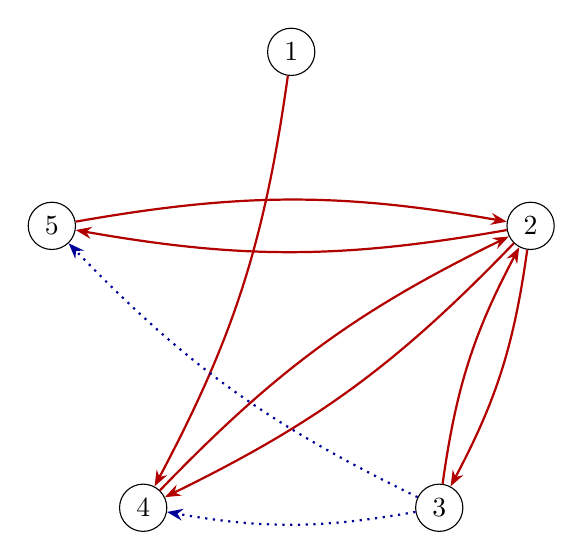
\begin{tikzpicture}[>={Stealth[length=2mm]}]
\node[draw,circle,minimum size=6mm,inner sep=0pt] (n0) at (0.00,3.20) {1};
\node[draw,circle,minimum size=6mm,inner sep=0pt] (n1) at (3.04,0.99) {2};
\node[draw,circle,minimum size=6mm,inner sep=0pt] (n2) at (1.88,-2.59) {3};
\node[draw,circle,minimum size=6mm,inner sep=0pt] (n3) at (-1.88,-2.59) {4};
\node[draw,circle,minimum size=6mm,inner sep=0pt] (n4) at (-3.04,0.99) {5};
\draw[->,red!70!black,thick] (n0) to[bend left=10] (n3);
\draw[->,red!70!black,thick] (n1) to[bend left=10] (n2);
\draw[->,red!70!black,thick] (n1) to[bend left=10] (n3);
\draw[->,red!70!black,thick] (n1) to[bend left=10] (n4);
\draw[->,red!70!black,thick] (n2) to[bend left=10] (n1);
\draw[->,red!70!black,thick] (n3) to[bend left=10] (n1);
\draw[->,red!70!black,thick] (n4) to[bend left=10] (n1);
\draw[->,blue!60!black,thick,dotted] (n2) to[bend left=10] (n3);
\draw[->,blue!60!black,thick,dotted] (n2) to[bend left=10] (n4);
\end{tikzpicture}
\end{center}
\noindent Solid: defeats. Dashed: supports. Dotted: one party's case is part of another's.
\begin{enumerate}
\item Mark 7: God’s word judges human tradition
\item Sola scriptura from Mark 7
\item Trent (Tradition II)
\item Trent (Tradition II), read as commandments of men
\item Trent (Tradition II), read as the apostolic word handed on unwritten
\end{enumerate}
\begin{longtable}{@{}>{\raggedright\arraybackslash}p{0.3\textwidth} >{\raggedright\arraybackslash}p{0.3\textwidth} >{\raggedright\arraybackslash}p{0.3\textwidth}@{}}
\toprule
\textbf{From} & \textbf{To} & \textbf{Edge} \\
\midrule
\endhead
1 \emph{Mark 7: God’s word judges human tradition} & 4 \emph{Trent (Tradition II), read as commandments of men} & defeats \\
2 \emph{Sola scriptura from Mark 7} & 3 \emph{Trent (Tradition II)} & defeats \\
2 \emph{Sola scriptura from Mark 7} & 4 \emph{Trent (Tradition II), read as commandments of men} & defeats \\
2 \emph{Sola scriptura from Mark 7} & 5 \emph{Trent (Tradition II), read as the apostolic word handed on unwritten} & defeats \\
3 \emph{Trent (Tradition II)} & 2 \emph{Sola scriptura from Mark 7} & defeats \\
4 \emph{Trent (Tradition II), read as commandments of men} & 2 \emph{Sola scriptura from Mark 7} & defeats \\
5 \emph{Trent (Tradition II), read as the apostolic word handed on unwritten} & 2 \emph{Sola scriptura from Mark 7} & defeats \\
3 \emph{Trent (Tradition II)} & 4 \emph{Trent (Tradition II), read as commandments of men} & is part of \\
3 \emph{Trent (Tradition II)} & 5 \emph{Trent (Tradition II), read as the apostolic word handed on unwritten} & is part of \\
2 \emph{Sola scriptura from Mark 7} & 4 \emph{Trent (Tradition II), read as commandments of men} & attack on a part — already a defeat \\
2 \emph{Sola scriptura from Mark 7} & 5 \emph{Trent (Tradition II), read as the apostolic word handed on unwritten} & attack on a part — already a defeat \\
\bottomrule
\end{longtable}
\noindent The defeats are the cells of \texttt{mark7\allowbreak{}Dispute\_\allowbreak{}defeats}, the supports the cells of \texttt{mark7\allowbreak{}Dispute\_\allowbreak{}supports} and the parts the cells of \texttt{mark7\allowbreak{}Dispute\_\allowbreak{}part\allowbreak{}Of}, each computed from the parties' premises and checked by the kernel. The attacks derived through support and through parts are reported, not counted: every verdict is computed from the defeats alone. Every derived attack is already a defeat.
\par\medskip\noindent\textbf{\texttt{marks\_\allowbreak{}principle\_\allowbreak{}stands\_\allowbreak{}with\_\allowbreak{}trent}}\par\nobreak\noindent
Mark 7’s principle stands with Trent, as Trent states it and read as the apostolic word: Rome’s world, in which the principle holds and apostolic teaching survives outside Scripture.

{\small\begin{verbatim}
theorem marks_principle_stands_with_trent : mark7Dispute.StandTogether
    [Mark7Party.principle, Mark7Party.trent, Mark7Party.trentAsApostolicWord]
-- axioms: propext, Classical.choice, Quot.sound
\end{verbatim}}
\paragraph*{What the dispute decides}
\leavevmode\par\nobreak
\par\medskip\noindent\textbf{\texttt{marks\allowbreak{}Principle\allowbreak{}Unanswered}}\par\nobreak\noindent
How the dispute is settled as far as it can be, in one stage: nothing defeats Mark 7’s principle, so it comes first; and nothing joins it. Mark 7’s case has Trent, and Trent has Mark 7’s case — a standoff; Trent read as the apostolic word has Mark 7’s case; and Trent read as commandments of men has the principle itself.

\paragraph{What the dispute forces is exactly \emph{Mark 7: God’s word judges human tradition}.}
\begin{itemize}
\item Stage 1: \emph{Mark 7: God’s word judges human tradition}.
\begin{itemize}
\item \emph{Mark 7: God’s word judges human tradition} is defeated by nothing.
\end{itemize}
\item Nothing else is forced:
\begin{itemize}
\item \emph{Trent (Tradition II)} defeats \emph{Sola scriptura from Mark 7}, and nothing forced defeats \emph{Trent (Tradition II)}.
\item \emph{Sola scriptura from Mark 7} defeats \emph{Trent (Tradition II)}, and nothing forced defeats \emph{Sola scriptura from Mark 7}.
\item \emph{Mark 7: God’s word judges human tradition} defeats \emph{Trent (Tradition II), read as commandments of men} (\texttt{where\allowbreak{}The\allowbreak{}Mens\allowbreak{}Commandments\allowbreak{}Reading\allowbreak{}Falls}), and nothing forced defeats \emph{Mark 7: God’s word judges human tradition}.
\item \emph{Sola scriptura from Mark 7} defeats \emph{Trent (Tradition II), read as the apostolic word handed on unwritten} (\texttt{where\allowbreak{}The\allowbreak{}Apostolic\allowbreak{}Word\allowbreak{}Reading\allowbreak{}Falls}), and nothing forced defeats \emph{Sola scriptura from Mark 7}.
\end{itemize}
\end{itemize}
\par\noindent\textbf{What this rests on.} The reasons state 4 defeats and 7 absences of defeat, each a cell of the defeat table, \texttt{mark7\allowbreak{}Dispute\_\allowbreak{}defeats}, computed from the two parties' premises and checked by the kernel. Whether an attack survives turns on the attacker's weakest link and on the rating of what it attacks, so a changed rating can change the verdict. The weakest links:
\begin{itemize}
\item \emph{Mark 7: God’s word judges human tradition}, weakest at \emph{well supported}:
\begin{itemize}
\item an inference step --- \cite[Vatican II (1965), Dei Verbum 10]{tanner-decrees-1990}; \cite[IV.x.23]{calvin-institutes-1960}
\end{itemize}
\item \emph{Sola scriptura from Mark 7}, weakest at \emph{disputed}:
\begin{itemize}
\item No apostolic teaching handed on outside Scripture survives, identifiable as the word of God --- \cite[506]{whitaker-disputation-1849}; \cite[I.6]{westminster-confession-1647}
\item an inference step --- \cite{geiselmann-meaning-of-tradition-1966}; \cite[Vatican I (1870), Pastor Aeternus, ch. 4]{tanner-decrees-1990}; \cite{florovsky-bible-church-tradition-1972}
\end{itemize}
\item \emph{Trent (Tradition II)}, weakest at \emph{disputed}:
\begin{itemize}
\item Tradition is a coordinate source of revelation alongside scripture --- \cite[Trent, Session IV (1546), Decree on Sacred Books and Traditions]{tanner-decrees-1990}; \cite{mathison-shape-sola-scriptura-2001}; \cite{geiselmann-meaning-of-tradition-1966}; \cite{congar-tradition-and-traditions-1966}
\end{itemize}
\item \emph{Trent (Tradition II), read as commandments of men}, weakest at \emph{disputed}:
\begin{itemize}
\item Tradition is a coordinate source of revelation alongside scripture --- \cite[Trent, Session IV (1546), Decree on Sacred Books and Traditions]{tanner-decrees-1990}; \cite{mathison-shape-sola-scriptura-2001}; \cite{geiselmann-meaning-of-tradition-1966}; \cite{congar-tradition-and-traditions-1966}
\item an inference step --- \cite[IV.x.23]{calvin-institutes-1960}
\end{itemize}
\item \emph{Trent (Tradition II), read as the apostolic word handed on unwritten}, weakest at \emph{disputed}:
\begin{itemize}
\item Tradition is a coordinate source of revelation alongside scripture --- \cite[Trent, Session IV (1546), Decree on Sacred Books and Traditions]{tanner-decrees-1990}; \cite{mathison-shape-sola-scriptura-2001}; \cite{geiselmann-meaning-of-tradition-1966}; \cite{congar-tradition-and-traditions-1966}
\end{itemize}
\end{itemize}
\noindent Why \emph{Mark 7: God’s word judges human tradition} defeats \emph{Trent (Tradition II), read as commandments of men}, at the level of the claims: \texttt{where\allowbreak{}The\allowbreak{}Mens\allowbreak{}Commandments\allowbreak{}Reading\allowbreak{}Falls}.
\noindent Why \emph{Sola scriptura from Mark 7} defeats \emph{Trent (Tradition II), read as the apostolic word handed on unwritten}, at the level of the claims: \texttt{where\allowbreak{}The\allowbreak{}Apostolic\allowbreak{}Word\allowbreak{}Reading\allowbreak{}Falls}.
\par\medskip\noindent\textbf{\texttt{marks\_\allowbreak{}principle\_\allowbreak{}prevails}}\par\nobreak\noindent
\textbf{Mark 7’s principle prevails outright, and it is common ground.} The grounded extension — what the dispute forces before any choice between rivals — is exactly the principle: God’s word judges human tradition, and no commandment of men may be taught as God’s word. Nothing defeats it: the one party that contradicts it, Trent read as commandments of men, rests on a reading rated \texttt{disputed}, and its reply fails against a principle whose every link is rated \texttt{well\allowbreak{}Supported} or better. And Trent, as it states its position, does not contradict it at all (\texttt{trent\_\allowbreak{}grants\_\allowbreak{}marks\_\allowbreak{}principle}).

What this does not claim: that sola scriptura is forced. Mark 7’s case for it is not (\texttt{mark7\_\allowbreak{}case\_\allowbreak{}not\_\allowbreak{}forced}).

{\small\begin{verbatim}
theorem marks_principle_prevails : Framework.grounded mark7Dispute.defeats =
    {Mark7Party.principle}
-- axioms: propext, Classical.choice, Quot.sound
\end{verbatim}}
\par\medskip\noindent\textbf{\texttt{mens\allowbreak{}Commandments\allowbreak{}Reading\allowbreak{}Answered}}\par\nobreak\noindent
Why Trent, read as commandments of men, cannot be defended: Mark 7’s principle defeats it, and nothing defeats the principle.

\paragraph{\emph{Trent (Tradition II), read as commandments of men} cannot be defended: no admissible position holds it.}
\begin{itemize}
\item \emph{Mark 7: God’s word judges human tradition} defeats \emph{Trent (Tradition II), read as commandments of men} (\texttt{where\allowbreak{}The\allowbreak{}Mens\allowbreak{}Commandments\allowbreak{}Reading\allowbreak{}Falls}), and nothing defeats \emph{Mark 7: God’s word judges human tradition}.
\end{itemize}
\par\noindent\textbf{What this rests on.} The reasons state 1 defeat and 5 absences of defeat, each a cell of the defeat table, \texttt{mark7\allowbreak{}Dispute\_\allowbreak{}defeats}, computed from the two parties' premises and checked by the kernel. Whether an attack survives turns on the attacker's weakest link and on the rating of what it attacks, so a changed rating can change the verdict. The weakest links:
\begin{itemize}
\item \emph{Mark 7: God’s word judges human tradition}, weakest at \emph{well supported}:
\begin{itemize}
\item an inference step --- \cite[Vatican II (1965), Dei Verbum 10]{tanner-decrees-1990}; \cite[IV.x.23]{calvin-institutes-1960}
\end{itemize}
\item \emph{Trent (Tradition II), read as commandments of men}, weakest at \emph{disputed}:
\begin{itemize}
\item Tradition is a coordinate source of revelation alongside scripture --- \cite[Trent, Session IV (1546), Decree on Sacred Books and Traditions]{tanner-decrees-1990}; \cite{mathison-shape-sola-scriptura-2001}; \cite{geiselmann-meaning-of-tradition-1966}; \cite{congar-tradition-and-traditions-1966}
\item an inference step --- \cite[IV.x.23]{calvin-institutes-1960}
\end{itemize}
\item \emph{Sola scriptura from Mark 7}, weakest at \emph{disputed}:
\begin{itemize}
\item No apostolic teaching handed on outside Scripture survives, identifiable as the word of God --- \cite[506]{whitaker-disputation-1849}; \cite[I.6]{westminster-confession-1647}
\item an inference step --- \cite{geiselmann-meaning-of-tradition-1966}; \cite[Vatican I (1870), Pastor Aeternus, ch. 4]{tanner-decrees-1990}; \cite{florovsky-bible-church-tradition-1972}
\end{itemize}
\item \emph{Trent (Tradition II)}, weakest at \emph{disputed}:
\begin{itemize}
\item Tradition is a coordinate source of revelation alongside scripture --- \cite[Trent, Session IV (1546), Decree on Sacred Books and Traditions]{tanner-decrees-1990}; \cite{mathison-shape-sola-scriptura-2001}; \cite{geiselmann-meaning-of-tradition-1966}; \cite{congar-tradition-and-traditions-1966}
\end{itemize}
\item \emph{Trent (Tradition II), read as the apostolic word handed on unwritten}, weakest at \emph{disputed}:
\begin{itemize}
\item Tradition is a coordinate source of revelation alongside scripture --- \cite[Trent, Session IV (1546), Decree on Sacred Books and Traditions]{tanner-decrees-1990}; \cite{mathison-shape-sola-scriptura-2001}; \cite{geiselmann-meaning-of-tradition-1966}; \cite{congar-tradition-and-traditions-1966}
\end{itemize}
\end{itemize}
\noindent Why \emph{Mark 7: God’s word judges human tradition} defeats \emph{Trent (Tradition II), read as commandments of men}, at the level of the claims: \texttt{where\allowbreak{}The\allowbreak{}Mens\allowbreak{}Commandments\allowbreak{}Reading\allowbreak{}Falls}.
\par\medskip\noindent\textbf{\texttt{trent\_\allowbreak{}as\_\allowbreak{}mens\_\allowbreak{}commandments\_\allowbreak{}indefensible}}\par\nobreak\noindent
\textbf{Trent, read as commandments of men, cannot be defended.} No consistent position that answers its attackers can hold it: Mark 7’s principle defeats it, and nothing answers the principle. This is the first horn of \texttt{what\allowbreak{}Trents\allowbreak{}Tradition\allowbreak{}Is}, weighed: if what Trent receives alongside Scripture were a commandment of men, Jesus’ words in Mark 7 would condemn it, at a step rated \texttt{well\allowbreak{}Supported}.

What this does not claim: that Trent’s tradition \emph{is} a commandment of men. Trent says the opposite, and Calvin’s reading of it is rated \texttt{disputed}.

{\small\begin{verbatim}
theorem trent_as_mens_commandments_indefensible : ∀ (S : Set Mark7Party),
    Framework.Admissible mark7Dispute.defeats S →
    Mark7Party.trentAsMensCommandments ∉ S
-- axioms: propext, Classical.choice, Quot.sound
\end{verbatim}}
\par\medskip\noindent\textbf{\texttt{mark7\allowbreak{}Stands\allowbreak{}With\allowbreak{}Its\allowbreak{}Principle}}\par\nobreak\noindent
Why Mark 7’s case can be defended: it stands with Mark 7’s principle, and answers every party that defeats it — Trent, read or unread — itself.

\paragraph{\emph{Sola scriptura from Mark 7} is accepted on some resolution.}
\begin{itemize}
\item A position holding \emph{Mark 7: God’s word judges human tradition}, \emph{Sola scriptura from Mark 7} can be held.
\item None of \emph{Mark 7: God’s word judges human tradition}, \emph{Sola scriptura from Mark 7} defeats another, and each attack on them is answered from among them:
\begin{itemize}
\item \emph{Trent (Tradition II)} defeats \emph{Sola scriptura from Mark 7}, and \emph{Sola scriptura from Mark 7} defeats \emph{Trent (Tradition II)}.
\item \emph{Trent (Tradition II), read as commandments of men} defeats \emph{Sola scriptura from Mark 7}, and \emph{Mark 7: God’s word judges human tradition} defeats \emph{Trent (Tradition II), read as commandments of men} (\texttt{where\allowbreak{}The\allowbreak{}Mens\allowbreak{}Commandments\allowbreak{}Reading\allowbreak{}Falls}).
\item \emph{Trent (Tradition II), read as the apostolic word handed on unwritten} defeats \emph{Sola scriptura from Mark 7}, and \emph{Sola scriptura from Mark 7} defeats \emph{Trent (Tradition II), read as the apostolic word handed on unwritten} (\texttt{where\allowbreak{}The\allowbreak{}Apostolic\allowbreak{}Word\allowbreak{}Reading\allowbreak{}Falls}).
\end{itemize}
\end{itemize}
\par\noindent\textbf{What this rests on.} The reasons state 6 defeats and 7 absences of defeat, each a cell of the defeat table, \texttt{mark7\allowbreak{}Dispute\_\allowbreak{}defeats}, computed from the two parties' premises and checked by the kernel. Whether an attack survives turns on the attacker's weakest link and on the rating of what it attacks, so a changed rating can change the verdict. The weakest links:
\begin{itemize}
\item \emph{Mark 7: God’s word judges human tradition}, weakest at \emph{well supported}:
\begin{itemize}
\item an inference step --- \cite[Vatican II (1965), Dei Verbum 10]{tanner-decrees-1990}; \cite[IV.x.23]{calvin-institutes-1960}
\end{itemize}
\item \emph{Sola scriptura from Mark 7}, weakest at \emph{disputed}:
\begin{itemize}
\item No apostolic teaching handed on outside Scripture survives, identifiable as the word of God --- \cite[506]{whitaker-disputation-1849}; \cite[I.6]{westminster-confession-1647}
\item an inference step --- \cite{geiselmann-meaning-of-tradition-1966}; \cite[Vatican I (1870), Pastor Aeternus, ch. 4]{tanner-decrees-1990}; \cite{florovsky-bible-church-tradition-1972}
\end{itemize}
\item \emph{Trent (Tradition II)}, weakest at \emph{disputed}:
\begin{itemize}
\item Tradition is a coordinate source of revelation alongside scripture --- \cite[Trent, Session IV (1546), Decree on Sacred Books and Traditions]{tanner-decrees-1990}; \cite{mathison-shape-sola-scriptura-2001}; \cite{geiselmann-meaning-of-tradition-1966}; \cite{congar-tradition-and-traditions-1966}
\end{itemize}
\item \emph{Trent (Tradition II), read as commandments of men}, weakest at \emph{disputed}:
\begin{itemize}
\item Tradition is a coordinate source of revelation alongside scripture --- \cite[Trent, Session IV (1546), Decree on Sacred Books and Traditions]{tanner-decrees-1990}; \cite{mathison-shape-sola-scriptura-2001}; \cite{geiselmann-meaning-of-tradition-1966}; \cite{congar-tradition-and-traditions-1966}
\item an inference step --- \cite[IV.x.23]{calvin-institutes-1960}
\end{itemize}
\item \emph{Trent (Tradition II), read as the apostolic word handed on unwritten}, weakest at \emph{disputed}:
\begin{itemize}
\item Tradition is a coordinate source of revelation alongside scripture --- \cite[Trent, Session IV (1546), Decree on Sacred Books and Traditions]{tanner-decrees-1990}; \cite{mathison-shape-sola-scriptura-2001}; \cite{geiselmann-meaning-of-tradition-1966}; \cite{congar-tradition-and-traditions-1966}
\end{itemize}
\end{itemize}
\noindent Why \emph{Mark 7: God’s word judges human tradition} defeats \emph{Trent (Tradition II), read as commandments of men}, at the level of the claims: \texttt{where\allowbreak{}The\allowbreak{}Mens\allowbreak{}Commandments\allowbreak{}Reading\allowbreak{}Falls}.
\noindent Why \emph{Sola scriptura from Mark 7} defeats \emph{Trent (Tradition II), read as the apostolic word handed on unwritten}, at the level of the claims: \texttt{where\allowbreak{}The\allowbreak{}Apostolic\allowbreak{}Word\allowbreak{}Reading\allowbreak{}Falls}.
\par\medskip\noindent\textbf{\texttt{mark7\_\allowbreak{}case\_\allowbreak{}defensible}}\par\nobreak\noindent
\textbf{Sola scriptura from Mark 7 can be defended.} Some maximal defensible position holds it, with Mark 7’s principle. Every party that defeats it — Trent, as it states its position and read either way — it defeats back.

{\small\begin{verbatim}
theorem mark7_case_defensible : Framework.CredulouslyAccepted
    mark7Dispute.defeats Mark7Party.mark7
-- axioms: propext, Classical.choice, Quot.sound
\end{verbatim}}
\par\medskip\noindent\textbf{\texttt{mark7\allowbreak{}Answered\allowbreak{}By\allowbreak{}Trent}}\par\nobreak\noindent
Why Mark 7’s case is not forced: a defensible position holds Trent, and Trent defeats it.

\paragraph{\emph{Sola scriptura from Mark 7} is not accepted on every resolution.}
\begin{itemize}
\item A position holding \emph{Mark 7: God’s word judges human tradition}, \emph{Trent (Tradition II)}, \emph{Trent (Tradition II), read as the apostolic word handed on unwritten} can be held, and it holds \emph{Trent (Tradition II)}; \emph{Trent (Tradition II)} conflicts with \emph{Sola scriptura from Mark 7}: \emph{Trent (Tradition II)} defeats \emph{Sola scriptura from Mark 7}, and \emph{Sola scriptura from Mark 7} defeats \emph{Trent (Tradition II)}.
\item None of \emph{Mark 7: God’s word judges human tradition}, \emph{Trent (Tradition II)}, \emph{Trent (Tradition II), read as the apostolic word handed on unwritten} defeats another, and each attack on them is answered from among them:
\begin{itemize}
\item \emph{Sola scriptura from Mark 7} defeats \emph{Trent (Tradition II)}, and \emph{Trent (Tradition II)} defeats \emph{Sola scriptura from Mark 7}.
\item \emph{Sola scriptura from Mark 7} defeats \emph{Trent (Tradition II), read as the apostolic word handed on unwritten} (\texttt{where\allowbreak{}The\allowbreak{}Apostolic\allowbreak{}Word\allowbreak{}Reading\allowbreak{}Falls}), and \emph{Trent (Tradition II)} defeats \emph{Sola scriptura from Mark 7}.
\end{itemize}
\end{itemize}
\par\noindent\textbf{What this rests on.} The reasons state 3 defeats and 13 absences of defeat, each a cell of the defeat table, \texttt{mark7\allowbreak{}Dispute\_\allowbreak{}defeats}, computed from the two parties' premises and checked by the kernel. Whether an attack survives turns on the attacker's weakest link and on the rating of what it attacks, so a changed rating can change the verdict. The weakest links:
\begin{itemize}
\item \emph{Trent (Tradition II)}, weakest at \emph{disputed}:
\begin{itemize}
\item Tradition is a coordinate source of revelation alongside scripture --- \cite[Trent, Session IV (1546), Decree on Sacred Books and Traditions]{tanner-decrees-1990}; \cite{mathison-shape-sola-scriptura-2001}; \cite{geiselmann-meaning-of-tradition-1966}; \cite{congar-tradition-and-traditions-1966}
\end{itemize}
\item \emph{Sola scriptura from Mark 7}, weakest at \emph{disputed}:
\begin{itemize}
\item No apostolic teaching handed on outside Scripture survives, identifiable as the word of God --- \cite[506]{whitaker-disputation-1849}; \cite[I.6]{westminster-confession-1647}
\item an inference step --- \cite{geiselmann-meaning-of-tradition-1966}; \cite[Vatican I (1870), Pastor Aeternus, ch. 4]{tanner-decrees-1990}; \cite{florovsky-bible-church-tradition-1972}
\end{itemize}
\item \emph{Mark 7: God’s word judges human tradition}, weakest at \emph{well supported}:
\begin{itemize}
\item an inference step --- \cite[Vatican II (1965), Dei Verbum 10]{tanner-decrees-1990}; \cite[IV.x.23]{calvin-institutes-1960}
\end{itemize}
\item \emph{Trent (Tradition II), read as the apostolic word handed on unwritten}, weakest at \emph{disputed}:
\begin{itemize}
\item Tradition is a coordinate source of revelation alongside scripture --- \cite[Trent, Session IV (1546), Decree on Sacred Books and Traditions]{tanner-decrees-1990}; \cite{mathison-shape-sola-scriptura-2001}; \cite{geiselmann-meaning-of-tradition-1966}; \cite{congar-tradition-and-traditions-1966}
\end{itemize}
\item \emph{Trent (Tradition II), read as commandments of men}, weakest at \emph{disputed}:
\begin{itemize}
\item Tradition is a coordinate source of revelation alongside scripture --- \cite[Trent, Session IV (1546), Decree on Sacred Books and Traditions]{tanner-decrees-1990}; \cite{mathison-shape-sola-scriptura-2001}; \cite{geiselmann-meaning-of-tradition-1966}; \cite{congar-tradition-and-traditions-1966}
\item an inference step --- \cite[IV.x.23]{calvin-institutes-1960}
\end{itemize}
\end{itemize}
\noindent Why \emph{Sola scriptura from Mark 7} defeats \emph{Trent (Tradition II), read as the apostolic word handed on unwritten}, at the level of the claims: \texttt{where\allowbreak{}The\allowbreak{}Apostolic\allowbreak{}Word\allowbreak{}Reading\allowbreak{}Falls}.
\par\medskip\noindent\textbf{\texttt{mark7\_\allowbreak{}case\_\allowbreak{}not\_\allowbreak{}forced}}\par\nobreak\noindent
\textbf{Nor is it forced.} A maximal defensible position holds Trent, with Mark 7’s principle and with Trent read as the apostolic word, and cannot hold Mark 7’s case with it. Their weakest links are all \texttt{disputed}, so no rating breaks the tie. What would decide it is argued, not weighed: whether any apostolic word survives outside Scripture (\texttt{where\allowbreak{}The\allowbreak{}Apostolic\allowbreak{}Word\allowbreak{}Reading\allowbreak{}Falls}), and, even granting that none does, whether the principle then makes Scripture the \emph{sole} infallible rule — a step Geiselmann and Florovsky deny.

{\small\begin{verbatim}
theorem mark7_case_not_forced : ¬Framework.SkepticallyAccepted
    mark7Dispute.defeats Mark7Party.mark7
-- axioms: propext, Classical.choice, Quot.sound
\end{verbatim}}
\par\medskip\noindent\textbf{\texttt{trent\allowbreak{}Stands\allowbreak{}With\allowbreak{}Marks\allowbreak{}Principle}}\par\nobreak\noindent
Why Trent can be defended against Mark 7: it stands with Mark 7’s principle and with its own reading as the apostolic word, and answers Mark 7’s case itself.

\paragraph{\emph{Trent (Tradition II)} is accepted on some resolution.}
\begin{itemize}
\item A position holding \emph{Mark 7: God’s word judges human tradition}, \emph{Trent (Tradition II)}, \emph{Trent (Tradition II), read as the apostolic word handed on unwritten} can be held.
\item None of \emph{Mark 7: God’s word judges human tradition}, \emph{Trent (Tradition II)}, \emph{Trent (Tradition II), read as the apostolic word handed on unwritten} defeats another, and each attack on them is answered from among them:
\begin{itemize}
\item \emph{Sola scriptura from Mark 7} defeats \emph{Trent (Tradition II)}, and \emph{Trent (Tradition II)} defeats \emph{Sola scriptura from Mark 7}.
\item \emph{Sola scriptura from Mark 7} defeats \emph{Trent (Tradition II), read as the apostolic word handed on unwritten} (\texttt{where\allowbreak{}The\allowbreak{}Apostolic\allowbreak{}Word\allowbreak{}Reading\allowbreak{}Falls}), and \emph{Trent (Tradition II)} defeats \emph{Sola scriptura from Mark 7}.
\end{itemize}
\end{itemize}
\par\noindent\textbf{What this rests on.} The reasons state 3 defeats and 13 absences of defeat, each a cell of the defeat table, \texttt{mark7\allowbreak{}Dispute\_\allowbreak{}defeats}, computed from the two parties' premises and checked by the kernel. Whether an attack survives turns on the attacker's weakest link and on the rating of what it attacks, so a changed rating can change the verdict. The weakest links:
\begin{itemize}
\item \emph{Mark 7: God’s word judges human tradition}, weakest at \emph{well supported}:
\begin{itemize}
\item an inference step --- \cite[Vatican II (1965), Dei Verbum 10]{tanner-decrees-1990}; \cite[IV.x.23]{calvin-institutes-1960}
\end{itemize}
\item \emph{Trent (Tradition II)}, weakest at \emph{disputed}:
\begin{itemize}
\item Tradition is a coordinate source of revelation alongside scripture --- \cite[Trent, Session IV (1546), Decree on Sacred Books and Traditions]{tanner-decrees-1990}; \cite{mathison-shape-sola-scriptura-2001}; \cite{geiselmann-meaning-of-tradition-1966}; \cite{congar-tradition-and-traditions-1966}
\end{itemize}
\item \emph{Trent (Tradition II), read as the apostolic word handed on unwritten}, weakest at \emph{disputed}:
\begin{itemize}
\item Tradition is a coordinate source of revelation alongside scripture --- \cite[Trent, Session IV (1546), Decree on Sacred Books and Traditions]{tanner-decrees-1990}; \cite{mathison-shape-sola-scriptura-2001}; \cite{geiselmann-meaning-of-tradition-1966}; \cite{congar-tradition-and-traditions-1966}
\end{itemize}
\item \emph{Sola scriptura from Mark 7}, weakest at \emph{disputed}:
\begin{itemize}
\item No apostolic teaching handed on outside Scripture survives, identifiable as the word of God --- \cite[506]{whitaker-disputation-1849}; \cite[I.6]{westminster-confession-1647}
\item an inference step --- \cite{geiselmann-meaning-of-tradition-1966}; \cite[Vatican I (1870), Pastor Aeternus, ch. 4]{tanner-decrees-1990}; \cite{florovsky-bible-church-tradition-1972}
\end{itemize}
\item \emph{Trent (Tradition II), read as commandments of men}, weakest at \emph{disputed}:
\begin{itemize}
\item Tradition is a coordinate source of revelation alongside scripture --- \cite[Trent, Session IV (1546), Decree on Sacred Books and Traditions]{tanner-decrees-1990}; \cite{mathison-shape-sola-scriptura-2001}; \cite{geiselmann-meaning-of-tradition-1966}; \cite{congar-tradition-and-traditions-1966}
\item an inference step --- \cite[IV.x.23]{calvin-institutes-1960}
\end{itemize}
\end{itemize}
\noindent Why \emph{Sola scriptura from Mark 7} defeats \emph{Trent (Tradition II), read as the apostolic word handed on unwritten}, at the level of the claims: \texttt{where\allowbreak{}The\allowbreak{}Apostolic\allowbreak{}Word\allowbreak{}Reading\allowbreak{}Falls}.
\par\medskip\noindent\textbf{\texttt{trent\_\allowbreak{}defensible\_\allowbreak{}against\_\allowbreak{}mark7}}\par\nobreak\noindent
\textbf{Trent, as it states its position, can be defended against Mark 7} — and with Mark 7’s principle. Some maximal defensible position holds Trent, the principle, and Trent read as the apostolic word. Granting everything Mark 7’s principle says costs Trent nothing, so long as what it receives is the apostolic word and not a commandment of men.

{\small\begin{verbatim}
theorem trent_defensible_against_mark7 : Framework.CredulouslyAccepted
    mark7Dispute.defeats Mark7Party.trent
-- axioms: propext, Classical.choice, Quot.sound
\end{verbatim}}
\par\medskip\noindent\textbf{\texttt{trent\allowbreak{}Answered\allowbreak{}By\allowbreak{}Mark7}}\par\nobreak\noindent
Why Trent is not forced: a defensible position holds Mark 7’s case, and it defeats Trent.

\paragraph{\emph{Trent (Tradition II)} is not accepted on every resolution.}
\begin{itemize}
\item A position holding \emph{Mark 7: God’s word judges human tradition}, \emph{Sola scriptura from Mark 7} can be held, and it holds \emph{Sola scriptura from Mark 7}; \emph{Sola scriptura from Mark 7} conflicts with \emph{Trent (Tradition II)}: \emph{Sola scriptura from Mark 7} defeats \emph{Trent (Tradition II)}, and \emph{Trent (Tradition II)} defeats \emph{Sola scriptura from Mark 7}.
\item None of \emph{Mark 7: God’s word judges human tradition}, \emph{Sola scriptura from Mark 7} defeats another, and each attack on them is answered from among them:
\begin{itemize}
\item \emph{Trent (Tradition II)} defeats \emph{Sola scriptura from Mark 7}, and \emph{Sola scriptura from Mark 7} defeats \emph{Trent (Tradition II)}.
\item \emph{Trent (Tradition II), read as commandments of men} defeats \emph{Sola scriptura from Mark 7}, and \emph{Mark 7: God’s word judges human tradition} defeats \emph{Trent (Tradition II), read as commandments of men} (\texttt{where\allowbreak{}The\allowbreak{}Mens\allowbreak{}Commandments\allowbreak{}Reading\allowbreak{}Falls}).
\item \emph{Trent (Tradition II), read as the apostolic word handed on unwritten} defeats \emph{Sola scriptura from Mark 7}, and \emph{Sola scriptura from Mark 7} defeats \emph{Trent (Tradition II), read as the apostolic word handed on unwritten} (\texttt{where\allowbreak{}The\allowbreak{}Apostolic\allowbreak{}Word\allowbreak{}Reading\allowbreak{}Falls}).
\end{itemize}
\end{itemize}
\par\noindent\textbf{What this rests on.} The reasons state 6 defeats and 7 absences of defeat, each a cell of the defeat table, \texttt{mark7\allowbreak{}Dispute\_\allowbreak{}defeats}, computed from the two parties' premises and checked by the kernel. Whether an attack survives turns on the attacker's weakest link and on the rating of what it attacks, so a changed rating can change the verdict. The weakest links:
\begin{itemize}
\item \emph{Sola scriptura from Mark 7}, weakest at \emph{disputed}:
\begin{itemize}
\item No apostolic teaching handed on outside Scripture survives, identifiable as the word of God --- \cite[506]{whitaker-disputation-1849}; \cite[I.6]{westminster-confession-1647}
\item an inference step --- \cite{geiselmann-meaning-of-tradition-1966}; \cite[Vatican I (1870), Pastor Aeternus, ch. 4]{tanner-decrees-1990}; \cite{florovsky-bible-church-tradition-1972}
\end{itemize}
\item \emph{Trent (Tradition II)}, weakest at \emph{disputed}:
\begin{itemize}
\item Tradition is a coordinate source of revelation alongside scripture --- \cite[Trent, Session IV (1546), Decree on Sacred Books and Traditions]{tanner-decrees-1990}; \cite{mathison-shape-sola-scriptura-2001}; \cite{geiselmann-meaning-of-tradition-1966}; \cite{congar-tradition-and-traditions-1966}
\end{itemize}
\item \emph{Mark 7: God’s word judges human tradition}, weakest at \emph{well supported}:
\begin{itemize}
\item an inference step --- \cite[Vatican II (1965), Dei Verbum 10]{tanner-decrees-1990}; \cite[IV.x.23]{calvin-institutes-1960}
\end{itemize}
\item \emph{Trent (Tradition II), read as commandments of men}, weakest at \emph{disputed}:
\begin{itemize}
\item Tradition is a coordinate source of revelation alongside scripture --- \cite[Trent, Session IV (1546), Decree on Sacred Books and Traditions]{tanner-decrees-1990}; \cite{mathison-shape-sola-scriptura-2001}; \cite{geiselmann-meaning-of-tradition-1966}; \cite{congar-tradition-and-traditions-1966}
\item an inference step --- \cite[IV.x.23]{calvin-institutes-1960}
\end{itemize}
\item \emph{Trent (Tradition II), read as the apostolic word handed on unwritten}, weakest at \emph{disputed}:
\begin{itemize}
\item Tradition is a coordinate source of revelation alongside scripture --- \cite[Trent, Session IV (1546), Decree on Sacred Books and Traditions]{tanner-decrees-1990}; \cite{mathison-shape-sola-scriptura-2001}; \cite{geiselmann-meaning-of-tradition-1966}; \cite{congar-tradition-and-traditions-1966}
\end{itemize}
\end{itemize}
\noindent Why \emph{Mark 7: God’s word judges human tradition} defeats \emph{Trent (Tradition II), read as commandments of men}, at the level of the claims: \texttt{where\allowbreak{}The\allowbreak{}Mens\allowbreak{}Commandments\allowbreak{}Reading\allowbreak{}Falls}.
\noindent Why \emph{Sola scriptura from Mark 7} defeats \emph{Trent (Tradition II), read as the apostolic word handed on unwritten}, at the level of the claims: \texttt{where\allowbreak{}The\allowbreak{}Apostolic\allowbreak{}Word\allowbreak{}Reading\allowbreak{}Falls}.
\par\medskip\noindent\textbf{\texttt{trent\_\allowbreak{}not\_\allowbreak{}forced\_\allowbreak{}against\_\allowbreak{}mark7}}\par\nobreak\noindent
\textbf{Nor is Trent forced.} A maximal defensible position holds Mark 7’s case for sola scriptura, and cannot hold Trent with it. Between them the dispute chooses neither.

{\small\begin{verbatim}
theorem trent_not_forced_against_mark7 : ¬Framework.SkepticallyAccepted
    mark7Dispute.defeats Mark7Party.trent
-- axioms: propext, Classical.choice, Quot.sound
\end{verbatim}}
\subsection*{TestimonyArguments.SolaScriptura.Hearings — Mark 7, heard against each reading of Trent}
The dispute over Mark 7 hears Trent three ways at once: as Trent states its position, and with its tradition read each of the two ways the dilemma \texttt{what\allowbreak{}Trents\allowbreak{}Tradition\allowbreak{}Is} names. A reader usually has one reading in mind, and asks what Mark 7 settles \emph{if that is what Trent means}. Each question is answered by hearing the same dispute with the other readings set aside. Nothing is re-argued: a hearing keeps every defeat the full dispute proved.

\textbf{If Rome’s tradition were the commandments of men, would Mark 7 settle sola scriptura?} Heard against that reading alone (\texttt{mens\allowbreak{}Commandments\allowbreak{}Hearing}), Mark 7’s case is forced — but only because nothing left in the hearing contests it. The reading is the only party that attacks it, and the principle defeats the reading. Mark 7’s case still rests on two things rated \texttt{disputed}: that no apostolic word survives outside Scripture, and the step from the principle to the \emph{sole} rule. The reading of Trent as commandments of men contests neither, and the parties that would are set aside. This is the Protestant polemic at full strength — and it holds only on a reading of Trent that Trent itself denies.

\textbf{If Rome’s tradition is the apostolic word handed on unwritten, what does Mark 7 settle?} Heard against that reading (\texttt{apostolic\allowbreak{}Word\allowbreak{}Hearing}), only the principle — which the reading grants. Mark 7’s case and the reading defeat each other at one premise, that no apostolic word survives outside Scripture, and each side’s weakest link is \texttt{disputed}. So the dispute chooses neither.

The difference between the two hearings is the whole of what Mark 7 contributes: against Rome’s tradition read as human, it leaves Mark 7’s case unopposed; against it read as apostolic, it leaves the question where it was. Which it is, Mark 7 does not say.

\paragraph*{Heard against the reading as commandments of men}
\leavevmode\par\nobreak
\par\medskip\noindent\textbf{\texttt{mens\allowbreak{}Commandments\allowbreak{}Hearing}}\par\nobreak\noindent
Mark 7’s principle and case, heard against Trent read as commandments of men. Not heard: Trent as it states its position, and Trent read as the apostolic word.

{\small\begin{verbatim}
def mensCommandmentsHearing : Dispute Claim { i // i ∈ [Mark7Party.principle,
    Mark7Party.mark7, Mark7Party.trentAsMensCommandments] } :=
  mark7Dispute.restrict fun x =>
    x ∈
      [Mark7Party.principle, Mark7Party.mark7,
        Mark7Party.trentAsMensCommandments]
\end{verbatim}}
\par\medskip\noindent\textbf{\texttt{mens\allowbreak{}Commandments\allowbreak{}Hearing\allowbreak{}Settles}}\par\nobreak\noindent
How the hearing is settled, in two stages: nothing defeats Mark 7’s principle, so it comes first; the principle defeats the reading, and with the reading answered Mark 7’s case has no attacker left, so it comes second.

\paragraph{What the dispute forces is exactly \emph{Mark 7: God’s word judges human tradition}, \emph{Sola scriptura from Mark 7}.}
\begin{itemize}
\item Stage 1: \emph{Mark 7: God’s word judges human tradition}.
\begin{itemize}
\item \emph{Mark 7: God’s word judges human tradition} is defeated by nothing.
\end{itemize}
\item Stage 2: \emph{Sola scriptura from Mark 7}.
\begin{itemize}
\item \emph{Trent (Tradition II), read as commandments of men} defeats \emph{Sola scriptura from Mark 7}, and \emph{Mark 7: God’s word judges human tradition} defeats \emph{Trent (Tradition II), read as commandments of men} (\texttt{where\allowbreak{}The\allowbreak{}Mens\allowbreak{}Commandments\allowbreak{}Reading\allowbreak{}Falls}).
\end{itemize}
\item Nothing else is forced:
\begin{itemize}
\item \emph{Mark 7: God’s word judges human tradition} defeats \emph{Trent (Tradition II), read as commandments of men} (\texttt{where\allowbreak{}The\allowbreak{}Mens\allowbreak{}Commandments\allowbreak{}Reading\allowbreak{}Falls}), and nothing forced defeats \emph{Mark 7: God’s word judges human tradition}.
\end{itemize}
\end{itemize}
\par\noindent\textbf{What this rests on.} The reasons state 2 defeats and 5 absences of defeat, each a cell of the defeat table, \texttt{mark7\allowbreak{}Dispute\_\allowbreak{}defeats}, computed from the two parties' premises and checked by the kernel. Whether an attack survives turns on the attacker's weakest link and on the rating of what it attacks, so a changed rating can change the verdict. The weakest links:
\begin{itemize}
\item \emph{Mark 7: God’s word judges human tradition}, weakest at \emph{well supported}:
\begin{itemize}
\item an inference step --- \cite[Vatican II (1965), Dei Verbum 10]{tanner-decrees-1990}; \cite[IV.x.23]{calvin-institutes-1960}
\end{itemize}
\item \emph{Sola scriptura from Mark 7}, weakest at \emph{disputed}:
\begin{itemize}
\item No apostolic teaching handed on outside Scripture survives, identifiable as the word of God --- \cite[506]{whitaker-disputation-1849}; \cite[I.6]{westminster-confession-1647}
\item an inference step --- \cite{geiselmann-meaning-of-tradition-1966}; \cite[Vatican I (1870), Pastor Aeternus, ch. 4]{tanner-decrees-1990}; \cite{florovsky-bible-church-tradition-1972}
\end{itemize}
\item \emph{Trent (Tradition II), read as commandments of men}, weakest at \emph{disputed}:
\begin{itemize}
\item Tradition is a coordinate source of revelation alongside scripture --- \cite[Trent, Session IV (1546), Decree on Sacred Books and Traditions]{tanner-decrees-1990}; \cite{mathison-shape-sola-scriptura-2001}; \cite{geiselmann-meaning-of-tradition-1966}; \cite{congar-tradition-and-traditions-1966}
\item an inference step --- \cite[IV.x.23]{calvin-institutes-1960}
\end{itemize}
\end{itemize}
\noindent Why \emph{Mark 7: God’s word judges human tradition} defeats \emph{Trent (Tradition II), read as commandments of men}, at the level of the claims: \texttt{where\allowbreak{}The\allowbreak{}Mens\allowbreak{}Commandments\allowbreak{}Reading\allowbreak{}Falls}.
\par\medskip\noindent\textbf{\texttt{mark7\_\allowbreak{}forced\_\allowbreak{}against\_\allowbreak{}mens\_\allowbreak{}commandments}}\par\nobreak\noindent
\textbf{Against Rome’s tradition read as commandments of men, Mark 7’s case is unopposed.} Heard against that reading alone, Mark 7’s principle and Mark 7’s case for sola scriptura are both forced: the reading is the only party in the hearing that attacks the case, and the principle defeats it.

What this does not claim: that Rome’s tradition is the commandments of men — Trent says what it receives came from Christ and the apostles, and the reading that says otherwise is rated \texttt{disputed}. Nor that Mark 7’s case is sound. It still rests on the premise that no apostolic word survives outside Scripture, and on a step Geiselmann and Florovsky deny, both \texttt{disputed}; no party heard here contests either. Trent as it states its position, and Trent read as the apostolic word, are set aside.

{\small\begin{verbatim}
theorem mark7_forced_against_mens_commandments : Framework.grounded
    mensCommandmentsHearing.defeats = Solver.toSet (Witness.listSub
    (Membership.mem [Mark7Party.principle, Mark7Party.mark7,
    Mark7Party.trentAsMensCommandments]) [Mark7Party.principle,
    Mark7Party.mark7])
-- axioms: propext, Classical.choice, Quot.sound
\end{verbatim}}
\paragraph*{Heard against the reading as the apostolic word}
\leavevmode\par\nobreak
\par\medskip\noindent\textbf{\texttt{apostolic\allowbreak{}Word\allowbreak{}Hearing}}\par\nobreak\noindent
Mark 7’s principle and case, heard against Trent read as the apostolic word handed on unwritten. Not heard: Trent as it states its position, and Trent read as commandments of men.

{\small\begin{verbatim}
def apostolicWordHearing : Dispute Claim { i // i ∈ [Mark7Party.principle,
    Mark7Party.mark7, Mark7Party.trentAsApostolicWord] } :=
  mark7Dispute.restrict fun x =>
    x ∈
      [Mark7Party.principle, Mark7Party.mark7,
        Mark7Party.trentAsApostolicWord]
\end{verbatim}}
\par\medskip\noindent\textbf{\texttt{apostolic\allowbreak{}Word\allowbreak{}Hearing\allowbreak{}Settles}}\par\nobreak\noindent
How the hearing is settled: nothing defeats Mark 7’s principle, so it comes first; and nothing joins it, because Mark 7’s case and the reading defeat each other.

\paragraph{What the dispute forces is exactly \emph{Mark 7: God’s word judges human tradition}.}
\begin{itemize}
\item Stage 1: \emph{Mark 7: God’s word judges human tradition}.
\begin{itemize}
\item \emph{Mark 7: God’s word judges human tradition} is defeated by nothing.
\end{itemize}
\item Nothing else is forced:
\begin{itemize}
\item \emph{Trent (Tradition II), read as the apostolic word handed on unwritten} defeats \emph{Sola scriptura from Mark 7}, and nothing forced defeats \emph{Trent (Tradition II), read as the apostolic word handed on unwritten}.
\item \emph{Sola scriptura from Mark 7} defeats \emph{Trent (Tradition II), read as the apostolic word handed on unwritten} (\texttt{where\allowbreak{}The\allowbreak{}Apostolic\allowbreak{}Word\allowbreak{}Reading\allowbreak{}Falls}), and nothing forced defeats \emph{Sola scriptura from Mark 7}.
\end{itemize}
\end{itemize}
\par\noindent\textbf{What this rests on.} The reasons state 2 defeats and 5 absences of defeat, each a cell of the defeat table, \texttt{mark7\allowbreak{}Dispute\_\allowbreak{}defeats}, computed from the two parties' premises and checked by the kernel. Whether an attack survives turns on the attacker's weakest link and on the rating of what it attacks, so a changed rating can change the verdict. The weakest links:
\begin{itemize}
\item \emph{Mark 7: God’s word judges human tradition}, weakest at \emph{well supported}:
\begin{itemize}
\item an inference step --- \cite[Vatican II (1965), Dei Verbum 10]{tanner-decrees-1990}; \cite[IV.x.23]{calvin-institutes-1960}
\end{itemize}
\item \emph{Sola scriptura from Mark 7}, weakest at \emph{disputed}:
\begin{itemize}
\item No apostolic teaching handed on outside Scripture survives, identifiable as the word of God --- \cite[506]{whitaker-disputation-1849}; \cite[I.6]{westminster-confession-1647}
\item an inference step --- \cite{geiselmann-meaning-of-tradition-1966}; \cite[Vatican I (1870), Pastor Aeternus, ch. 4]{tanner-decrees-1990}; \cite{florovsky-bible-church-tradition-1972}
\end{itemize}
\item \emph{Trent (Tradition II), read as the apostolic word handed on unwritten}, weakest at \emph{disputed}:
\begin{itemize}
\item Tradition is a coordinate source of revelation alongside scripture --- \cite[Trent, Session IV (1546), Decree on Sacred Books and Traditions]{tanner-decrees-1990}; \cite{mathison-shape-sola-scriptura-2001}; \cite{geiselmann-meaning-of-tradition-1966}; \cite{congar-tradition-and-traditions-1966}
\end{itemize}
\end{itemize}
\noindent Why \emph{Sola scriptura from Mark 7} defeats \emph{Trent (Tradition II), read as the apostolic word handed on unwritten}, at the level of the claims: \texttt{where\allowbreak{}The\allowbreak{}Apostolic\allowbreak{}Word\allowbreak{}Reading\allowbreak{}Falls}.
\par\medskip\noindent\textbf{\texttt{against\_\allowbreak{}the\_\allowbreak{}apostolic\_\allowbreak{}word\_\allowbreak{}only\_\allowbreak{}the\_\allowbreak{}principle\_\allowbreak{}is\_\allowbreak{}forced}}\par\nobreak\noindent
\textbf{If Rome’s tradition is the apostolic word, Mark 7 forces only its principle} — which that reading grants. Mark 7’s case and the reading stand off at the premise that no apostolic word survives outside Scripture.

{\small\begin{verbatim}
theorem against_the_apostolic_word_only_the_principle_is_forced :
    Framework.grounded apostolicWordHearing.defeats = Solver.toSet
    (Witness.listSub (Membership.mem [Mark7Party.principle, Mark7Party.mark7,
    Mark7Party.trentAsApostolicWord]) [Mark7Party.principle])
-- axioms: propext, Classical.choice, Quot.sound
\end{verbatim}}
\par\medskip\noindent\textbf{\texttt{mark7\allowbreak{}Answered\allowbreak{}By\allowbreak{}The\allowbreak{}Apostolic\allowbreak{}Word}}\par\nobreak\noindent
Why Mark 7’s case is not forced in this hearing: a defensible position holds the reading, with the principle, and the reading defeats Mark 7’s case.

\paragraph{\emph{Sola scriptura from Mark 7} is not accepted on every resolution.}
\begin{itemize}
\item A position holding \emph{Mark 7: God’s word judges human tradition}, \emph{Trent (Tradition II), read as the apostolic word handed on unwritten} can be held, and it holds \emph{Trent (Tradition II), read as the apostolic word handed on unwritten}; \emph{Trent (Tradition II), read as the apostolic word handed on unwritten} conflicts with \emph{Sola scriptura from Mark 7}: \emph{Trent (Tradition II), read as the apostolic word handed on unwritten} defeats \emph{Sola scriptura from Mark 7}, and \emph{Sola scriptura from Mark 7} defeats \emph{Trent (Tradition II), read as the apostolic word handed on unwritten} (\texttt{where\allowbreak{}The\allowbreak{}Apostolic\allowbreak{}Word\allowbreak{}Reading\allowbreak{}Falls}).
\item None of \emph{Mark 7: God’s word judges human tradition}, \emph{Trent (Tradition II), read as the apostolic word handed on unwritten} defeats another, and each attack on them is answered from among them:
\begin{itemize}
\item \emph{Sola scriptura from Mark 7} defeats \emph{Trent (Tradition II), read as the apostolic word handed on unwritten} (\texttt{where\allowbreak{}The\allowbreak{}Apostolic\allowbreak{}Word\allowbreak{}Reading\allowbreak{}Falls}), and \emph{Trent (Tradition II), read as the apostolic word handed on unwritten} defeats \emph{Sola scriptura from Mark 7}.
\end{itemize}
\end{itemize}
\par\noindent\textbf{What this rests on.} The reasons state 2 defeats and 5 absences of defeat, each a cell of the defeat table, \texttt{mark7\allowbreak{}Dispute\_\allowbreak{}defeats}, computed from the two parties' premises and checked by the kernel. Whether an attack survives turns on the attacker's weakest link and on the rating of what it attacks, so a changed rating can change the verdict. The weakest links:
\begin{itemize}
\item \emph{Trent (Tradition II), read as the apostolic word handed on unwritten}, weakest at \emph{disputed}:
\begin{itemize}
\item Tradition is a coordinate source of revelation alongside scripture --- \cite[Trent, Session IV (1546), Decree on Sacred Books and Traditions]{tanner-decrees-1990}; \cite{mathison-shape-sola-scriptura-2001}; \cite{geiselmann-meaning-of-tradition-1966}; \cite{congar-tradition-and-traditions-1966}
\end{itemize}
\item \emph{Sola scriptura from Mark 7}, weakest at \emph{disputed}:
\begin{itemize}
\item No apostolic teaching handed on outside Scripture survives, identifiable as the word of God --- \cite[506]{whitaker-disputation-1849}; \cite[I.6]{westminster-confession-1647}
\item an inference step --- \cite{geiselmann-meaning-of-tradition-1966}; \cite[Vatican I (1870), Pastor Aeternus, ch. 4]{tanner-decrees-1990}; \cite{florovsky-bible-church-tradition-1972}
\end{itemize}
\item \emph{Mark 7: God’s word judges human tradition}, weakest at \emph{well supported}:
\begin{itemize}
\item an inference step --- \cite[Vatican II (1965), Dei Verbum 10]{tanner-decrees-1990}; \cite[IV.x.23]{calvin-institutes-1960}
\end{itemize}
\end{itemize}
\noindent Why \emph{Sola scriptura from Mark 7} defeats \emph{Trent (Tradition II), read as the apostolic word handed on unwritten}, at the level of the claims: \texttt{where\allowbreak{}The\allowbreak{}Apostolic\allowbreak{}Word\allowbreak{}Reading\allowbreak{}Falls}.
\par\medskip\noindent\textbf{\texttt{mark7\_\allowbreak{}not\_\allowbreak{}forced\_\allowbreak{}against\_\allowbreak{}the\_\allowbreak{}apostolic\_\allowbreak{}word}}\par\nobreak\noindent
\textbf{So, against the apostolic word, sola scriptura from Mark 7 is not forced.} A defensible position that cannot be enlarged holds Mark 7’s principle together with Trent read as the apostolic word, and cannot hold Mark 7’s case with them. What would decide is argued, not weighed: whether any apostolic word survives outside Scripture, and whether the principle would then make Scripture the \emph{sole} rule. Both are rated \texttt{disputed}, and neither is something Mark 7 speaks to.

{\small\begin{verbatim}
theorem mark7_not_forced_against_the_apostolic_word :
    ¬Framework.SkepticallyAccepted apostolicWordHearing.defeats
    ⟨Mark7Party.mark7, mark7AnsweredByTheApostolicWord._proof_2⟩
-- axioms: propext, Classical.choice, Quot.sound
\end{verbatim}}

\bibliographystyle{plain}
\bibliography{references}
\end{document}
